% vim:ts=4:sw=4
% Copyright (c) 2014 Casper Ti. Vector
% Public domain.

%\chapter{脉冲星的射电辐射和测时}
\chapter{射电波段的研究}

\section{毫秒脉冲星的多波段偏振脉冲轮廓}

毫秒脉冲星(millisecond pulsars, MSPs)是一类特殊的射电脉冲星。和常规脉冲星
(normal pulsars)相比,毫秒脉冲星的自转周期更短、自转减慢的速率
也更小。因此,毫秒脉冲星有更长的特征年龄和更弱的偶极磁场。毫秒脉冲星极短的自
转周期和高度稳定的脉冲轮廓使得它们成为研究多种天体物理现象的强有力工具。特别
的,现在脉冲星研究的一个热点是用毫秒脉冲星测时阵列“Pulsar Timing Array(PTA)”
来探测宇宙中的背景引力波辐射\supercite{Foster90}。Parkes Pulsar Timing Array
(PPTA)项目目前常规地监测着24颗毫秒脉冲星。使用PPTA的数据来探测引力波
的尝试已经被一系列的文章详细论述\supercite{Shannon13b,Wang15,Zhu14}。

目前为止,我们还没用使用脉冲星测时阵列成功地探测到引力波。要探测引力波我们需要
监测大量的毫秒脉冲星、延长数据的长度,同时提高脉冲星测时的精度\supercite{Cordes12}。
要明确能不能提高脉冲星测时的精度,以及能把精度提高多少,依赖于我们对于
毫秒脉冲星脉冲轮廓的稳定性的理解\supercite{Shannon14},也依赖于我们对于
脉冲轮廓随频率的演化以及其偏振特性的了解。以下的工作便是研究一大批的经过精确
校准的、高信噪比(signal-to-noise ratio, S/N)的毫秒脉冲星的多波段偏振脉冲轮廓。
我使用的数据来自PPTA项目。

相比于之前基于PPTA的20\,cm波段的数据开展的毫秒脉冲星的偏振轮廓研究\supercite{Yan11a},
我们的工作在以下几方面得到的拓展:
1) 我们新增了四颗近几年被加入PPTA的毫秒脉冲星;2) 我们使用了更先进的脉冲星数据接收
后端来接收和记录数据;3) 我们使用了更长时间的数据,于是我们的脉冲轮廓有更高的信噪比;
4) 我们的研究使用了三个独立波段的数据(10\,cm、20\,cm和50\,cm波段),于是我们可以
开展多波段的研究,同时研究脉冲轮廓随频率的演化。值得注意的是,尽管我们的研究的24颗
脉冲星大部分都被之前的工作在20\,cm波段研究过,但是我们使用的数据是与之前的研究完全
独立的。

之前的工作已经展示了,相比于常规脉冲星,毫秒脉冲星的脉冲轮廓通常覆盖了脉冲周期的
更大比例。对于一定的信噪比的观测,毫秒脉冲星的轮廓通常有更多脉冲成分\supercite{Yan11a}。
但是,毫秒脉冲星的流量密度谱与常规脉冲星是相似的\supercite{Toscano98,Kramer98,Kramer99}。
毫秒脉冲星和常规脉冲星都有很高的线偏振度,在偏振位置角中也都发现了跳变现象
(orthogonal-mode jumps)\supercite{Thorsett90,Navarro97,Stairs99,Manchester04,Ord04}。
毫秒脉冲星的偏振位置角通常随脉冲相位有复杂的变化,大多数情况下不能被“rotating vector model (RVM)”模型所描述\supercite{Radhakrishnan69}。

人们发展了多种模型来理解脉冲星复杂的脉冲轮廓。一系列的文章提出了脉冲星磁层中有多个
辐射锥的模型\supercite{Rankin83,Kramer94b,Gupta03}。另一种模型预言脉冲星的辐射束包含了
多个随机分布的辐射斑点\supercite{Lyne88,Manchester95b,Han01}。还有一些作者提出
至少一些年轻脉冲星的辐射是从最外开放磁力线区域产生的\supercite{Johnston06}。类似的,
也有工作认为脉冲星的射电辐射被限制在靠近最外开放磁力线的区域,并且单一频率的辐射是
从不同的高度产生的\supercite{Kara07}。基于对常规脉冲星和毫秒脉冲星射电的伽马射线辐
射束的研究,人们也提出年轻脉冲星和毫秒脉冲星的射电辐射产生于一个在脉冲星磁层中比较
高的、很宽的辐射束中,并且脉冲轮廓中的各种特征反应了脉冲星磁层中的caustics效应\supercite{Manchester05b,Ravi10}。

截止目前,还没有一种模型可以解释所有的观测特征。我们的工作完全是基于观测的,并且
目的是呈现观测的结果,为理解脉冲星的辐射机制提供更丰富的资料。我们在工作中发表了
三个独立波段的偏振脉冲轮廓,同时也详细描述了我们处理数据的方法。我们测量了毫秒脉
冲星的脉冲轮廓的各种特征量(例如,谱指数、偏振辐射的比例等等),研究
了这些特征量随频率的演化和不同脉冲星之间的区别。基于我们发表的高信噪比的偏振轮廓,
我们进一步开展了对于谱指数\supercite{Lyne88,Kramer94a,Manchester04,Chen07}、线偏振比和
法拉第旋转(rotation measures,RMs)\supercite{Ramach04,Han06,Noutsos09}
的相位分离研究,讨论了这些量随脉冲相位的变化。我们使用的数据完全是开放的,可以通过互
联网获取,我们处理得到的毫秒脉冲星偏振脉冲轮廓也将公开发布。

在以下的几个副章节中,我将描述我们使用的数据以及处理数据的方法。然后我将展示多波段
的偏振轮廓,并且对每一颗脉冲星进行单独讨论。最后我对主要结果进行讨论,包括脉冲轮廓
宽度、流量和谱指数、偏振参数以及RMs,并且进行小结。

\subsection{观测数据和数据处理}

\subsubsection{观测数据}

我们的工作包含了24颗PPTA项目中的毫秒脉冲星。这些脉冲星被Parkes望远镜在三个射电波
段进行常规的监测,观测大概是每三个星期一次。三个波段的中心频率分别是730\,MHz(50\,cm)、
1400\,MHz(20\,cm)和3100\,MHz(10\,cm),分别使用了一个双频的10\,cm/50\,cm波段接收机
(dual-band 10\,cm/50\,cm receiver)和20\,cm波段的多波束接收机(multibeam receiver)
的中心波束。观测的带宽对50\,cm、20\,cm和10\,cm分别是64\,MHz、256\,MHz和1024\,MHz。
我们使用了两个digital polyphase filterbank spectrometers,在10\,cm波段是PDFB4,在
20\,cm波段是PDFB3,而在50\,cm波段我们使用了相干消色散的CASPSR。表\ref{obs}中我们总结
了24颗脉冲星的观测参数。对于每一个波段,我们列出了频率通道的数目、一个脉冲周期的bin数
以及总的观测数和总的积分时间。表\ref{psr}中我们给出了脉冲星的基本参数,这些参数来自
ATNF Pulsar Catalogue\supercite{Manchester05}。对每一个波段,我们也给出了dispersive 
smearing和由于星际散射导致的脉冲展宽时间(pulse broadening time),这些量都是以脉冲
的bin为单位的。每一个频率通道中的dispersive smearing可以由以下公式估算
%
\begin{equation}
\Delta t_{\rm{DM}}\approx 8.30 \times 10^{6}\ \rm{DM}\ \Delta \nu\ \nu^{-3}\ \rm{ms},
\label{dm}
\end{equation}
%
其中,$\Delta \nu$是频率通道的带宽, 单位是MHz; $\nu$是观测波段的中心频率,单位时MHz; 
DM是dispersion measure,单位是$\rm{cm^{-3}\ pc}$。
%
星际散射导致的脉冲展宽时间可以根据下式估算
%
\begin{equation}
\tau_{\rm{d}} = \frac{1}{2\pi\nu_0},
\end{equation}
%
其中,$\nu_0$是星际闪烁的带宽。我们使用了之前发表的在20\,cm波段的星际闪烁带宽来估算这个
波段的展宽时间\supercite{Keith13},然后根据$\tau_{\rm{d}}\propto\nu^{-4}$来估算10\,cm和
50\,cm的展宽时间。对于在之前的工作中没有发表过星际闪烁带宽的脉冲星,我们使用我们的数据
计算了这些脉冲星的dynamic spectrum的自相关函数(autocorrelation function, ACF),然后
测量了星际闪烁带宽\supercite{Wang05}。在表\ref{psr}中,我们只列出了$\tau_{\rm{d}}>0.0001$\,bin的结果,其余的结果由于远小于一个phase bin,所以近似为零。

为了校准信号接收系统的增益(gain)和相位,一个宽频的、线偏振的脉冲信号被通过一个探头
发射到两个正交的通道中。这个校准探头位于与接收信号的两个正交的探头夹角45度的位置。在每
次观测之前的两到三分钟,校准信号会被记录。射电信号的强度是用Hydra A的流量来校准的。
Hydra A在1400\,MHz的流量是43.1\,Jy,谱指数是$-0.91$。所有的数据都被记录为PSRFITS格
式\supercite{Hotan04},每一个子积分(subintegration)的时间是一分钟,并且保留了完整
的频率分辨率,更多的关于PPTA观测数据的信息可以在之前发表的文章中获取\supercite{Manchester13}。

\subsubsection{数据处理}

我们使用了PSRCHIVE软件包来处理数据\supercite{Hotan04}。我们切掉了带通(bandpass)两端的
百分之五,并且去除了受窄带射电干扰(narrowband radio-frequency interference)和脉冲射电
干扰(impulsive radio-frequency interference)影响的观测频率通道和子积分。然后两个偏振
信号接收器的增益和相位的差异通过校准观测文件进行校准。对于20\,cm波段的观测,为了校准两
个偏振信号接收器之前的耦合(cross coupling),我们使用了通过在很宽的parallatic angle范围
内跟踪观测PSR J0437$-$4715建立的模型来进行校准\supercite{VanStraten04}。

对斯托克斯参量(Stokes parameters)的描述采用的是天文学标准\supercite{VanStraten10}。
Stokes V被定义为$I_{\rm{LH}}-I_{\rm{RH}}$,并且使用了IEEE标准定义的圆偏振的方向。脉冲轮廓
的基线(baseline)区域是用总强度脉冲轮廓确定的,在表\ref{ref}中我们列出了对于每一颗脉冲
星使用的baseline duty cycle。Stokes $I$、$Q$、$U$、$V$的基线都被设为零。线偏振$L$根据
$L=\sqrt{Q^2+U^2}$来计算,线偏振的噪声的修正使用了Everett \& Weisberg (2001)\supercite{Everett01}的公式11。
相似的$|V|$的偏离根据Yan et al. (2011a)\supercite{Yan11a}中的方法进行了修正。线偏振位置
角(position angles, PAs)是相对于观测波段的中心频率定义的,根据$\psi=0.5\tan^{-1}(U/Q)$
来计算,并且只有当线偏振强度超过四倍于基线噪声时才计算线偏振位置角。线偏振位置角都是确
切值,并且是以逆时针方向来测量的。线偏振位置角的误差是根据Everett \& Weisberg (2001)\supercite{Everett01}的公式12来计算的。

为了把跨度很多年的大量数据叠加起来得到平均脉冲轮廓,我们需要精确的脉冲到达
时间(pulse times of arrivals)来对齐脉冲轮廓。我们使用PPTA的高信噪比的解析脉冲轮廓
模板(analytic templates)来测量每一个观测的脉冲到达时间。然后我们使用TEMPO2软件包来
拟合脉冲星的自转、天体测量和双星系统参数,同时也拟合了谐波来去除测时残差(timing 
residuals)中的红噪声\supercite{Hobbs06},最后得到一个最优的脉冲星参数模型。使用这个
脉冲星参数模型,我们预测每一个观测的脉冲到达时间,从而对齐脉冲轮廓并叠加得到平均的偏振
脉冲轮廓。

为了能够得到高信噪比的脉冲偏振轮廓,在叠加脉冲轮廓时我们以$(\rm{S/N})^2$作为权重因子。
但是由于很多脉冲星都明显地受星际闪烁的影响,对于一些脉冲星这样的加权叠加会导致最后的平均
脉冲轮廓由几个很亮的单个观测主导。我们在下面的子章节会讨论到,这样的效应会影响我们
对于谱指数、线偏振比例以及RMs的测量。另一方面,之前的工作已经讨论过,一些脉冲星的
脉冲轮廓随流量而变化(例如PSR J0437$-$4715)\supercite{Oslowski14},于是这样的加权叠加
有可能使平均脉冲轮廓偏离本征脉冲轮廓。为了克服以上这些效应,我们也给出了仅以观测
时间为权重的平均脉冲轮廓。

由于线偏振位置角在星际介质和地球电离层的传播过程中受到法拉第旋转效应的影响,要得到
偏振脉冲轮廓,我们必须修正法拉第旋转。根据Yan et al. (2011b)\supercite{Yan11b},星阶介质
导致的法拉第旋转是随时间稳定的,因此在我们处理数据的过程中我们使用了之前发表的法拉第旋
转测量结果\supercite{Keith11,Yan11b,Keith12,Burgay13}。为了修正地球电离曾的影响,我们
使用了International Reference Ionosphere (IRI)模型\footnote{更多信息参见\url{http://iri.gsfc.nasa.gov}。}。 

对每一颗毫秒脉冲星,我们把10\,cm和50\,cm波段的平均脉冲轮廓与20\,cm波段的平均脉冲轮廓对齐。
我们使用的方法在Taylor (1992)\supercite{Taylor92}中有详细的描述。这个方法最初是为了
测量脉冲到达时间而发展的。我们首先把脉冲轮廓(10\,cm和50\,cm)和参考脉冲轮廓(20\,cm)傅
立叶变换到频率空间。然后我们在频率空间得到脉冲轮廓和参考脉冲轮廓之间的相位差,并把脉冲轮廓
在频率空间移动与参考轮廓对齐。最后我们再把脉冲轮廓逆傅立叶变换回时间空间,得到对齐之后
的脉冲轮廓。在将三个波段的平均脉冲轮廓对齐之后,我们便可以开展相位分离的研究,包括相位
分离谱、线偏振比例以及RMs。脉冲星的谱指数是通过拟合一个幂律谱得到的,能谱的形式是
$S=S_{0}\nu^{\alpha}$,而线偏振比例则定义为$\langle L \rangle/S$,其中$S=\langle I\rangle$
是脉冲总强度流量,$L$是线偏振流量。
%
RM是通过拟合三个波段的线偏振位置角得到的,公式形式为$\psi=\rm{RM}\ \lambda^{2}$,
其中$\lambda=c/\nu$是对应于射电频率$\nu$的波长。
%
值得强调的是,由于我们的样本中很多脉冲星的脉冲轮廓有多个脉冲成分,并且随频率有明显的
演化,要绝对地对齐脉冲轮廓非常困难。我们采用的方法是最直观的方法之一,并且可以被重复
验证。但是我们指出采用其他的对齐轮廓的方法可能会得到稍微不同的相位分离结果。

\subsubsection{数据获取}

我们使用的所有原始数据和校准文件均是公开的,可以通过Parkes Observatory Pulsar Data 
Archive\supercite{Hobbs11}获取。我们处理数据的脚本以及得到的多波段的偏振脉冲轮廓也已
经公开发布\footnote{\url{http://dx.doi.org/10.4225/08/54F3990BDF3F1}}。

\begin{landscape}

\begin{table}
\caption{24颗PPTA毫秒脉冲星的观测参数。}
\label{obs}
\begin{center}
\begin{tabular}{lcccccccccccc}
\hline
PSR         &     \multicolumn{3}{c}{No. of channels}   &   \multicolumn{3}{c}{No. of phase bins}  &    \multicolumn{3}{c}{No. of observation epochs}   &    \multicolumn{3}{c}{Integration time}      \\
            &         &                 &          &         &             &          &         &             &          &         &   (h)            &       \\
            & 50\,cm &    20\,cm     & 10\,cm &  50\,cm &    20\,cm     & 10\,cm &  50\,cm &    20\,cm     & 10\,cm &  50\,cm &    20\,cm     & 10\,cm     \\
\hline
J0437$-$4715&  256    &    1024         &   1024   &  1024   &  1024       &  2048    &  177    &  669        & 281      &  142.9  &    502.2         &  248.8   \\
J0613$-$0200&  256    &    1024         &   1024   &  1024   &  512        &  512     &  64     &  160        & 111      &  66.0   &    159.3         &  113.9   \\
J0711$-$6830&  256    &    1024         &   1024   &  1024   &  1024       &  1024    &  72     &  161        & 102      &  65.9   &    161.1         &  102.2   \\
J1017$-$7156&  256    &    2048         &   2048   &  1024   &  256        &  512     &  85     &  135        & 73       &  86.5   &    130.4         &  76.3    \\
J1022$+$1001&  256    &    1024         &   1024   &  1024   &  2048       &  2048    &  65     &  148        & 117      &  58.4   &    138.3         &  110.5    \\
						&         &                 &          &         &             &          &         &             &          &         &                  &           \\
J1024$-$0719&  256    &    1024         &   1024   &  1024   &  1024       &  1024    &  34     &  112        & 59       &  36.1   &    111.0         &  61.5     \\
J1045$-$4509&  256    &    2048         &   1024   &  1024   &  512        &  1024    &  63     &  137        & 103      &  42.7   &    138.9         &  104.5    \\ 
J1446$-$4701&  256    &    512          &   1024   &  1024   &  512        &  1024    &  19     &  50         & 9        &  15.2   &    39.4          &  8.8    \\ 
J1545$-$4550&  256    &    1024         &   1024   &  1024   &  512        &  1024    &  15     &  21         & 15       &  13.2   &    20.6          &  12.2   \\ 
J1600$-$3053&  256    &    1024         &   1024   &  1024   &  512        &  512     &  53     &  139        & 106      &  56.6   &    129.9         &  108.0   \\ 
						&         &                 &          &         &             &          &         &             &          &         &                  &          \\
J1603$-$7202&  256    &    2048         &   1024   &  1024   &  1024       &  1024    &  52     &  131        & 49       &  44.4   &    127.4         &  50.6    \\ 
J1643$-$1224&  256    &    2048         &   1024   &  1024   &  512        &  1024    &  53     &  116        & 93       &  53.7   &    117.0         &  93.4     \\ 
J1713$+$0747&  256    &    1024         &   1024   &  1024   &  1024       &  1024    &  66     &  155        & 110      &  67.8   &    132.0         &  107.9    \\ 
J1730$-$2304&  256    &    1024         &   1024   &  1024   &  1024       &  2048    &  57     &  104        & 62       &  51.0   &    105.8         &  62.2    \\ 
J1744$-$1134&  256    &    512          &   1024   &  1024   &  1024       &  1024    &  65     &  129        & 96       &  66.0   &    126.7         &  99.5    \\ 
						&         &                 &          &         &             &          &         &             &          &         &                  &          \\
J1824$-$2452A&  256    &    2048         &   1024   &  1024   &  256        &  512     &  33     &  88         & 54       &  33.0   &    82.9          &  53.6    \\ 
J1832$-$0836&  256    &    1024         &   1024   &  1024   &  512        &  1024    &  12     &  19         & 11       &  9.0    &    16.9          &  10.1    \\ 
J1857$+$0943&  256    &    1024         &   1024   &  1024   &  1024       &  1024    &  54     &  99         & 68       &  27.8   &    50.9          &  35.5   \\ 
J1909$-$3744&  256    &    1024         &   1024   &  1024   &  512        &  1024    &  95     &  218        & 138      &  91.3   &    191.1         &  129.4   \\ 
J1939$+$2134&  256    &    1024         &   1024   &  512    &  256        &  256     &  58     &  102        & 91       &  26.4   &    49.4          &  46.0    \\ 
						&         &                 &          &         &             &          &         &             &          &         &                  &     \\
J2124$-$3358&  256    &    1024         &   1024   &  1024   &  1024       &  1024    &  40     &  134        & 78       &  20.3   &    68.5          &  40.5    \\ 
J2129$-$5721&  256    &    1024         &   1024   &  1024   &  512        &  512     &  59     &  116        & 17       &  31.1   &    112.6         &  9.0     \\ 
J2145$-$0750&  256    &    1024         &   1024   &  1024   &  2048       &  2048    &  70     &  134        & 117      &  65.1   &    129.3         &  111.2   \\ 
J2241$-$5236&  256    &    1024         &   1024   &  1024   &  512        &  1024    &  75     &  188        & 93       &  69.8   &    152.3         &  92.9   \\ 
\hline
\end{tabular}
\end{center}
\end{table}
\end{landscape}

\begin{landscape}
\begin{table}
\caption{24颗PPTA毫秒脉冲星的参数。}
\label{psr}
\begin{center}
\begin{tabular}{lcccccccccc}
\hline
PSR                  &  RAJ      &  DECJ    &   P     &       DM               &     \multicolumn{3}{c}{DM smear}   &   \multicolumn{3}{c}{$\tau_{\rm{d}}$}       \\
                     &  (hms)    &  (dms)   &  (ms)   &  ($\rm{cm^{-3}\ pc}$)  &     \multicolumn{3}{c}{(bin)}      &   \multicolumn{3}{c}{(bins)}                \\
			               &           &          &         &                        &  50\,cm  & 20\,cm  & 10\,cm        & 50\,cm  &     20\,cm      & 10\,cm          \\
\hline
J0437$-$4715& 04:37:15.9  &  $-$47:15:09.0 &  5.757  &  2.64     & 7.9      & 0.4       & 0.3    &  0.0004  &  0.0000  &  0.0000  \\ 
J0613$-$0200& 06:13:44.0  &  $-$02:00:47.2 &  3.062  &  38.78    & 218.0    & 5.2       & 1.8    &  0.4058  &  0.0162  &  0.0006  \\ 
J0711$-$6830& 07:11:54.2  &  $-$68:30:47.6 &  5.491  &  18.41    & 57.7     & 2.8       & 1.0    &  0.0103  &  0.0008  &  0.0000  \\ 
J1017$-$7156& 10:17:51.3  &  $-$71:56:41.6 &  2.339  &  94.22    & 693.4    & 4.2       & 2.9    &  0.7923  &  0.0158  &  0.0012  \\ 
J1022$+$1001& 10:22:58.0  &  $+$10:01:52.8 &  16.453 &  10.25    & 10.7     & 1.0       & 0.4    &  0.0019  &  0.0003  &  0.0000  \\ 
            &             &                &         &           &          &           &        &          &          &          \\ 
J1024$-$0719& 10:24:38.7  &  $-$07:19:19.2 &  5.162  &  6.49     & 21.6     & 1.0       & 0.4    &  0.0015  &  0.0001  &  0.0000  \\ 
J1045$-$4509& 10:45:50.2  &  $-$45:09:54.1 &  7.474  &  58.17    & 133.9    & 1.6       & 2.2    &  2.9005  &  0.1160  &  0.0088  \\ 
J1446$-$4701& 14:46:35.7  &  $-$47:01:26.8 &  2.195  &  55.83    & 437.8    & 21.1      & 7.3    &  0.3439  &  0.0138  &  0.0010  \\ 
J1545$-$4550& 15:45:55.9  &  $-$45:50:37.5 &  3.575  &  68.39    & 329.2    & 7.9       & 5.5    &  0.5182  &  0.0207  &  0.0016  \\ 
J1600$-$3053& 16:00:51.9  &  $-$30:53:49.3 &  3.598  &  52.33    & 250.3    & 6.0       & 2.1    &  6.2935  &  0.2516  &  0.0096  \\ 
            &             &                &         &           &          &           &        &          &          &          \\ 
J1603$-$7202& 16:03:35.7  &  $-$72:02:32.7 &  14.842 &  38.05    & 44.1     & 1.1       & 0.7    &  0.0275  &  0.0022  &  0.0001  \\ 
J1643$-$1224& 16:43:38.2  &  $-$12:24:58.7 &  4.622  &  62.41    & 232.4    & 2.8       & 3.9    &  20.0424 &  0.8014  &  0.0610  \\
J1713$+$0747& 17:13:49.5  &  $+$07:47:37.5 &  4.570  &  15.99    & 60.2     & 2.9       & 1.0    &  0.0186  &  0.0015  &  0.0001  \\ 
J1730$-$2304& 17:30:21.7  &  $-$23:04:31.3 &  8.123  &  9.62     & 20.4     & 1.0       & 0.7    &  0.0202  &  0.0016  &  0.0001  \\ 
J1744$-$1134& 17:44:29.4  &  $-$11:34:54.7 &  4.075  &  3.14     & 13.3     & 1.3       & 0.2    &  0.0083  &  0.0007  &  0.0000  \\ 
            &             &                &         &           &          &           &        &          &          &          \\ 
J1824$-$2452& 18:24:32.0  &  $-$24:52:10.8 &  3.054  &  120.50   & 675.5    & 4.1       & 5.6    & 26.6882  &  0.5335  &  0.0406  \\ 
J1832$-$0836& 18:32:27.6  &  $-$08:36:55.0 &  2.719  &  28.18    & 178.3    & 4.3       & 3.0    &  0.6245  &  0.0250  &  0.0019  \\ 
J1857$+$0943& 18:57:36.4  &  $+$09:43:17.3 &  5.362  &  13.30    & 42.7     & 2.1       & 0.7    &  0.0691  &  0.0055  &  0.0002  \\ 
J1909$-$3744& 19:09:47.4  &  $-$37:44:14.4 &  2.947  &  10.39    & 60.7     & 1.5       & 1.0    &  0.0187  &  0.0007  &  0.0001  \\ 
J1939$+$2134& 19:39:38.6  &  $+$21:34:59.1 &  1.558  &  71.04    & 392.3    & 9.4       & 3.3    &  0.5451  &  0.0218  &  0.0008  \\ 
            &             &                &         &           &          &           &        &          &          &          \\ 
J2124$-$3358& 21:24:43.9  &  $-$33:58:44.7 &  4.931  &  4.60     & 16.0     & 0.8       & 0.3    &  0.0004  &  0.0000  &  0.0000  \\ 
J2129$-$5721& 21:29:22.8  &  $-$57:21:14.2 &  3.726  &  31.85    & 147.1    & 3.5       & 1.2    &  0.0320  &  0.0013  &  0.0000  \\ 
J2145$-$0750& 21:45:50.5  &  $-$07:50:18.4 &  16.052 &  9.00     & 9.7      & 0.9       & 0.3    &  0.0007  &  0.0001  &  0.0000  \\ 
J2241$-$5236& 22:41:42.0  &  $-$52:36:36.2 &  2.187  &  11.41    & 89.8     & 2.1       & 1.5    &  0.0661  &  0.0026  &  0.0002  \\ 
%
\hline
\end{tabular}
\end{center}
\end{table}
\end{landscape}


\begin{table}
\centering
\caption{PPTA毫秒脉冲星的参考文献、duty cycles和信噪比。}
\label{ref}
\begin{tabular}{lccccc}
\hline
PSR          &    References                       &  Duty cycle           &    \multicolumn{3}{c}{S/N}                   \\  
             &                                     &                       &    50\,cm    &  20\,cm      &  10\,cm        \\   
\hline
J0437$-$4715 & \cite{Johnston93,Manchester95a}   & 0.05  &    14285.8 	 &   33512.4  	&     5445.6    \\  
             & \cite{Navarro97,Yan11a}             &       &               &              &               \\  
J0613$-$0200 & \cite{Xilouris98,Stairs99}         & 0.2   &      812.3 	 &    1490.1  	&      396.5    \\  
             & \cite{Ord04,Yan11a}                 &       &               &              &               \\  
J0711$-$6830 & \cite{Manchester04,Ord04,Yan11a}    & 0.05  &     1194.0 	 &    3368.4  	&      488.8    \\  
J1017$-$7156 & \cite{Keith12}                     & 0.2   &      634.4 	 &    1057.0  	&      233.6    \\
J1022$+$1001 & \cite{Xilouris98,1022Kramer99}     & 0.2   &     4827.2 	 &    6979.8  	&     1577.0    \\  
             & \cite{Stairs99,Ord04,Yan11a}        &       &               &              &               \\
             &                                    &       &               &              &               \\
J1024$-$0719 & \cite{Xilouris98,Ord04,Yan11a}      & 0.05  &      613.0 	 &    1459.8  	&      273.6    \\  
J1045$-$4509 & \cite{Manchester04,Ord04,Yan11a}    & 0.2   &     1097.4 	 &    2155.7  	&      456.8    \\  
J1446$-$4701 & \cite{Keith12}                     & 0.2   &       62.2 	 &     215.2  	&       31.6    \\
J1545$-$4550 & \cite{Burgay13}                    & 0.2   &             	 &     203.5  	&      157.8    \\
J1600$-$3053 & \cite{Ord04,Yan11a}                 & 0.2   &      213.6 	 &    2158.3  	&     1045.2    \\  
             &                                    &       &               &              &               \\
J1603$-$7202 & \cite{Manchester04,Ord04,Yan11a}    & 0.2   &     1603.6 	 &    3215.6  	&      446.8    \\  
J1643$-$1224 & \cite{Xilouris98,Stairs99}         & 0.2   &     1505.3 	 &    3097.7  	&     1073.4    \\   
             & \cite{Ord04,Yan11a}                 &       &               &              &               \\  
J1713$+$0747 & \cite{Xilouris98,Stairs99}         & 0.2   &     1751.4 	 &   10294.1  	&     3894.0    \\  
             & \cite{Ord04,Yan11a}                 &       &               &              &               \\  
J1730$-$2304 & \cite{Xilouris98,Kramer98}         & 0.2   &     1138.4 	 &    2645.2  	&     1665.1    \\  
             & \cite{Stairs99,Ord04,Yan11a}        &       &               &              &               \\  
J1744$-$1134 & \cite{Xilouris98,Kramer98}         & 0.2   &     1808.5 	 &    4516.1  	&     1025.0    \\  
             & \cite{Stairs99,Ord04,Yan11a}        &       &               &              &               \\  
             &                                    &       &               &              &               \\
J1824$-$2452A& \cite{Ord04,Yan11a,Stairs99}        & 0.05  &      432.2 	 &     620.0  	&      136.3    \\  
J1832$-$0836 & \cite{Burgay13}                    & 0.2   &            	 &     100.8  	&       24.2    \\  
J1857$+$0943 & \cite{Thorsett90,Xilouris98}       & 0.2   &      376.7 	 &    1563.0  	&      498.9    \\  
             & \cite{Ord04,Yan11a}                 &       &               &              &               \\  
J1909$-$3744 & \cite{Ord04,Yan11a}                 & 0.2   &     1702.4 	 &    9413.7  	&     1971.3    \\  
J1939$+$2134 & \cite{Thorsett90,Xilouris98}       & 0.2   &     2066.5 	 &    1562.6  	&      565.0    \\  
             & \cite{Stairs99,Ord04,Yan11a}        &       &               &              &               \\
             &                                    &       &               &              &               \\
J2124$-$3358 & \cite{Manchester04,Ord04,Yan11a}    & 0.05  &      332.2 	 &     411.0  	&      135.4    \\  
J2129$-$5721 & \cite{Manchester04,Ord04,Yan11a}    & 0.2   &      750.6 	 &    1829.3  	&       59.5    \\  
J2145$-$0750 & \cite{Xilouris98,Stairs99}         & 0.2   &     4051.6 	 &    8680.7  	&     1483.6    \\  
             & \cite{Manchester04,Ord04,Yan11a}    &       &               &              &               \\
J2241$-$5236 & \cite{Keith11}                     & 0.2   &     4270.2 	 &    3549.0  	&      311.0    \\
\hline
\end{tabular}
\end{table}

\subsection{多波段脉冲偏振轮廓}

我们的工作的主要成果是24颗PPTA毫秒脉冲星的三个波段的偏振脉冲轮廓。这些结果被展示在
图\ref{0437}至\ref{2241}中。每一张图中左边的副图展示了10\,cm(上)、20\,cm(中)和
50\,cm(下)的脉冲偏振轮廓。左边副图的底部是相位分离的谱指数。为了得到相位分离的
谱指数,我们把10\,cm和20\,cm波段分成了四个频率通道,把50\,cm波段分成了三个频率通道
(对于几个特殊的例子我们将在下面的子章节中单独说明)。为了得到更高的信噪比,我们将
脉冲轮廓进行平均,只保留了256个phase bin。我们只使用了脉冲强度超过三倍于基线噪声的
相位来计算谱指数,并且我们只画出了误差小于一的谱指数的值。

每一张图中右边的副图中,对于每一个波段,我们展示了两张小图。上部的小图给出了线偏振
位置角(单位是度),并且只当线偏振流量大于四倍于基线噪声时我们才画出了偏振
位置角。下部的小图是放大的脉冲轮廓的基线,展示了一些比较弱的脉冲成分。右边副图底部
的两张小图给出的是相位分离的线偏振比例和RM。为了提高信噪比,计算相位分
离的线偏振比例时,我们将脉冲轮廓在频率上完全平均,并只保留了128个phase bin。我们只
画出了线偏振流量高于三倍基线噪声的相位处的值。为了测量相位分离的RM,我们将
三个波段的脉冲轮廓在频率上完全品滚,但是没有进行phase bin的平均。为了避免低信噪比的
相位,并且获得比较小的误差,我们只画出了线偏振流量高于五倍基线噪声,且误差小于
$3\ \rm{rad\ m^{-2}}$的相位处的RM。

我们展示的大部分结果都与之前发表过的脉冲轮廓特征一致的\supercite{Ord04,Yan11a}。
对于每一颗脉冲星的讨论以及和之前结果的比较将会在以下子章节中进行。特别需要强调
的是,我们在PSRs J1603$-$7202、J1713$+$0747、J1730$-$2304、J2145$-$0750和J2241$-$5236
中发现了之前没有发现过的新脉冲成分。我们也呈现了更多的线偏振位置角的细节,比如
我们在PSRs J0437$-$4715、J1643$-$1224、J2124$-$3358、J2129$-$5721和J2241$-$5236的
偏振位置角中发现了新的90度跳变;在PSRs J1045$-$4509、J1857$+$0943和J2124$-$3358的
偏振位置角中发现了新的非90度跳变。

\subsubsection{PSR J0437$-$4715 (Fig. \ref{0437})}

在20\,cm波段,脉冲轮廓的信噪比达到了约33500。我们的结果和之前发表的偏振脉冲
轮廓很好的一致,都展示了多个相互交疊的脉冲成分以及复杂的偏振特性\supercite{Johnston93,Manchester95a,Navarro97,Yan11a}。
总的脉冲宽度在三个波段都超过了300度。脉冲轮廓的主峰有两个成分,其中第二个成分的谱
明显更陡,并且第二个成分在高频几乎消失了。脉冲轮廓的主峰的前导和尾部成分
也有比较陡的谱。但是,脉冲轮廓的最外边缘的谱比较平。我们在数据处理过程中尝试了不
同的基线duty cycle(0.1到0.05),没有发现对我们的结果有明显影响。我们观测到的轮
廓特征与Murchison Widefield Array (MWA)进行低频观测得到的结果是一致的\supercite{Bhat14}。
在192\,MHz的低频,脉冲轮廓中间的成分被边缘的成分所包围。

偏振位置角随脉冲相位有非常剧烈的变化,并且随频率也有很明显的演化。靠近脉冲轮廓主峰的
90度偏振位置角跳变在三个波段都可以被观察到,但是之前的工作指出的在20\,cm波段靠近相位
$-0.23$位置的非90度跳变在我们的高信噪比的10\,cm和50\,cm脉冲轮廓中没有发现。
我们发现了疑似的在50\,cm波段靠近相位0.25的90度跳变,以及在50\,cm波段靠近相位0.3和$-0.02$,
在10\,cm波段靠近相位0.05的非90跳变。

靠近零相位,我们观察到了相位分离谱指数和RM的跳变,这与之前工作发现的在零
相位的电场强度的突变有可能是关联的\supercite{Oslowski14}。

\subsubsection{PSR J0613$-$0200 (Fig. \ref{0613})}

在20\,cm波段,我们的结果与之前发表的脉冲轮廓一致\supercite{Ord04,Yan11a}。
我们的高信噪比轮廓提供了更多的线偏振位置角的细节,并且展示了这颗脉冲星的偏振位
置角随相位的复杂变化杂,在不同波段也明显不同。
%
在20\,cm波段,之前工作指出的,尾部脉冲成分的前沿的偏振位置角的不连续并没有被我
们观察到\supercite{Yan11a},且偏振位置角看起来是很连续的。

脉冲轮廓的主要成分有明显的随频率的演化,尤其是尾部的脉冲成分有非常陡的谱,并且在低频
分裂为两个峰,这是与之前的多频观测结果一致的\supercite{Stairs99}。从高频到低频,
线偏振的比例明显增加,尾部成分变成为高度线偏振的。
%
在50\,cm波段,圆偏振相对于高频改变了符号。三个主要的脉冲成分有明显不同的RM。


\subsubsection{PSR J0711$-$6830 (Fig. \ref{0711})}

在20\,cm波段,我们的结果与之前发表的脉冲轮廓一致\supercite{Ord04,Yan11a}。
在第二个主峰之后的有双峰结构的弱脉冲成分能被清楚地看到。在第一个主峰尾部的
90度偏振位置角跳变在20\,cm波段被我们证实,并且也在50\,cm波段被观察到。
但是20\,cm波段在第二个主峰之后的90度偏振位置角跳变在50\,cm消失了。
%
第一个主峰的谱比第二个主峰的谱陡。第二个主峰的线偏振强度随频率的升高明显
降低。

\subsubsection{PSR J1017$-$7156 (Fig. \ref{1017})}

在20\,cm波段,我们的结果与之前发表的脉冲轮廓一致\supercite{Keith12},并且
扩展了之前的结果。我们的结果显示,偏振位置角随脉冲相位的变化比之前观测
到的更加剧烈和复杂。主脉冲的前沿和后沿相对于中间部分有比较陡的谱,但是
在相位0.04的尾部脉冲成分却有很平的谱。
%
线偏振和圆偏振都有多个成分,并且有明显的随频率的演化。特别的,主脉冲成分
的圆偏振由两个成分组成,这两个成分有相反的符号,并且左旋的圆偏振成分的
宽度比较窄,谱比较陡。

\subsubsection{PSR J1022$+$1001 (Fig. \ref{1022})}

在20\,cm波段,我们的结果与之前发表的脉冲轮廓一致\supercite{1022Kramer99,Stairs99,Ord04,Yan11a}。
在10\,cm波段,除了靠近零相位的不连续性,偏振位置角随脉冲相位的变化能被RVM
模型很好的拟合。但是随着频率的降低,偏振位置角随脉冲相位的变化逐渐偏离RVM模型。

脉冲轮廓的两个主峰有非常不同的谱指数,导致了我们观察到的两个峰相对强度随频率
的剧烈变化。尽管第二个峰在三个波段都保持高度的线偏振,第一个峰的偏振度随着频率的升高
逐渐降低。我们也观察到了RM随着脉冲相位有系统的变化。

\subsubsection{PSR J1024$-$0719 (Fig. \ref{1024})}

在20\,cm波段,我们的结果与之前发表的脉冲轮廓一致\supercite{Ord04,Yan11a}。
除了之前的工作观察到的脉冲主成分的很平的偏振位置角,我们还观察到了在10\,cm和50\,cm
波段,尾部脉冲成分的偏振位置角随着脉冲相位增大。脉冲轮廓的前导成分和尾部成分相对于
中间部分有比较陡的谱。前导成分是高度线偏振的,并且RM也比较稳定。
而尾部成分的线偏振度比较低,RM也出现了明显的波动。

\subsubsection{PSR J1045$-$4509 (Fig. \ref{1045})}

在20\,cm波段,我们的结果与之前发表的脉冲轮廓一致\supercite{Ord04,Yan11a},并且
证实了前导成分与主脉冲成分之间由一个很弱的成分连接。我们也展示了复杂的偏振位置角
随脉冲相位变化的更多细节,并且给出了连接前导成分与主脉冲成分的弱成分的偏振位置角。
在主脉冲成分的前沿,我们观察到了一个非90度偏振位置角的跳变,而不是之前发现的
90度跳变\supercite{Yan11a}。靠近零相位,在三个波段都能看到一个非90偏振位置角的
跳变。连接前导成分与主脉冲成分的弱成分的偏振位置角与脉冲轮廓的其他部分的偏振位置角
是不连续的,并且可能存在一个偏振位置角的跳变。

为了计算前导成分的相位分离谱指数,我们将10\,cm波段的轮廓在频率上平均,并且
将50\,cm波段只分为了两个频率通道。我们的结果显示,主脉冲的前沿相比于后沿有更陡的
谱。我们也观察到了随着频率的升高,主脉冲成分的后沿的线偏振度升高。


\subsubsection{PSR J1446$-$4701 (Fig. \ref{1446})}

在20\,cm波段,我们的结果与之前发表的脉冲轮廓一致\supercite{Keith12}。前导和尾部脉冲
成分的偏振位置角随脉冲相位有明显的变化,但是主脉冲成分的偏振位置角却比较平稳。
为了计算相位分离谱指数,我们将10\,cm波段的轮廓在频率上平均,并且
将50\,cm波段只分为了两个频率通道。在较低的频率,脉冲轮廓的线偏振度比较高。

\subsubsection{PSR J1545$-$4550 (Fig. \ref{1545})}

在20\,cm波段,Burgay et al. (2013)\supercite{Burgay13}的结果显示在靠近脉冲相位
0.35的位置有一个脉冲成分,但是我们并没有看见。我们与High Time Resolution 
Universe (HTRU)的合作者们进行了确认,这个脉冲成分是他们在数据处理过程中的错误导致的。
在10\,cm波段,我们的结果于之前发布的脉冲轮廓是一致的\supercite{Burgay13}。在50\,cm波段,
我们只有很少几个观测,并且信噪比很低,所以我们并没有展示这个波段的脉冲轮廓。

我们的结果显示,在20\,cm波段,脉冲轮廓的总宽度至少达到脉冲周期的百分之八十。我们同时
还发现在主脉冲成分和尾部脉冲成分之间有一个90度的偏振位置角跳变。

\subsubsection{PSR J1600$-$3053 (Fig. \ref{1600})}

在20\,cm波段,我们的结果与之前发表的脉冲轮廓一致\supercite{Ord04,Yan11a},也展示了
在两个主脉冲成分处的90度偏振位置角跳变。主脉冲的前导成分相比于主脉冲成分有比较平
的谱。脉冲轮廓的中心部分的线偏振度随频率的降低快速下降。我们观察到了前导脉冲成分
的圆偏振从20\,cm到10\,cm波段发生了符号的改变,并且在50\,cm波段几乎消失。

\subsubsection{PSR J1603$-$7202 (Fig. \ref{1603})}

在20\,cm波段,我们的结果与之前发表的脉冲轮廓一致\supercite{Ord04,Yan11a}。我们也
观察到了主脉冲成分之前的很宽的较弱的脉冲成分,以及有双峰结构的尾部成分。
我们发现了新的连接主脉冲成分和尾部双峰成分的弱辐射成分,并且这个辐射成分在10\,cm
波段变强。两个主峰的相对强度随频率有明显的演化。随着频率的降低,第二个主峰变为
高度线偏振的。

\subsubsection{PSR J1643$-$1224 (Fig. \ref{1643})}

在20\,cm波段,我们的结果与之前发表的脉冲轮廓一致\supercite{Ord04,Yan11a}。我们确定了
主脉冲成分之前的很宽的辐射的偏振位置角,并且发现它们与脉冲轮廓其他部分的偏振位置角
是不连续的,之间有一个新发现的90度跳变。主脉冲成分明显由多个子成分组成,且尾部的子
成分相对于其他子成分有更陡的谱。同时脉冲轮廓的前导和尾部成分有明显不同的RM。

\subsubsection{PSR J1713$+$0747 (Fig. \ref{1713})}

在20\,cm波段,脉冲轮廓的信噪比达到了约10300。我们的结果与之前发表的脉冲轮廓
一致\supercite{Ord04,Yan11a},也展示了几乎完全线偏振的前导和尾部成分。我们发现在
20\,cm波段靠近脉冲相位$-0.2$和0.35位置的新的弱成分,使得总的脉冲轮廓宽度从之前的
$104^{\circ}$增加到了$199^{\circ}$。

之前工作发现的尾部脉冲成分的非90度偏振位置角跳变我们在10\,cm和50\,cm也观察到了,
但是在20\,cm并没有发现,且偏振位置角是连续的。在较低的频率,和其他脉冲成分相比,
前导和尾部成分的线偏振变得更强。主脉冲成分明显包含了多个子脉冲成分,并且不同的
子脉冲成分有着不同RM。

\subsubsection{PSR J1730$-$2304 (Fig. \ref{1730})}

在20\,cm波段,我们的结果与之前发表的脉冲轮廓一致\supercite{Ord04,Yan11a}。我们明确
地展示了之前发现过的弱的前导和尾部脉冲成分,另外我们还发现了新的更弱的前导成分(靠近
脉冲相位$-0.32$)。这使得总的脉冲轮廓宽度从$232^{\circ}$增加到了$248^{\circ}$。

我们得到的脉冲轮廓非常复杂,至少包含有四个峰。为了计算尾部成分(靠近脉冲相位0.33)的
相位分离谱指数,我们将10\,cm波段的轮廓在频率上平均,并且将50\,cm波段只分为了两
个频率通道。20\,cm波段的中间的峰和其他脉冲成分相比有更陡的谱。随着频率的降低,第二个
峰的线偏振度迅速降低。线偏振位置角随脉冲相位的变化非常复杂,并且在三个波段明显不同,
同时也导致了RM随脉冲相位也明显变化。

\subsubsection{PSR J1744$-$1134 (Fig. \ref{1744})}

在20\,cm波段,我们的结果与之前发表的脉冲轮廓一致\supercite{Yan11a}。我们也清楚地观测
到了有多个子成分的pre-cursor,但是并没有发现有post-cursor的证据。尽管主脉冲成分的
线偏振位置角非常的平滑,pre-cursor的偏振位置角随脉冲相位明显变化,并且不与其余脉冲
轮廓的偏振位置角连续地连接。偏振位置角随脉冲相位的变化在三个波段都很相似,而相位分离
的RM基本在整个脉冲相位段保持常数。主脉冲成分在三个波段都是高度线偏振的。
主脉冲成分的圆偏振从10\,cm到20\,cm波段变强,但是在50\,cm波段又变弱了。为了计算前导成分
(靠近脉冲相位$-0.35$)的相位分离谱指数,我们将10\,cm波段的轮廓在频率上平均,
并且将50\,cm波段只分为了两个频率通道。

\subsubsection{PSR J1824$-$2452 (Fig. \ref{1824})}

在20\,cm波段,我们的结果与之前发表的脉冲轮廓一致,并且有所拓展\supercite{Yan11a}。我们
清楚地观测到了在脉冲相位$-0.4$附近的弱成分,并且显示这个成分有比较平的谱,还是高度线偏
振的。在20\,cm波段,我们还观测到了连接两个主脉冲成分的弱的辐射。前导成分的偏振位置角
是连续的,但是不与其他脉冲成分的偏振相位角连续。

为了计算尾部成分(靠近脉冲相位$0.2$)的相位分离谱指数,我们将10\,cm波段的轮廓在
频率上平均。我们的结果显示,脉冲轮廓随频率有剧烈的演化,我们的结果与之前的工作是一致
的\supercite{Stairs99}。不同的脉冲成分有着非常不同的谱指数。

\subsubsection{PSR J1832$-$0836 (Fig. \ref{1832})}

在20\,cm波段,我们的结果与之前发表的脉冲轮廓一致\supercite{Burgay13}。在50\,cm波段,
我们只有很少几次观测,并且信噪比很低,所以我们没有展示这个波段的脉冲轮廓。靠近脉冲相位
$-0.45$和$-0.08$的脉冲成分是高度线偏振的,且有比较平的谱。在脉冲相位$-0.05$和0.3的位置,
偏振位置角似乎是不连续的,但是由于信噪比比较低,很难确定。

\subsubsection{PSR J1857$+$0943 (Fig. \ref{1857})}

在20\,cm波段,我们的结果与之前发表的脉冲轮廓一致\supercite{Xilouris98,Yan11a}。我们
展示了更多的偏振位置角的细节,也显示偏振位置角随脉冲相位的变化非常复杂,不能被
RVM模型拟合。在主脉冲成分的前沿,偏振位置角快速的变小,然后伴随着一个90度跳变。靠近
脉冲相位0.05的位置,我们发现一个非90度的偏振位置角跳变。靠近interpulse的峰,在20\,cm波段,
偏振位置角不连续,但是在10\,cm波段变得连续。

主脉冲成分和interpulse都有多个子脉冲成分。脉冲轮廓明显地随频率演化,我们观测到的演化与
之前的结果是一致的\supercite{Thorsett90}。在50\,cm波段,靠近主脉冲成分的中心,出现了一个
新的线偏振成分。

\subsubsection{PSR J1909$-$3744 (Fig. \ref{1909})}

在20\,cm波段,我们的结果与之前发表的脉冲轮廓一致\supercite{Ord04,Yan11a},显示了一个
很窄的主脉冲和一个在主脉冲之前0.45脉冲相位的弱的前导成分。脉冲轮廓的频率演化非常微弱,
但是随频率的降低脉冲轮廓的线偏振度升高。为了计算前导成分(靠近脉冲相位$-0.45$)的相位分离
谱指数,我们将10\,cm和50\,cm波段的轮廓在频率上平均。

\subsubsection{PSR J1939$+$2134 (Fig. \ref{1939})}

在20\,cm波段,我们的结果与之前发表的脉冲轮廓一致\supercite{Yan11a}。正如Yan et al. (2011)
中解释的,由于很大的$\rm{DM}/P$,我们的观测被DM smearing严重影响,因此我们没有看到
主峰和interpulse后沿的小峰\supercite{Thorsett90,Stairs99,Ord04}。

我们证实了在主脉冲和interpulse之前的弱成分的存在,并且展示了他们是高度线偏振的,在10\,cm
波段变得很强。我们的观测相比于之前的工作\supercite{Yan11a}给出了更强的主脉冲成分的
左旋圆偏振。Interpulse的谱比主脉冲更陡,并且RM也很不相同。随着频率的降低,主脉冲的
线偏振辐射明显变强,但是interpulse的线偏振辐射变弱。


\subsubsection{PSR J2124$-$3358 (Fig. \ref{2124})}

在20\,cm波段,我们的结果与之前发表的脉冲轮廓一致\supercite{Yan11a}。我们展示了更多
偏振位置角的细节,也显示偏振位置角随脉冲相位有复杂的变化。在20\,cm波段,靠近脉冲相位
0.03和$-0.5$的位置,我们发现了两个90度偏振位置角的跳变。在50\,cm波段,靠近脉冲相位
0.1的位置,我们发现了一个非90度($\sim110^{\circ}$)偏振位置角的跳变。

由于非常复杂的脉冲轮廓,轮廓随频率的演化很难描述。我们观察到了谱指数随脉冲相位的
很大的变化,并且这种变化与不同的脉冲成分是相关的。但是相位分离的谱指数很难解释,因为
不同成分的叠加的影响。我们验证了我们得到的相位分离谱指数并不受到基线duty cycle的选择
的影响,并且我们的结果是和之前的工作一致的\supercite{Manchester04}。我们还发现主脉冲
的线偏振度随着频率的降低而增加。

\subsubsection{PSR J2129$-$5721 (Fig. \ref{2129})}

在20\,cm波段,我们的结果与之前发表的脉冲轮廓一致,并且有所拓展\supercite{Yan11a}。
我们的结果显示,主脉冲之前的很宽的弱辐射一直至少延伸到脉冲相位$-0.4$,而且post-cursor
明显有多个子脉冲成分。我们展示了更多的主脉冲后沿的偏振位置角的细节。在20\,cm波段,偏振
位置角在整个主脉冲成分的相位段上减小,然后在一个90度跳变之后很快的增大。主脉冲成分的
post-cursor有比较平的谱,尾部成分的谱则非常的平。主脉冲成分的线偏振度随着频率的降低而
升高。为了计算尾部成分(靠近脉冲相位0.1)的相位分离谱指数,我们将10\,cm和50\,cm波段的
轮廓在频率上平均。

\subsubsection{PSR J2145$-$0750 (Fig. \ref{2145})}

在20\,cm波段,我们的结果与之前发表的脉冲轮廓一致,并且有所拓展\supercite{Yan11a}。
在脉冲相位0.4附近,我们发现了新的弱成分的证据,从而将总的脉冲宽度从$187^{\circ}$增加
到了$277^{\circ}$。为了计算前导成分(靠近脉冲相位$-0.18$)的相位分离谱指数,我们将10\,cm
波段的轮廓在频率上平均。相对于其他脉冲成分,尾部成分和很弱的前导成分都有比较陡的谱。

\subsubsection{PSR J2241$-$5236 (Fig. \ref{2241})}

在20\,cm波段,我们的结果与之前发表的脉冲轮廓一致,并且有所拓展\supercite{Yan11a}。
我们发现了在脉冲相位0.4附近的新的弱的脉冲成分,这个成分的宽度达到了0.2脉冲相位。
我们也展示了更多的偏振位置角随脉冲相位的复杂的变化,并且发现了靠近主峰的两个90度偏振
位置角跳变。脉冲轮廓随频率的演化并不明显,但是在低频线偏振度明显降低。

\subsection{脉冲轮廓宽度研究}

脉冲星脉冲轮廓最基本的一个特征是脉冲轮廓的宽度。常规脉冲星的脉冲轮廓宽度随频率的演
化已经被很多之前的工作研究过\supercite{Cordes78,Thorsett91}。最近Chen \& Wang (2014)\supercite{Chen14}
研究了150颗常规脉冲星的脉冲轮廓,发现其中的81颗有明显的脉冲轮廓宽度随频率升高变窄的现象;
有29颗的脉冲轮廓宽度随频率的升高变宽;剩余的40颗脉冲星没有显著的脉冲宽度随频率的变化。
关于毫秒脉冲星的脉冲轮廓宽度的研究之前也被开展过\supercite{Kramer99}。

然而脉冲轮廓的宽度很难被严格的解释,特别是对于那些有多个脉冲成分的脉冲轮廓。而研究脉冲
轮廓宽度随频率的演化则更加困难,因为不同的脉冲成分通常有不同的谱指数,或者一些新的
脉冲成分可能在不同的频率出现。被广泛使用的定量化脉冲轮廓宽度的量是轮廓在峰值流量10\%和
50\%的宽度($W_{10}$和$W_{50}$)。为了与之前的工作进行对比,我们将各颗脉冲星在三个波段
的$W_{10}$和$W_{50}$列在了表\ref{tableWidth}中(对PSRs J1545$-$4550和J1832$-$0836,由于
它们在50\,cm波段的脉冲轮廓信噪比很低,所以我们没有给出它们在50\,cm波段的结果)。但是
这些结果的物理意义很有限。比如对于PSR J1939$+$2134,$W_{10}$在三个波段都是代表了两个
脉冲成分之间的距离,而$W_{50}$在20\,cm和50\,cm波段代表了两个脉冲成分之间的距离,但是
在10\,cm波段其中一个成分的峰值没有达到最高峰值的50\%,因此$W_{50}$在10\,cm波段有不同的
物理意义。

与Yan et al. (2011a)\supercite{Yan11a}相似,我们也测量了三个波段脉冲轮廓的总宽度,并
把结果列在了表\ref{tableWidth}的前三列。脉冲轮廓的总宽度定义为脉冲流量明显超过基线噪声
强度的三倍时的宽度。我们测量的大多数脉冲轮廓总宽度都比之前发表的结果大,这主要是因为
我们的脉冲轮廓有更高的信噪比,使我们能够发现更多的新的弱辐射成分。以我们现在能达到的
信噪比(比如,PSR J0437$-$4715在20\,cm波段的信噪比是大约33500),我们发现在我们的24颗
毫秒脉冲星中,有18颗的脉冲轮廓总宽度超过了半个脉冲周期。尽管脉冲轮廓的形态随频率
有明显的演化,但是对于那些在三个波段都有高信噪比脉冲轮廓的脉冲星,我们发现脉冲轮廓
的总宽度并没有明显的频率演化。这个结果暗示,尽管不同的脉冲成分在不同频率有不同的性质,
绝对的脉冲辐射束的宽度却是比较稳定的。为了理解毫秒脉冲星很宽的脉冲轮廓,Ravi et al. (2010)\supercite{Ravi10}
提出毫秒脉冲星的射电辐射是从较外的磁层区域产生的,并且caustic效应可能可以解释在很宽
的频率范围内脉冲轮廓没有剧烈演化的现象。

对于脉冲星测时来说,更有意义的一个量是脉冲轮廓的锐度(sharpness)。锐度给出了脉冲
到达时间能被测量得多准的一个度量。我们用以下的公式来定义脉冲轮廓的锐度
%
\begin{equation}
W_{\rm{s}}=\frac{\Delta \phi}{\sum_{i}[I(\phi_{i+1})-I(\phi_{i})]^2},
\end{equation}
%
其中$\Delta \phi$是脉冲轮廓的相位分辨率(以时间为单位),并且脉冲轮廓被归一化为峰值流
量为一\supercite{Cordes10,Shannon14}。各颗脉冲星三个波段的脉冲轮廓的锐度被列在了
表\ref{tableWidth}的最后三列。

对于我们的样本里的一些毫秒脉冲星,我们可以清晰地从三个波段的脉冲轮廓中分辨出一些脉冲
成分。这使得我们可以研究这些脉冲成分的宽度和间隔随频率的演化。这些脉冲成分我们已经在
图\ref{0437}至\ref{2241}中用符号标记出来(C1至C28)。每一个脉冲成分测量得到的宽度在
表\ref{tableWidth2}中给出。为了减轻相隔很近的脉冲成分对脉冲宽度测量的影响,对每一个
脉冲成分,我们测量了在脉冲轮廓峰值的50\%和80\%位置的宽度($W_{50}$和$W_{80}$)。
我们以基线噪声的强度来上下移动脉冲轮廓峰值的50\%和80\%的位置,然后以$W_{50}$和$W_{80}$的
变化量作为测量的误差。对于大多数脉冲轮廓成分,尽管测量误差比较大,但是我们发现宽度随频率的
升高而减小。对于PSRs J1939$+$2134和J2241$-$5236,我们观察到微弱的脉冲成分宽度随频率
的升高而增大,而这很可能是由于这些脉冲轮廓成分包含有子成分造成的。

脉冲轮廓成分的间隔的测量结果在表\ref{separation}中给出。我们以基线噪声的强度来调整脉冲轮廓
的峰值,然后以脉冲成分的间隔的变化量作为测量的误差。对于大多数脉冲轮廓成分,在测量误差范围
之内,我们发现脉冲轮廓成分的间隔随频率没有明显的演化,这是和caustic效应的解释是一致的。
对于PSR J0711$-$6830,我们发现脉冲成分的间隔随频率的降低而变大,而这可以用主脉冲后沿比较
陡的谱来解释。

经典的radius-frequency-mapping图像\supercite{Cordes78}假设射电辐射是窄频的,并且产生
于一定的高度。随着辐射高度降低射电辐射的频率升高。在这样的图像下,我们的结果暗示,至
少在730\,MHz到3100\,MHz的频率范围内,毫秒脉冲星的射电辐射来自很窄的一段高度范围内。如果
是在fan beam模型下\supercite{Wang14},我们观察到的脉冲轮廓宽度随频率的演化可以用不同
脉冲相位上不同的能谱来解释。

\begin{landscape}
\begin{table*}
\begin{center}
\caption{PPTA毫秒脉冲星的脉冲轮廓宽度。}
\label{tableWidth}
\begin{tabular}{lcccccccccccc}
\hline
PSR              & \multicolumn{3}{c}{Overall width} &        & $W_{10}$&        &       &  $W_{50}$ &      &       &  $W_{\rm{s}}$&       \\
								 &  50\,cm & 20\,cm & 10\,cm         & 50\,cm & 20\,cm  & 10\,cm & 50\,cm& 20\,cm    &10\,cm&50\,cm &  20\,cm      &10\,cm \\
								 &  (deg) &  (deg) & (deg)           & (deg)  & (deg)   & (deg)  & (deg) &   (deg)   & (deg)& ($\rm{\mu s}$) & ($\rm{\mu s}$) & ($\rm{\mu s}$)  \\
\hline
J0437$-$4715     & 321.3 &  300.2 &  350.5  &   130.5     & 63.4   & 18.6   & 15.4  & 8.9   & 5.6     &  127.5  &  77.3   & 45.3    \\
J0613$-$0200     & 143.0 &  145.1 &  126.1  &   105.9     & 109.1  & 105.4  & 10.5  & 54.9  & 30.4    &  19.7   &  42.0   & 49.5    \\
J0711$-$6830     & 272.7 &  284.7 &  238.9  &   180.9     & 168.2  & 167.8  & 131.4 & 124.3 & 108.7   &  92.8   &  74.3   & 93.6    \\
J1017$-$7156     & 46.6  &  69.2  &  46.6   &   22.2      & 21.7   & 34.4   & 16.1  & 10.7  & 11.0    &  28.0   &  37.2   & 43.4    \\
J1022$+$1001     & 66.9  &  71.8  &  61.9   &   41.9      & 43.0   & 35.8   & 16.5  & 21.1  & 8.2     &  171.3  &  124.5  & 171.8   \\
	               &       &        &         &             &        &        &       &       &         &         &         &         \\     
J1024$-$0719     & 153.4 &  271.0 &  124.6  &   123.6     & 109.6  & 113.7  & 67.3  & 35.7  & 32.0    &  54.3   &  66.8   & 62.9    \\
J1045$-$4509     & 236.0 &  250.1 &  229.7  &   70.3      & 69.7   & 66.6   & 33.5  & 36.6  & 35.7    &  328.7  &  278.3  & 297.8   \\
J1446$-$4701     & 53.5  &  91.6  &  23.2   &   49.3      & 45.2   & 37.7   & 12.4  & 12.2  & 11.5    &  36.7   &  45.0   & 39.4    \\
J1545$-$4550     &       &  189.5 &  49.3   &             & 56.8   & 43.9   &       & 12.8  & 9.2     &         &  55.4   & 39.1    \\
J1600$-$3053     & 55.7  &  76.8  &  63.4   &   48.6      & 41.3   & 42.1   & 11.2  & 9.3   & 22.7    &  70.5   &  62.5   & 46.2    \\
	               &       &        &         &             &        &        &       &       &         &         &         &         \\     
J1603$-$7202     & 76.4  &  230.1 &  222.4  &   48.3      & 41.8   & 38.5   & 32.4  & 29.4  & 7.0     &  203.8  &  143.4  & 147.7   \\
J1643$-$1224     & 164.1 &  221.9 &  192.3  &   83.8      & 72.6   & 65.7   & 32.8  & 24.9  & 20.5    &  245.2  &  209.1  & 159.7   \\
J1713$+$0747     & 98.9  &  198.5 &  99.6   &   42.3      & 30.3   & 29.6   & 16.4  & 8.8   & 8.3     &  120.4  &  64.6   & 58.6    \\
J1730$-$2304     & 188.3 &  252.3 &  198.5  &   68.9      & 76.0   & 73.0   & 34.2  & 43.2  & 43.8    &  164.9  &  99.1   & 90.2    \\
J1744$-$1134     & 167.9 &  200.6 &  160.8  &   24.0      & 21.9   & 20.1   & 13.1  & 12.3  & 8.8     &  65.2   &  64.8   & 57.1    \\
	               &       &        &         &             &        &        &       &       &         &         &         &         \\     
J1824$-$2452A    & 288.0 &  283.8 &  190.6  &   219.1     & 191.0  & 170.0  & 113.4 &115.4  &7.7      &  47.2   &  30.1   & 40.9    \\
J1832$-$0836     &       &  285.3 &  253.6  &             & 244.1  & 213.7  &       & 113.2 &  6.9    &         &  13.5   & 22.9    \\
J1857$+$0943     & 223.8 &  242.5 &  232.6  &   219.0     & 202.4  & 203.4  & 42.4  & 35.2  & 31.2    &  101.2  &  106.7  & 59.4    \\
J1909$-$3744     & 178.2 &  190.2 &  19.0   &   13.1      & 11.0   & 9.2    & 6.9   &  5.3  & 4.3     &  27.7   &  22.8   & 19.4    \\
J1939$+$2134     & 306.4 &  337.4 &  306.4  &   207.0     & 199.3  & 204.5  & 195.1 &182.1  & 10.5    &  16.3   &  25.0   & 21.5    \\
	               &       &        &         &             &        &        &       &       &         &         &         &         \\     
J2124$-$3358     & 320.6 &  332.2 &  281.2  &   255.1     & 269.7  & 282.9  & 168.3 & 37.5  & 31.8    &  96.2   &  153.4  & 121.9   \\
J2129$-$5721     & 72.6  &  157.8 &  67.6   &   37.5      & 60.0   & 88.4   & 22.9  & 25.5  & 53.8    &  74.7   &  78.8   & 50.9    \\
J2145$-$0750     & 256.5 &  267.4 &  180.9  &   94.1      & 93.6   & 91.1   & 9.1   & 7.6   & 7.8     &  206.8  &  206.6  & 196.0   \\
J2241$-$5236     & 74.7  &  209.9 &  43.7   &   18.8      & 20.3   & 21.0   & 10.3  & 10.6  & 9.8     &  26.3   &  28.7   & 26.8    \\
\hline
\end{tabular}
\end{center}
\end{table*}
\end{landscape}

\begin{landscape}
\begin{table*}
\begin{center}
\caption{PPTA毫秒脉冲星的脉冲轮廓成分的宽度。}
\label{tableWidth2}
\begin{tabular}{lccccccc}
\hline
PSR                           & Component   &   \multicolumn{3}{c}{$W_{50}$}&  \multicolumn{3}{c}{$W_{80}$}     \\
								              &             & 50\,cm  & 20\,cm   & 10\,cm   & 50\,cm  & 20\,cm   & 10\,cm   \\
								              &             & (deg)   & (deg)    &  (deg)   &  (deg)  & (deg)    &   (deg)  \\
\hline
J0711$-$6830                  & C1   &15   $\pm$ 4   & 10   $\pm$ 1   & 8.8  $\pm$ 0.7  & 5.6  $\pm$ 0.7 & 5.3 $\pm$ 0.7 & 4.2 $\pm$ 0.7 \\ 
J1017$-$7156                  & C3   &16   $\pm$ 1   & 10   $\pm$ 3   & 10   $\pm$ 1    & 9    $\pm$ 3   & 6   $\pm$ 3   & 6   $\pm$ 3   \\ 
J1600$-$3053                  & C9   &11   $\pm$ 1   & 9.2  $\pm$ 0.7 & 7    $\pm$ 3    & 6    $\pm$ 1   & 5   $\pm$ 1   & 3   $\pm$ 1   \\ 
                              &      &               &                &                 &                &               &               \\
\multirow{2}{*}{J1603$-$7202} & C10  &12.7 $\pm$ 0.7 & 7.4  $\pm$ 0.7 & 7.0  $\pm$ 0.7  & 6.7  $\pm$ 0.7 & 3.9 $\pm$ 0.7 & 3.9 $\pm$ 0.4 \\  
                              & C11  &14.1 $\pm$ 0.7 & 11.3 $\pm$ 0.7 & 9.9  $\pm$ 0.7  & 7.4  $\pm$ 0.4 & 6.3 $\pm$ 0.7 & 5   $\pm$ 2   \\ 
                              &      &               &                &                 &                &               &               \\
J1643$-$1224                  & C12  &33   $\pm$ 1   & 25   $\pm$ 1   & 20   $\pm$ 1    & 17   $\pm$ 1   & 11  $\pm$ 1   & 8   $\pm$ 1   \\ 
J1713$+$0747                  & C13  &17   $\pm$ 1   & 8.8  $\pm$ 0.7 & 8    $\pm$ 2    & 6.3  $\pm$ 0.7 & 4.2 $\pm$ 0.7 & 3.9 $\pm$ 0.7 \\ 
J1744$-$1134                  & C16  &13.0 $\pm$ 0.7 & 12.3 $\pm$ 0.7 & 8.8  $\pm$ 0.7  & 7    $\pm$ 1   & 4.9 $\pm$ 0.7 & 3.9 $\pm$ 0.7 \\ 
J1824$-$2452A                 & C18  &13   $\pm$ 3   & 9    $\pm$ 3   & 9    $\pm$ 3    & 7    $\pm$ 3   & 4   $\pm$ 3   & 6   $\pm$ 2   \\ 
J1909$-$3744                  & C21  &6    $\pm$ 1   & 5    $\pm$ 1   & 4    $\pm$ 1    & 2    $\pm$ 1   & 2   $\pm$ 1   & 2   $\pm$ 1   \\ 
                              &      &               &                &                 &                &               &               \\
\multirow{2}{*}{J1939$+$2134} & C22  &11   $\pm$ 3   & 14   $\pm$ 3   & 11   $\pm$ 3    & 7    $\pm$ 3   & 9   $\pm$ 3   & 7   $\pm$ 3   \\ 
                              & C23  &13   $\pm$ 3   & 16   $\pm$ 3   & 11   $\pm$ 3    & 7    $\pm$ 3   & 9   $\pm$ 3   & 6   $\pm$ 3   \\ 
                              &      &               &                &                 &                &               &               \\
J2145$-$0750                  & C26  &8.8  $\pm$ 0.7 & 7.7  $\pm$ 0.7 & 8.1  $\pm$ 0.7  & 4.6  $\pm$ 0.7 & 3.5 $\pm$ 0.7 & 3.2 $\pm$ 0.7 \\ 
J2241$-$5236                  & C28  &11   $\pm$ 1   & 11   $\pm$ 1   & 10   $\pm$ 1    & 4    $\pm$ 1   & 6   $\pm$ 1   & 6   $\pm$ 1   \\ 
\hline                                                                                                         
\end{tabular}
\end{center}
\end{table*}
\end{landscape}

\begin{table*}
\begin{center}
\caption{PPTA毫秒脉冲星的脉冲轮廓成分的间隔。}
\label{separation}
\begin{tabular}{lcccc}
\hline
PSR              & Component        &         & Component separation &      \\
								 &                  & 730 MHz & 1400 MHz             & 3100 MHz \\
								 &                  &  (deg)  & (deg)                &   (deg)  \\
\hline
J0711$-$6830     &  C1, C2          &99.6  $\pm$ 0.6  & 97.1  $\pm$ 0.4 & 91.1 $\pm$ 0.6  \\
J1022$+$1001     &  C4, C5          &12.0  $\pm$ 0.4  & 12.0  $\pm$ 0.5 & 12.0 $\pm$ 0.5  \\
J1024$-$0719     &  C6, C7          &16.2  $\pm$ 0.5  & 16.5  $\pm$ 0.4 & 17.6 $\pm$ 0.3  \\
J1600$-$3053     &  C8, C9          & 9    $\pm$ 3    & 12.0  $\pm$ 0.8 &  14  $\pm$ 1    \\
	               &                  &                 &                 &                 \\
J1603$-$7202     &  C10, C11        &21.1  $\pm$ 0.7  & 21.8  $\pm$ 0.5 & 21.8 $\pm$ 0.9  \\
J1730$-$2304     &  C14, C15        &17.9  $\pm$ 0.4  & 17.2  $\pm$ 0.5 & 12.7 $\pm$ 0.5  \\
J1824$-$2452A    &  C17, C18        &  106 $\pm$ 2    &  107  $\pm$ 2   & 110  $\pm$ 2    \\
J1857$+$0943     &  C19, C20        & 165.4$\pm$ 0.6  & 164.0 $\pm$ 0.4 &163.3 $\pm$ 0.7  \\
	               &                  &                 &                 &                 \\
J1939$+$2134     &  C22, C23        & 172  $\pm$ 2    & 174   $\pm$ 2   &  172 $\pm$ 2    \\
J2129$-$5721     &  C24, C25        & 10.6 $\pm$ 0.8  &   11  $\pm$ 1   &   8  $\pm$ 3    \\
J2145$-$0750     &  C26, C27        & 78.1 $\pm$ 0.4  & 79.2  $\pm$ 0.4 &79.5  $\pm$ 0.8  \\ 
\hline
\end{tabular}
\end{center}
\end{table*}

\subsection{流量密度和谱指数}

在表\ref{tableFlux}中,我们给出了我们的样本中的毫秒脉冲星在三个波段的流量密度和谱指数。
之前我们已经提到过,测量脉冲星的流量密度需要考虑星际闪烁的影响(diffractive和refractive 
scintillation)。使用用(S/N)$^2$加权叠加得到的平均脉冲轮廓测量流量密度会导致高估的结果。
所以我们给出的测量结果都是使用单个的脉冲轮廓,而不是平均脉冲轮廓。

对我们的样本中的每一颗脉冲星,我们测量它的每一次观测的流量密度。这个流量密度是通过
将总强度的脉冲轮廓在整个脉冲周期上平均得到的。表\ref{tableFlux}中我们给出了$S_{730}$、
$S_{1400}$和$S_{3100}$,它们是三个波段上平均每一次观测的流量密度得到的平均流量密度。
平均流量密度的不确定度依据,$S^{\rm{RMS}}/(N-1)^{1/2}$,来估算,$N$是观测的数目。
%
我们得到的几个脉冲星(比如PSRs J0711$-$6830和J1022$+$1001)的流量密度与之前发
表的结果\supercite{Yan11a}有明显不同。对于这些脉冲星,我们发现它们的平均流量密度随时
间的变化很大,变化的幅度几乎与平均流量密度值相当,说明他们受到严重的星际闪烁的影响,
从而导致了测量结果的不一致。

对于我们的样本中的大部分脉冲星,我们能达到的高信噪比使得我们可以测量每个波段之内的
多个频率通道内的平均流量密度。因此,我们将三个波段分别分为八个频率通道(对于PSRs 
J1545$-$4550和J1832$-$0836,50\,cm波段只有很少几次观测,并且信噪比很低,所以我们没有
给出他们在50\,cm波段的流量密度测量)。我们测量每一个频率通道的平均流量密度,结果被
展示在图\ref{index}中。我们拟合这些流量密度值得到的谱指数($\alpha_1$)被列在
表\ref{tableFlux}中,它们所对应的能谱用红色的虚线表示在图\ref{index}中。
%
有几个脉冲星(比如PSRs J0437$-$4715、J1022$+$1001和J2241$-$5236)受很强的星际闪烁效
应的影响,导致它们的流量密度值有很大的不确定度,从而影响了我们拟合谱指数,尤其是如果
它们的谱偏离幂律谱。因此,为了对比,我们也用平均的脉冲轮廓(仅以积分时间为权重因子叠加)
测量了各个脉冲星的平均流量密度,而测量的误差是用基线的噪声幅度估计的。用这些流量密度值
拟合得到的谱指数($\alpha_2$)列在了表\ref{tableFlux}的最后一列,它们所对应的能谱用
黑色的虚线表示在图\ref{index}中。

如图\ref{index}所展示的,我们的样本中的大多数毫秒脉冲星的谱在一个很宽的频率范围内都能
用一个幂律谱来拟合(比如PSRs J0613$-$0200、J0711$-$6830、J1017$-$7156、J1643$-$1224、
J1824$-$2452A、J1939$+$2134)。但是也有例外,比如PSRs J1022$+$1001和J2241$-$5236的谱
在较高的频率变平;PSRs J1600$-$3053、J1713$+$0747、J2124$-$3358、J2145$-$0750和J2241$-$5236
的谱在50\,cm波段有正的谱指数,这样的谱的特征在常规脉冲星中也被观测到\supercite{Kijak11},
但是之前在毫秒脉冲星中没有被发现过。对于那些谱偏离幂律谱,并且平均流量密度有很大涨落
的脉冲星,比如PSRs J1022$+$1001、J1024$-$0719和J2241$-$5236,谱指数$\alpha_1$和
$\alpha_2$明显不同。我们指出,为了得到高信噪比的脉冲轮廓,我们在数据处理的过程中已经
删除了那些很弱、或者有损坏的、或者受到射电干扰影响的观测。因此,对于那些有比较陡的谱,
并且观测数目不是很多的脉冲星,10\,cm波段的流量密度的测量结果很可能被少数几个很亮的单
次观测主导,两个例子是PSRs J1446$-$4701和J2129$-$5721。

我们得到的谱指数的结果与Toscano et al. (1998)\supercite{Toscano98}发表的结果是一致的,
但是我们的结果的不确定度要更小。但是,与Kramer et al. (1999)\supercite{Kramer99}的结果
相比,某一些脉冲星的谱指数有明显的不同。比如,Kramer et al. (1999)发表的PSR J0437$-$4715
的谱指数为$-1.17\pm0.06$,而我们得到的结果为$-1.69\pm0.03$。从图\ref{index}可以看出,
对于PSR J0437$-$4715,我们的拟合是被10\,cm和20\,cm的流量密度谱主导的,而谱在50\,cm波段
明显地变平了。因此,不同的结果很可能是因为Kramer et al. (1999)使用了非常宽的频率范围
的流量密度来拟合谱指数,但却没有考虑每一个波段内的谱的特征。
%
对于我们的样本中的毫秒脉冲星,我们得到的平均谱指数为$\alpha_1=-1.76\pm0.01$,$\alpha_2=-1.81\pm0.01$。
这是与之前的毫秒脉冲星的结果一致的\supercite{Toscano98,Kramer99},并且也与常规脉冲星的
结果很接近\supercite{Lorimer95,Maron00}。

图\ref{0437}至\ref{2241}的左边的副图的最下部分给出了各颗脉冲星的相位分离谱指数。
由于相位分离谱指数是用由积分时间作为权重因子叠加的平均脉冲轮廓拟合得到的,我们使用了
平均谱指数$\alpha_2$来进行比较(用黑色的虚线在图中表示,同时用黄色区域表示平均谱指数的
误差范围)。对于我们的样本中的大部分脉冲星,我们发现谱指数随脉冲相位有明显的变化。例如,
PSR J0437$-$4715的相位分离谱指数在不同的相位上从$-1$变化到$-2$;PSR J1022$+$1001的一个
脉冲成分的谱指数是$-1.5$,而另一个成分的谱指数是$-2.5$。

在大多数,但不是所有情况下,谱指数随脉冲相位的变化是与脉冲轮廓的结构相似的。尽管我们
没有找到相位分离谱和脉冲轮廓之间的数学上的相关性,但是我们清楚地看到不同的脉冲轮廓
成分通常有不同的谱指数,并且他们相互叠加在一起。在一些脉冲星中,我们发现脉冲轮廓的
结构的峰与相位分离谱指数的峰或者谷相对应,而这可以解释我们在表\ref{tableWidth}中看到
的脉冲轮廓的宽度随频率的演化。对于那些假设从脉冲星磁层的某一个区域,比如说磁流管,中
产生的辐射是宽频的模型\supercite{Michel87,Dyks10,Wang14},我们观测到的特征说明能谱在
这些区域中是有分布的。

相位分离谱指数的误差是由不同波段的流量密度的误差大小,以及流量密度谱符合幂律谱的程度
决定的。图\ref{1713SI}展示了PSR J1713$+$0747在不同脉冲相位上的流量密度谱。接近零相位
的位置上,在频率为1400\,MHz左右,我们观测到了明显的谱的拐折,于是导致了相位分离谱指数
在这个相位相比其他相位有比较大的误差。在我们的样本中几乎所有毫秒脉冲星的相位分离谱指数
中,我们都发现了相位分离谱指数的误差大小随相位的变化。这说明不同的脉冲轮廓成分往往有
不同的能谱形状。对一些脉冲星,比如PSRs J0613$-$0200、J1643$-$1224和J1939$+$2134,
尽管他们的平均流量密度谱很好的符合幂律谱,但是脉冲轮廓的不同成分的谱却明显偏离
幂律谱。

\begin{figure*}
\begin{center}
\includegraphics[width=6 in]{specIndex.ps}
\caption{24颗毫秒脉冲星的射电波段流量密度谱。红色和黑色的虚线分别代表谱指数$\alpha_1$
和$\alpha_2$对应的谱。} 
\label{index}
\end{center}
\end{figure*}


\begin{landscape}
\begin{table*}
\centering
\caption{PPTA毫秒脉冲星的流量密度和谱指数。}
\label{tableFlux}
\begin{tabular}{lcccccccc}
\hline
PSR              & $S_{730}$&$S^{\rm{RMS}}_{730}$&$S_{1400}$&$S^{\rm{RMS}}_{1400}$&$S_{3100}$&$S^{\rm{RMS}}_{3100}$& \multicolumn{2}{c}{Spectral index} \\
								 &  (mJy)   &    (mJy)           & (mJy)    &    (mJy)            &  (mJy)   &    (mJy)            &   $\alpha_{1}$ & $\alpha_{2}$ \\
\hline
 J0437$-$4715  &  364.3 $\pm$ 19.2 &  255.2 &  150.2 $\pm$ 1.6  &  42.2 &  35.6 $\pm$ 1.2  &  20.5  &  $-$1.69 $\pm$ 0.03 &  $-$1.65 $\pm$ 0.02 \\ 
 J0613$-$0200  &  6.7   $\pm$ 0.3  &  2.3   &  2.25  $\pm$ 0.03 &  0.4  &  0.45 $\pm$ 0.01 &  0.1   &  $-$1.90 $\pm$ 0.03 &  $-$1.83 $\pm$ 0.03 \\ 
 J0711$-$6830  &  11.4  $\pm$ 1.0  &  8.5   &  3.7   $\pm$ 0.4  &  5.7  &  0.72 $\pm$ 0.04 &  0.4   &  $-$1.94 $\pm$ 0.03 &  $-$1.83 $\pm$ 0.05 \\ 
 J1017$-$7156  &  2.5   $\pm$ 0.1  &  0.8   &  0.99  $\pm$ 0.04 &  0.4  &  0.21 $\pm$ 0.01 &  0.1   &  $-$1.67 $\pm$ 0.04 &  $-$1.64 $\pm$ 0.04 \\ 
 J1022$+$1001  &  14.2  $\pm$ 2.8  &  22.9  &  4.9   $\pm$ 0.4  &  4.6  &  1.18 $\pm$ 0.03 &  0.4   &  $-$1.66 $\pm$ 0.03 &  $-$1.91 $\pm$ 0.06 \\ 
               &	                 &        &                   &       &                  &        &                     &                     \\ 
 J1024$-$0719  &  5.6   $\pm$ 0.8  &  4.9   &  2.3   $\pm$ 0.2  &  1.7  &  0.52 $\pm$ 0.01 &  0.1   &  $-$1.80 $\pm$ 0.03 &  $-$1.62 $\pm$ 0.05 \\ 
 J1045$-$4509  &  9.2   $\pm$ 0.2  &  1.8   &  2.74  $\pm$ 0.04 &  0.5  &  0.48 $\pm$ 0.01 &  0.1   &  $-$2.06 $\pm$ 0.02 &  $-$2.04 $\pm$ 0.03 \\ 
 J1446$-$4701  &  1.8   $\pm$ 0.1  &  0.5   &  0.46  $\pm$ 0.02 &  0.2  &  0.15 $\pm$ 0.02 &  0.07  &  $-$2.05 $\pm$ 0.07 &  $-$1.93 $\pm$ 0.09 \\ 
 J1545$-$4550  &                   &        &  0.87  $\pm$ 0.05 &  0.2  &  0.34 $\pm$ 0.04 &  0.1   &  $-$1.15 $\pm$ 0.07 &  $-$1.13 $\pm$ 0.06 \\ 
 J1600$-$3053  &  2.9   $\pm$ 0.1  &  0.4   &  2.44  $\pm$ 0.04 &  0.4  &  0.84 $\pm$ 0.02 &  0.2   &  $-$0.83 $\pm$ 0.07 &  $-$1.19 $\pm$ 0.05 \\ 
               &	                 &        &                   &       &                  &        &                     &                     \\   
 J1603$-$7202  &  10.9  $\pm$ 0.7  &  4.9   &  3.5   $\pm$ 0.2  &  1.7  &  0.55 $\pm$ 0.06 &  0.4   &  $-$2.15 $\pm$ 0.06 &  $-$2.03 $\pm$ 0.05 \\ 
 J1643$-$1224  &  12.4  $\pm$ 0.2  &  1.4   &  4.68  $\pm$ 0.06 &  0.7  &  1.18 $\pm$ 0.02 &  0.2   &  $-$1.64 $\pm$ 0.01 &  $-$1.66 $\pm$ 0.02 \\ 
 J1713$+$0747  &  10.1  $\pm$ 0.8  &  6.2   &  9.1   $\pm$ 0.7  &  8.4  &  2.6  $\pm$ 0.2  &  1.6   &  $-$1.06 $\pm$ 0.07 &  $-$1.2  $\pm$ 0.1 \\ 
 J1730$-$2304  &  11.5  $\pm$ 0.5  &  3.9   &  4.0   $\pm$ 0.2  &  2.0  &  1.7  $\pm$ 0.2  &  1.5   &  $-$1.46 $\pm$ 0.06 &  $-$1.22 $\pm$ 0.07 \\ 
 J1744$-$1134  &  8.0   $\pm$ 0.7  &  5.7   &  3.2   $\pm$ 0.3  &  3.2  &  0.77 $\pm$ 0.05 &  0.5   &  $-$1.63 $\pm$ 0.03 &  $-$1.58 $\pm$ 0.05 \\ 
               &	                 &        &                   &       &                  &        &                     &                     \\  
 J1824$-$2452A &  11.4  $\pm$ 0.5  &  2.9   &  2.30  $\pm$ 0.05 &  0.4  &  0.39 $\pm$ 0.01 &  0.1   &  $-$2.28 $\pm$ 0.03 &  $-$2.35 $\pm$ 0.03 \\ 
 J1832$-$0836  &	                 &        &  1.18  $\pm$ 0.07 &  0.3  &  0.32 $\pm$ 0.03 &  0.1   &  $-$1.66 $\pm$ 0.06 &  $-$1.60 $\pm$ 0.07 \\ 
 J1857$+$0943  &  10.4  $\pm$ 0.4  &  3.0   &  5.1   $\pm$ 0.3  &  2.9  &  1.2  $\pm$ 0.1  &  0.9   &  $-$1.46 $\pm$ 0.04 &  $-$1.63 $\pm$ 0.07 \\ 
 J1909$-$3744  &  4.9   $\pm$ 0.3  &  3.1   &  2.5   $\pm$ 0.2  &  3.2  &  0.76 $\pm$ 0.04 &  0.5   &  $-$1.29 $\pm$ 0.02 &  $-$1.29 $\pm$ 0.03 \\ 
 J1939$+$2134  &  67.8  $\pm$ 2.7  &  20.9  &  15.2  $\pm$ 0.6  &  6.2  &  1.82 $\pm$ 0.09 &  0.9   &  $-$2.52 $\pm$ 0.02 &  $-$2.54 $\pm$ 0.02 \\ 
               &	                 &        &                   &       &                  &        &                     &                     \\   
 J2124$-$3358  &  19.3  $\pm$ 2.7  &  17.2  &  4.5   $\pm$ 0.2  &  2.2  &  0.82 $\pm$ 0.01 &  0.1   &  $-$2.15 $\pm$ 0.03 &  $-$2.25 $\pm$ 0.03 \\ 
 J2129$-$5721  &  5.9   $\pm$ 0.5  &  3.9   &  1.28  $\pm$ 0.09 &  1.0  &  0.34 $\pm$ 0.05 &  0.2   &  $-$2.12 $\pm$ 0.07 &  $-$2.52 $\pm$ 0.05 \\ 
 J2145$-$0750  &  27.4  $\pm$ 3.4  &  28.5  &  10.3  $\pm$ 1.0  &  11.2 &  1.75 $\pm$ 0.07 &  0.8   &  $-$1.98 $\pm$ 0.03 &  $-$1.94 $\pm$ 0.04 \\ 
 J2241$-$5236  &  11.9  $\pm$ 1.8  &  16.2  &  1.95  $\pm$ 0.09 &  1.2  &  0.35 $\pm$ 0.01 &  0.1   &  $-$2.12 $\pm$ 0.04 &  $-$2.93 $\pm$ 0.07 \\ 
\hline
\end{tabular}
\end{table*}
\end{landscape}

\begin{figure}
\begin{center}
\includegraphics[width=3 in]{1713phaseSI.ps}
\caption{PSR J1713$+$0747不同脉冲相位的流量密度谱。最佳的幂律谱拟合结果用不同颜色的
实线表示。} 
\label{1713SI}
\end{center}
\end{figure}

\subsection{偏振特征}

在表\ref{tablePol}中,各颗脉冲星在三个波段的线偏振度$\langle L \rangle/S$、圆偏振度
$\langle V \rangle/S$和绝对圆偏振度$\langle|V|\rangle/S$被列出。这些平均值均是在
总辐射强度超过三倍于基线噪声的脉冲相位范围内平均得到的。所有的偏振量都是使用平均脉冲
轮廓得到的,不确定度是用基线噪声估计的(PSRs J1545$-$4550和J1832$-$0836在50\,cm
波段的脉冲轮廓信噪比很低,所以我们没有列出它们在50\,cm波段的结果)。

我们发现有九颗脉冲星的线偏振度随着频率的升高而降低。然而,对PSRs J1045$-$4509、
J1603$-$7202、J1730$-$2304和J1824$-$2452A,线偏振度明显地随着频率的升高而升高。
不同的脉冲轮廓成分有非常不同的线偏振度随着频率的演化。比如,PSR J1643$-$1224的
主脉冲成分的前沿的线偏振度随着频率的降低而升高,而后沿的线偏振度随着频率的降低
而降低。我们没有发现之前工作报告的高度线偏振的脉冲星的线偏振度随着频率的升高下降
更快\supercite{Kramer99}。

圆偏振也有随着脉冲相位和频率的复杂的变化。不同的脉冲轮廓成分通常有不同符号的圆偏振,
同时/或者有相反的圆偏振度随频率的演化。例如,PSR J1603$-$7202的两个主要脉冲成分有
相同符号的圆偏振,但是第一个脉冲成分的圆偏振在较高频率要强很多,而第二个脉冲成分
的圆偏振却有完全不同的随频率的演化。PSR J1017$-$7156的脉冲轮廓的主峰由两个成分叠加
而成,其中一个成分有负的、比较宽的圆偏振,而另一个成分有正的、比较窄的圆偏振。这两
个成分有非常不同的谱指数,所以在较高频率负的、宽的圆偏振成分主导,而在较低频率正
的、窄的圆偏振成分主导。

值得注意的是,continuum survey得到的线偏振,$L_{\rm{C}}$,是通过这个公式计算的
$\langle L_{\rm{C}}\rangle = \sqrt{\langle Q\rangle^{2}+\langle U\rangle^{2}}$。这
导致continuum survey测得的线偏振强度通常比$\langle L\rangle$弱,因为$Q$和$U$在不同
的脉冲相位上可能有不同的符号。为了为未来的continuum survey测量的毫秒脉冲星的线偏振
度给出预测,我们计算了24颗PPTA毫秒脉冲的Stokes $Q$、$U$和$\langle L_{\rm{C}} \rangle/S$占
总辐射强度的比例,并列在了表\ref{tablePol2}中。从表\ref{tablePol2}中,我们可以看到,
正如我们预计的,对于continuum survey,脉冲星的线偏振度明显地降低了。因此对未来在
continuum survey中搜寻脉冲星的预测和研究应该基于我们在表\ref{tablePol2}中展示的结果。
我们指出,对于在continuum survey中可能发现的脉冲星,通常我们在发现时或者发现之后的一段
时间之内是不知道他们的RM和DM的,因此线偏振度有可能比我们给出的结果更小。但是,圆偏
振流量及其所占总流量的比例应该是不受影响的。

图\ref{0437}至\ref{2241}的右边副图的下面部分给出了各颗脉冲星三个波段的相位分离的
线偏振度。对于我们的样本中的大部分脉冲星,我们发现相位分离的线偏振度在各个波段
非常相似(例如PSRs J0437$-$4715和J1857$+$0943)。然而,也有几颗脉冲星的相位分离线偏振
度在不同波段之前很不相同(例如PSR J1022$+$1001)。我们没有发现相位分离的谱指数和
线偏振度之间有很强的相关性。在PSRs J1603$-$7202、J1730$-$2304、J1939$+$2134、
J2145$-$0750和J2241$-$5236中,我们发现主脉冲成分的线偏振度比前导或者尾部脉冲成分的
线偏振度低的证据\supercite{Basu15}。但是,PSR J1744$-$1134的precursor却没有比较
高的线偏振度。

在发生偏振位置角跳变的相位上,线偏振度明显比其他相位上低。这可以解释为偏振位置角的
跳变是由两个正交的模式叠加导致的,于是线偏振抵消,线偏振度降低。但是我们并没有
发现在偏振位置角跳变的相位上,圆偏振度降低或者升高。我们也没有发现偏振位置角跳变
的幅度和线偏振度之间的相关性。偏振位置角的90度跳变通常对应线偏振强度比较弱的相位,
但是我们也发现了非90度跳变对应很弱的线偏振度,比如PSRs J1045$-$4509和J1730$-$2304。

在图\ref{polHist}中,我们给出了24颗脉冲星三个波段的相位分离的线偏振度、圆偏振度和
绝对圆偏振度的分布。为了计算这些相位分离的数值,我们将脉冲轮廓平均到128个bin,并且
只有线偏振或圆偏振强度超过三倍于它们的基线噪声时我们才将结果包含在统计中。线偏振
强度的分布在三个波段都很相似,但是圆偏振和绝对圆偏振的分布都在低频时变窄。这暗示
圆偏振度和绝对圆偏振度随着频率的降低而降低。


\begin{figure*}
\begin{center}
\includegraphics[width=5.5 in]{polHist.ps}
\caption{24颗脉冲星三个波段的相位分离的线偏振度,圆偏振度和绝对圆偏振度的柱状图。}
\label{polHist}
\end{center}
\end{figure*}

%
\begin{landscape}
\begin{table*}
\small
\begin{center}
\caption{24颗PPTA毫秒脉冲星的$\langle L \rangle/S$,$\langle V \rangle/S$和 
$\langle|V|\rangle/S$占总辐射强度的比例。}
\label{tablePol}
\begin{tabular}{lccccccccc}
\hline
PSR              &                  &    $\langle L \rangle/S$    &                  &               & $\langle V \rangle/S$       &                  &      &      $\langle|V|\rangle/S$       &                      \\
								 &    50\,cm      &   20\,cm       &    10\,cm &    50\,cm      &   20\,cm       &    10\,cm &    50\,cm      &   20\,cm       &    10\,cm              \\
								 &     (per cent)   &         (per cent)          &     (per cent)   &    (per cent)   &         (per cent)          &     (per cent)   &   (per cent)   &         (per cent)          &     (per cent)  \\
\hline
J0437$-$4715& 26.6 $\pm$ 0.0& 25.1 $\pm $ 0.0& 20.4 $\pm$ 0.0&$ -4.2$ $\pm$ 0.0 &$ -2.9$ $\pm$ 0.0 &$ -8.0$ $\pm$ 0.0 & 15.4 $\pm$ 0.0 & 11.3 $\pm$ 0.0 & 12.4 $\pm$ 0.0 \\
J0613$-$0200& 28.9 $\pm$ 0.3& 21.0 $\pm $ 0.1& 14.7 $\pm$ 0.5&$ -6.5$ $\pm$ 0.3 &$ 5.2 $ $\pm$ 0.1 &$ 10.7$ $\pm$ 0.6 &  8.9 $\pm$ 0.3 &  5.6 $\pm$ 0.1 & 11.2 $\pm$ 0.6 \\
J0711$-$6830& 24.6 $\pm$ 0.2& 14.1 $\pm $ 0.1& 17   $\pm$ 2  &$-12.7$ $\pm$ 0.2 &$-12.9$ $\pm$ 0.1 &$ -24 $ $\pm$ 2   & 12.7 $\pm$ 0.2 & 13.1 $\pm$ 0.1 & 24   $\pm$ 2 \\
J1017$-$7156& 44.5 $\pm$ 0.7& 35.4 $\pm $ 0.3& 42   $\pm$ 1  &$  6.9$ $\pm$ 0.8 &$-28.9$ $\pm$ 0.2 &$ -38 $ $\pm$ 2   & 18.5 $\pm$ 0.8 & 29.5 $\pm$ 0.2 & 42   $\pm$ 2 \\
J1022$+$1001& 67.9 $\pm$ 0.1& 56.3 $\pm $ 0.0& 23.5 $\pm$ 0.2&$-13.4$ $\pm$ 0.1 &$-11.6$ $\pm$ 0.0 &$ -2.7$ $\pm$ 0.2 & 13.4 $\pm$ 0.1 & 12.6 $\pm$ 0.0 & 5.6  $\pm$ 0.2 \\
            &               &                &               &                &                &                &                &                &                \\
J1024$-$0719& 69.0 $\pm$ 0.6& 67.9 $\pm $ 0.1& 61.7 $\pm$ 0.8&$ 1.1 $ $\pm$ 0.6 &$  5.5$ $\pm$ 0.2 &$ 6.1 $ $\pm$ 0.7 &  3.7 $\pm$ 0.6 &  6.3 $\pm$ 0.2 & 6.7  $\pm$ 0.7 \\
J1045$-$4509& 18.7 $\pm$ 0.3& 22.5 $\pm $ 0.1& 30.2 $\pm$ 0.5&$ 8.2 $ $\pm$ 0.3 &$ 14.7$ $\pm$ 0.1 &$ 16.4$ $\pm$ 0.6 & 10.6 $\pm$ 0.3 & 16.6 $\pm$ 0.1 & 16.5 $\pm$ 0.6 \\
J1446$-$4701& 60.4 $\pm$ 2.8& 38   $\pm $ 1  & 0.0  $\pm$ 3.5&$ -13 $ $\pm$ 2   &$ -9  $ $\pm$ 1   &$ 0.0 $ $\pm$ 3.1 &  15  $\pm$ 3   &   11 $\pm$ 1   & 0.0  $\pm$ 3.1 \\
J1545$-$4550&               & 58   $\pm $ 1  & 59   $\pm$ 2  &                  &$-13.2$ $\pm$ 0.9 &$ -10 $ $\pm$ 2   &                & 17.1 $\pm$ 0.9 & 11   $\pm$ 2 \\
J1600$-$3053& 33   $\pm$ 2  & 31.3 $\pm $ 0.1& 36.8 $\pm$ 0.3&$ 0.4 $ $\pm$ 2   &$  3.8$ $\pm$ 0.1 &$ -2.3$ $\pm$ 0.3 &    3 $\pm$ 2   &  4.0 $\pm$ 0.1 & 4.7  $\pm$ 0.3 \\
            &               &                &               &                  &                  &                  &                &                &       \\
J1603$-$7202& 16.6 $\pm$ 0.2& 18.6 $\pm $ 0.1& 31.6 $\pm$ 0.7&$33.6 $ $\pm$ 0.3 &$ 29.0$ $\pm$ 0.1 &$ 15.3$ $\pm$ 0.8 & 34.2 $\pm$ 0.3 & 32.4 $\pm$ 0.1 & 22.3 $\pm$ 0.8 \\
J1643$-$1224& 20.0 $\pm$ 0.3& 17.4 $\pm $ 0.1& 19.9 $\pm$ 0.2&$ 6.8 $ $\pm$ 0.2 &$  0.4$ $\pm$ 0.1 &$ -6.6$ $\pm$ 0.2 & 13.9 $\pm$ 0.2 & 13.8 $\pm$ 0.1 & 10.4 $\pm$ 0.2 \\
J1713$+$0747& 33.3 $\pm$ 0.3& 31.5 $\pm $ 0.0& 27.0 $\pm$ 0.1&$-2.8 $ $\pm$ 0.2 &$  1.1$ $\pm$ 0.0 &$ -1.1$ $\pm$ 0.1 &  3.9 $\pm$ 0.2 &  3.8 $\pm$ 0.0 & 3.8  $\pm$ 0.1 \\
J1730$-$2304& 26.2 $\pm$ 0.3& 29.2 $\pm $ 0.1& 44.9 $\pm$ 0.2&$-19.1$ $\pm$ 0.3 &$-19.4$ $\pm$ 0.1 &$-11.9$ $\pm$ 0.2 & 19.2 $\pm$ 0.3 & 20.6 $\pm$ 0.1 & 15.9 $\pm$ 0.2 \\
J1744$-$1134& 88.9 $\pm$ 0.4& 91.8 $\pm $ 0.1& 88.0 $\pm$ 0.4&$ 0.2 $ $\pm$ 0.4 &$  2.9$ $\pm$ 0.1 &$  1.5$ $\pm$ 0.3 &  0.7 $\pm$ 0.4 &  2.9 $\pm$ 0.1 & 1.6  $\pm$ 0.3 \\
            &               &                &               &                  &                  &                  &                &                &               \\
J1824$-$2452A& 70.9 $\pm$ 0.5& 77.8 $\pm $ 0.2& 84.2 $\pm$ 1.0&$ 0.1 $ $\pm$ 0.3 &$  3.5$ $\pm$ 0.2 &$ -0.8$ $\pm$ 0.8 &  3.8 $\pm$ 0.3 &  4.4 $\pm$ 0.2 & 5.5  $\pm$ 0.8 \\
J1832$-$0836&               & 36   $\pm $ 2  & 43   $\pm$ 11 &                  &$   3 $ $\pm$ 1   &$   -4$ $\pm$ 10  &                &   10 $\pm$ 1   & 11   $\pm$ 10   \\
J1857$+$0943& 20.9 $\pm$ 0.9& 14.5 $\pm $ 0.1& 14.1 $\pm$ 0.4&$ -1.2$ $\pm$ 0.7 &$  2.5$ $\pm$ 0.1 &$  0.3$ $\pm$ 0.4 &  4.7 $\pm$ 0.7 &  5.8 $\pm$ 0.1 & 7.3  $\pm$ 0.4 \\
J1909$-$3744& 61.2 $\pm$ 0.4& 48.7 $\pm $ 0.1& 26.3 $\pm$ 0.2&$ 13.1$ $\pm$ 0.4 &$ 14.9$ $\pm$ 0.1 &$  5.0$ $\pm$ 0.2 & 15.4 $\pm$ 0.4 & 16.1 $\pm$ 0.1 & 6.6  $\pm$ 0.2 \\
J1939$+$2134& 38.1 $\pm$ 0.1& 30.0 $\pm $ 0.0& 24.3 $\pm$ 0.2&$ 0.9 $ $\pm$ 0.1 &$  3.3$ $\pm$ 0.0 &$ -0.2$ $\pm$ 0.2 &  1.1 $\pm$ 0.1 &  3.3 $\pm$ 0.0 & 1.2  $\pm$ 0.2 \\
            &               &                &               &                  &                  &                  &                &                &               \\
J2124$-$3358& 46.2 $\pm$ 0.2& 33.1 $\pm $ 0.1& 49   $\pm$ 1  &$ -2.5$ $\pm$ 0.2 &$  0.4$ $\pm$ 0.1 &$ -3.9$ $\pm$ 1.0 &  3.8 $\pm$ 0.2 &  5.5 $\pm$ 0.1 & 7    $\pm$ 1   \\
J2129$-$5721& 66.8 $\pm$ 0.6& 47.3 $\pm $ 0.2& 39   $\pm$ 8  &$-27.0$ $\pm$ 0.6 &$-24.8$ $\pm$ 0.2 &$ -16 $ $\pm$ 8   & 35.5 $\pm$ 0.6 & 26.6 $\pm$ 0.2 & 17   $\pm$ 8  \\
J2145$-$0750& 19.2 $\pm$ 0.1& 15.9 $\pm $ 0.0& 10.9 $\pm$ 0.1&$  5.9$ $\pm$ 0.1 &$  9.2$ $\pm$ 0.0 &$  0.9$ $\pm$ 0.1 &  9.5 $\pm$ 0.1 & 10.0 $\pm$ 0.0 & 8.1  $\pm$ 0.1 \\
J2241$-$5236& 20.0 $\pm$ 0.2& 12.6 $\pm $ 0.1& 12.5 $\pm$ 0.7&$ -2.9$ $\pm$ 0.2 &$ -0.7$ $\pm$ 0.1 &$ -4.2$ $\pm$ 0.7 &  4.7 $\pm$ 0.2 &  6.2 $\pm$ 0.1 & 8.9  $\pm$ 0.7 \\
\hline
\end{tabular}
\end{center}
\end{table*}
\end{landscape}

%
\begin{landscape}
\begin{table*}
\small
\begin{center}
\caption{24颗PPTA毫秒脉冲的Stokes $Q$,$U$和$\langle L_{\rm{C}} \rangle/S$占总辐射强度的比例。}
\label{tablePol2}
\begin{tabular}{p{1.9cm}p{1.88cm}p{1.88cm}p{1.88cm}p{1.88cm}p{1.88cm}p{1.88cm}p{1.8cm}p{1.8cm}p{1.8cm}}
%\begin{tabular}{lccccccccc}
\hline
PSR              &                  &    $\langle Q \rangle/S$    &                  &               & $\langle U \rangle/S$       &                  &      &      $\langle L_{\rm{C}}\rangle/S$       &                      \\
								 &    50\,cm      &   20\,cm       &    10\,cm &    50\,cm      &   20\,cm       &    10\,cm &    50\,cm      &   20\,cm       &    10\,cm              \\
								 &     (per cent)   &         (per cent)          &     (per cent)   &    (per cent)   &         (per cent)          &     (per cent)   &   (per cent)   &         (per cent)          &     (per cent)  \\
\hline
J0437$-$4715 &$-3.0 $ $\pm$ 0.0 & $-1.8 $ $\pm$ 0.0 & $0.2  $ $\pm$ 0.0 & $0.7  $ $\pm$ 0.0 & $-4.3 $ $\pm$ 0.0 & $0.9  $ $\pm$ 0.0 & 3.0  $\pm$ 0.0 & 4.7  $\pm$ 0.0 & 0.9  $\pm$ 0.0 \\
J0613$-$0200 &$9.9  $ $\pm$ 0.3 & $8.9  $ $\pm$ 0.1 & $6.1  $ $\pm$ 0.4 & $-6.9 $ $\pm$ 0.3 & $8.3  $ $\pm$ 0.1 & $-3.1 $ $\pm$ 0.4 & 12.1 $\pm$ 0.3 & 12.1 $\pm$ 0.1 & 6.8  $\pm$ 0.4 \\
J0711$-$6830 &$-14.1$ $\pm$ 0.2 & $-6.2 $ $\pm$ 0.1 & $-1.0 $ $\pm$ 0.3 & $7.0  $ $\pm$ 0.1 & $-1.0 $ $\pm$ 0.1 & $0.6  $ $\pm$ 0.3 & 15.7 $\pm$ 0.2 & 6.3  $\pm$ 0.1 & 1.2  $\pm$ 0.3 \\
J1017$-$7156 &$23.6 $ $\pm$ 0.7 & $-17.9$ $\pm$ 0.2 & $-22.2$ $\pm$ 1.2 & $-22.2$ $\pm$ 0.7 & $22.3 $ $\pm$ 0.3 & $31.2 $ $\pm$ 1.3 & 32.4 $\pm$ 0.7 & 28.6 $\pm$ 0.3 & 38.4 $\pm$ 1.3 \\
J1022$+$1001 &$14.6 $ $\pm$ 0.1 & $28.5 $ $\pm$ 0.0 & $18.1 $ $\pm$ 0.2 & $22.7 $ $\pm$ 0.1 & $8.4  $ $\pm$ 0.1 & $-0.5 $ $\pm$ 0.2 & 27.0 $\pm$ 0.1 & 29.7 $\pm$ 0.1 & 18.1 $\pm$ 0.2 \\
             &                &                 &                &                   &                   &                   &                &                &                 \\
J1024$-$0719 &$-20.8$ $\pm$ 0.5 & $-49.3$ $\pm$ 0.1 & $-30.6$ $\pm$ 0.4 & $42.1 $ $\pm$ 0.5 & $27.4 $ $\pm$ 0.1 & $14.9 $ $\pm$ 0.5 & 47.0 $\pm$ 0.5 & 56.4 $\pm$ 0.1 & 34.1 $\pm$ 0.5 \\
J1045$-$4509 &$-6.9 $ $\pm$ 0.2 & $8.6  $ $\pm$ 0.1 & $0.2  $ $\pm$ 0.4 & $-9.6 $ $\pm$ 0.3 & $-8.7 $ $\pm$ 0.1 & $-14.6$ $\pm$ 0.4 & 11.8 $\pm$ 0.3 & 12.2 $\pm$ 0.1 & 14.6 $\pm$ 0.4 \\
J1446$-$4701 &$34.6 $ $\pm$ 2.1 & $1.7  $ $\pm$ 1.0 & $6.6  $ $\pm$ 4.2 & $-36.2$ $\pm$ 2.2 & $28.8 $ $\pm$ 0.9 & $12.3 $ $\pm$ 4.1 & 50.1 $\pm$ 2.2 & 28.8 $\pm$ 0.9 & 14.0 $\pm$ 4.1 \\
J1545$-$4550 &                  & $-14.9$ $\pm$ 0.8 & $-40.3$ $\pm$ 1.7 &                   & $-32.5$ $\pm$ 0.6 & $-12.4$ $\pm$ 1.5 &                & 35.7 $\pm$ 0.7 & 42.2 $\pm$ 1.7 \\
J1600$-$3053 &$-4.4 $ $\pm$ 0.9 & $-5.7 $ $\pm$ 0.1 & $2.1  $ $\pm$ 0.3 & $-18.0$ $\pm$ 1.0 & $-5.3 $ $\pm$ 0.1 & $-16.0$ $\pm$ 0.3 & 18.5 $\pm$ 1.0 & 7.8  $\pm$ 0.1 & 16.1 $\pm$ 0.3 \\
             &                &                 &                &                   &                   &                   &                &                &                 \\
J1603$-$7202 &$-3.5 $ $\pm$ 0.2 & $-2.5 $ $\pm$ 0.1 & $-10.0$ $\pm$ 0.5 & $-3.1 $ $\pm$ 0.3 & $0.4  $ $\pm$ 0.1 & $0.5  $ $\pm$ 0.5 & 4.7  $\pm$ 0.2 & 2.5  $\pm$ 0.1 & 10.0 $\pm$ 0.5 \\
J1643$-$1224 &$12.9 $ $\pm$ 0.2 & $2.3  $ $\pm$ 0.1 & $4.5  $ $\pm$ 0.2 & $-5.3 $ $\pm$ 0.2 & $-2.7 $ $\pm$ 0.1 & $0.6  $ $\pm$ 0.2 & 14.0 $\pm$ 0.2 & 3.5  $\pm$ 0.1 & 4.5  $\pm$ 0.2 \\
J1713$+$0747 &$-9.4 $ $\pm$ 0.3 & $-2.9 $ $\pm$ 0.0 & $-2.0 $ $\pm$ 0.1 & $11.9 $ $\pm$ 0.3 & $4.2  $ $\pm$ 0.0 & $6.0  $ $\pm$ 0.1 & 15.2 $\pm$ 0.3 & 5.1  $\pm$ 0.0 & 6.4  $\pm$ 0.1 \\
J1730$-$2304 &$9.4  $ $\pm$ 0.2 & $-11.6$ $\pm$ 0.1 & $-19.0$ $\pm$ 0.2 & $13.3 $ $\pm$ 0.3 & $19.3 $ $\pm$ 0.1 & $18.2 $ $\pm$ 0.2 & 16.3 $\pm$ 0.3 & 22.5 $\pm$ 0.1 & 26.3 $\pm$ 0.2 \\
J1744$-$1134 &$-70.5$ $\pm$ 0.4 & $-48.7$ $\pm$ 0.1 & $-28.7$ $\pm$ 0.3 & $34.8 $ $\pm$ 0.4 & $67.7 $ $\pm$ 0.1 & $69.3 $ $\pm$ 0.4 & 78.6 $\pm$ 0.4 & 83.4 $\pm$ 0.1 & 75.0 $\pm$ 0.4 \\
             &                &                 &                &                   &                   &                   &                &                &                 \\
J1824$-$2452A&$-34.7$ $\pm$ 0.5 & $-19.0$ $\pm$ 0.2 & $-33.9$ $\pm$ 0.9 & $26.8 $ $\pm$ 0.4 & $43.2 $ $\pm$ 0.1 & $35.3 $ $\pm$ 0.6 & 43.8 $\pm$ 0.5 & 47.2 $\pm$ 0.1 & 48.9 $\pm$ 0.8 \\
J1832$-$0836 &                  & $-1.2 $ $\pm$ 0.9 & $-15.4$ $\pm$ 2.1 &                   & $2.8  $ $\pm$ 0.8 & $-8.8 $ $\pm$ 2.2 &                & 3.1  $\pm$ 0.8 & 17.7 $\pm$ 2.1 \\
J1857$+$0943 &$2.0  $ $\pm$ 0.5 & $0.3  $ $\pm$ 0.1 & $0.3  $ $\pm$ 0.3 & $0.9  $ $\pm$ 0.4 & $-0.6 $ $\pm$ 0.1 & $4.8  $ $\pm$ 0.3 & 2.2  $\pm$ 0.5 & 0.6  $\pm$ 0.1 & 4.8  $\pm$ 0.3 \\
J1909$-$3744 &$-54.0$ $\pm$ 0.4 & $-42.9$ $\pm$ 0.1 & $-23.5$ $\pm$ 0.3 & $-12.9$ $\pm$ 0.4 & $-15.1$ $\pm$ 0.1 & $-9.9 $ $\pm$ 0.2 & 55.5 $\pm$ 0.4 & 45.4 $\pm$ 0.1 & 25.5 $\pm$ 0.3 \\
J1939$+$2134 &$-30.5$ $\pm$ 0.1 & $2.0  $ $\pm$ 0.0 & $0.1  $ $\pm$ 0.2 & $-11.8$ $\pm$ 0.1 & $16.2 $ $\pm$ 0.0 & $-6.9 $ $\pm$ 0.2 & 32.7 $\pm$ 0.1 & 16.3 $\pm$ 0.0 & 6.9  $\pm$ 0.2 \\
             &                &                 &                &                   &                   &                   &                &                &                 \\
J2124$-$3358 &$19.4 $ $\pm$ 0.1 & $9.0  $ $\pm$ 0.1 & $-2.0 $ $\pm$ 0.4 & $8.2  $ $\pm$ 0.2 & $10.6 $ $\pm$ 0.1 & $5.4  $ $\pm$ 0.5 & 21.1 $\pm$ 0.2 & 13.9 $\pm$ 0.1 & 5.8  $\pm$ 0.5 \\
J2129$-$5721 &$22.2 $ $\pm$ 0.5 & $-24.4$ $\pm$ 0.2 & $-3.1 $ $\pm$ 2.1 & $45.1 $ $\pm$ 0.5 & $29.6 $ $\pm$ 0.2 & $16.4 $ $\pm$ 2.2 & 50.2 $\pm$ 0.5 & 38.3 $\pm$ 0.2 & 16.7 $\pm$ 2.2 \\
J2145$-$0750 &$-5.9 $ $\pm$ 0.1 & $-2.0 $ $\pm$ 0.0 & $2.5  $ $\pm$ 0.1 & $6.2  $ $\pm$ 0.1 & $3.2  $ $\pm$ 0.0 & $2.3  $ $\pm$ 0.1 & 8.6  $\pm$ 0.1 & 3.8  $\pm$ 0.0 & 3.3  $\pm$ 0.1 \\
J2241$-$5236 &$7.8  $ $\pm$ 0.2 & $0.4  $ $\pm$ 0.1 & $8.5  $ $\pm$ 0.7 & $-14.2$ $\pm$ 0.2 & $5.0  $ $\pm$ 0.1 & $-3.8 $ $\pm$ 0.7 & 16.2 $\pm$ 0.2 & 5.0  $\pm$ 0.1 & 9.3  $\pm$ 0.7 \\
\hline
\end{tabular}
\end{center}
\end{table*}
\end{landscape}

\subsection{法拉第旋转的测量}

使用对齐的、三个波段的偏振脉冲轮廓,我们不但能测量各颗脉冲星的RM,
还能研究偏振位置角随频率的关系是否符合$\lambda^2$。为了得到足够高的信噪比,
我们正常情况下将10\,cm和20\,cm波段分成四个子频率通道,将50\,cm波段分为三个
子频率通道。但是对于一些线偏振比较弱,并且信噪比不高的脉冲星,我们将三个
波段分为更少的子频率通道,或者完全地在频率上平均(在表\ref{rm}的角注中我们
对特殊的例子作了说明)。对于PSR J1823$-$0836,在10\,cm和50\,cm波段,
偏振脉冲轮廓的线偏振都很弱,并且信噪比很低,所以我们没有测量这颗脉冲星的RM。

由于偏振位置角随着脉冲相位有非常复杂的演化,并且有明显的随频率的演化,
我们为了测量RM选择了偏振位置角在三个波段都比较稳定的脉冲相位
范围。我们使用的各颗脉冲星的脉冲相位范围被列在了表\ref{rm}的第三列。
为了回避低信噪比的脉冲相位范围,并且得到比较小的偏振位置角的不确定度,
我们只使用了线偏振强度高于五倍于其基线噪声强度的脉冲相位。

我们的结果被列在表\ref{rm}中。之前的工作使用20\,cm一个波段测量的RM
被列在第一列。在第三、四、五列中,我们给出了使用两个波段得到的结果(10-20\,cm、
10-50\,cm和20-50\,cm)。在第六列,我们给出了通过拟合三个波段的偏振位置
角得到的RM。在图\ref{rmFreq}中,我们给出了我们使用的脉冲相位区域中的平均
偏振位置角,而横坐标是$\lambda^2$。最佳拟合得到的RM值用红色的虚线表示出来。

对于一些脉冲星,我们得到的RM值明显地与之前发表的结果有差别。
原因可以解释为:首先,之前发表的结果都是在20\,cm一个波段中测量的。而从
图\ref{rmFreq}中我们可以看到,对一些脉冲星,比如J0437$-$4715、J1022$+$1001和
J1744$-$1134,20\,cm波段内的偏振位置角明显偏离最佳的宽波段的拟合结果;
其次,之前发表的结果都是平均了整个脉冲周期得到的,而我们只使用了偏振位置角
相对稳定的脉冲相位。因此,RM随脉冲相位的变化也可能导致结果的不一致。

图\ref{rmFreq}显示,一些脉冲星的偏振位置角在很宽的频率范围内都符合$\lambda^2$
的规律(例如PSRs J0613$-$0200、J0711$-$6830、J1045$-$4509、J1643$-$1224、
J1824$-$2452A)。但是,其他一些脉冲星的偏振位置角则明显偏离$\lambda^2$
的规律(例如PSRs J1017$-$7156和J1713$+$0747),并且在不同的波段内
偏振位置角表现出不同的趋势(例如PSRs J0437$-$4715、J1022$+$1001、J1730$-$2304、
J1744$-$1134、J1909$-$3744、J2124$-$3358和J2145$-$0750)。
%
对PSRs J2124$-$3358和J2129$-$5721,在10\,cm波段内偏振位置角偏离最佳的拟合
结果很可能是因为脉冲轮廓较低的信噪比。 
%
对PSRs J1603$-$7202和J2145$-$0750,偏振位置角在各个波段内都随着脉冲相位
有剧烈的演化,因此导致了偏离$\lambda^2$的规律。

图\ref{0437}至\ref{2241}的右边副图的最下部分给出了各个脉冲星的相位分离的
法拉第旋转的测量。由于我们只使用了线偏振强度高于五倍于其基线噪声强度的
脉冲相位,并且我们只画出了不确定度小于$3\ \rm{rad\ m^{-2}}$的RM值,我们
给出的相位分离的RM只覆盖了线偏振比较强,且偏振位置角随频率的演化符合$\lambda^2$
的脉冲相位。
%
对于我们的样本中的大部分毫秒脉冲星,我们发现了系统的RM转随脉冲相位
的演化,并且这种演化和平均脉冲轮廓的结构相关联。例如,PSR J0437$-$4715的
RM从大约$-8\ \rm{rad\ m^{-2}}$变化到$8\ \rm{rad\ m^{-2}}$;
PSR J1643$-$1224的一个线偏振成分的RM大概是$-306\ \rm{rad\ m^{-2}}$,
而另一个成分则是$-300\ \rm{rad\ m^{-2}}$。
%
我们发现在一些脉冲星中明显的RM的变化伴随着偏振位置角的90度或非90度
跳变(例如PSRs J1022$+$1001、J1600$-$3053、J1643$-$1224、J1713$+$0747)。
而对于PSR J1744$-$1134,它的偏振位置角在整个脉冲周期都很稳定平滑,我们
也没有发现明显的RM的变化。
%
这一结果是与之前对常规脉冲星的相位分离RM的研究是一致的。
之前的研究也显示,明显的RM变化伴随着偏振位置角的快速变化,
而有平滑稳定的偏振位置角的脉冲星并没有表现出RM随脉冲相位的明显
演化\supercite{Noutsos09}。

\begin{figure*}
\begin{center}
\includegraphics[width=6 in]{rm.ps}
\caption{23颗毫秒脉冲星的偏振位置角和$\lambda^2$的关系图。拟合得到的RM
用红色虚线表示。PSR J1832$-$0836没有包含在图中,因为它的脉冲轮廓在10\,cm和50\,cm波段内的信噪比都很低。} 
\label{rmFreq}
\end{center}
\end{figure*}

\begin{landscape}
\begin{table*}
\centering
\caption{23颗毫秒脉冲星由星际介质导致的法拉第旋转测量值,单位是$\rm{rad\ m^{-2}}$。 
没有用角标标记的之前发表的结果均来自Yan et al. (2011a)。}
\label{rm}
\begin{tabular}{lcccccc}
\hline
PSR          &    Previously published &  Phase ranges        &    \multicolumn{4}{c}{Measured from mean profile}                   \\  
             &    20\,cm               &                      &    10\,cm - 20\,cm  &  10\,cm - 50\,cm   &  20\,cm - 50\,cm   &    fitting      \\   
\hline
J0437$-$4715            & $0.0   $ $\pm$ 0.4      &  $(0.01, 0.03)   $ & $0.60   $$\pm$ 0.01  & $0.618   $$\pm$ 0.004 &  $0.624   $$\pm$ 0.001 &  $0.58   $$\pm$ 0.09   \\  
J0613$-$0200$^\star$    & $9.7   $ $\pm$ 1.1      &  $(0.01, 0.03)   $ & $19.8   $$\pm$ 0.7   & $17.8    $$\pm$ 0.2   &  $17.20   $$\pm$ 0.08  &  $17.5   $$\pm$ 0.3   \\  
J0711$-$6830            & $21.6  $ $\pm$ 3.1      &  $(-0.28, -0.26) $ & $22.1   $$\pm$ 0.4   & $23.5    $$\pm$ 0.1   &  $23.89   $$\pm$ 0.05  &  $23.9   $$\pm$ 0.4   \\  
J1017$-$7156            & $-78   $ $\pm$ $3^a$    &  $(-0.025, 0.005)$ & $-82.1  $$\pm$ 0.2   & $-66.59  $$\pm$ 0.04  &  $-61.66  $$\pm$ 0.03  &  $-63    $$\pm$ 1    \\
J1022$+$1001            & $-0.6  $ $\pm$ 0.5      &  $(-0.01, 0.01)  $ & $4.68   $$\pm$ 0.06  & $2.95    $$\pm$ 0.01  &  $2.405   $$\pm$ 0.004 &  $2.4    $$\pm$ 0.1   \\  
%                        &                         &                    &                      &                       &                        &                       \\
J1024$-$0719            & $-8.2  $ $\pm$ 0.8      &  $(-0.04, 0.03)  $ & $-1.88  $$\pm$ 0.09  & $-2.26   $$\pm$ 0.03  &  $-2.38   $$\pm$ 0.02  &  $-2.4   $$\pm$ 0.2    \\  
J1045$-$4509            & $92.0  $ $\pm$ 1.0      &  $(0.05, 0.07)   $ & $91.5   $$\pm$ 0.1   & $93.34   $$\pm$ 0.06  &  $93.91   $$\pm$ 0.07  &  $94.7   $$\pm$ 0.7    \\  
J1446$-$4701$^\ast$     & $-14   $ $\pm$ $3^a$    &  $(-0.05, 0.0)   $ &                      &                       &  $-8.98   $$\pm$ 0.11  &  $-9.1   $$\pm$ 0.2    \\
J1545$-$4550$^\dagger$  & $-0.6  $ $\pm$ $1.3^b$  &  $(-0.05, 0.0)   $ & $6.3    $$\pm$ 0.2   &                       &                        &  $6.1    $$\pm$ 0.5    \\
J1600$-$3053            & $-15.5 $ $\pm$ 1.0      &  $(0.01, 0.04)   $ & $-11.6  $$\pm$ 0.1   & $-11.77  $$\pm$ 0.09  &  $-11.8   $$\pm$ 0.1   &  $-11.8  $$\pm$ 0.3    \\  
%                        &                         &                    &                      &                       &                        &                        \\
J1603$-$7202            & $27.7  $ $\pm$ 0.8      &  $(-0.01, 0.0)   $ & $31.2   $$\pm$ 0.4   & $28.91   $$\pm$ 0.09  &  $28.20   $$\pm$ 0.05  &  $35     $$\pm$ 2    \\  
J1643$-$1224            & $-308.1$ $\pm$ 1.0      &  $(-0.1, -0.05)  $ & $-306.8 $$\pm$ 0.2   & $-301.70 $$\pm$ 0.06  &  $-300.09 $$\pm$ 0.05  &  $-305.7 $$\pm$ 0.2    \\   
J1713$+$0747            & $8.4   $ $\pm$ 0.6      &  $(0.0, 0.01)    $ & $8.19   $$\pm$ 0.02  & $10.67   $$\pm$ 0.02  &  $11.45   $$\pm$ 0.03  &  $8.7    $$\pm$ 0.5    \\  
J1730$-$2304            & $-7.2  $ $\pm$ 2.2      &  $(-0.02, 0.0)   $ & $-13.4  $$\pm$ 0.2   & $-9.22   $$\pm$ 0.08  &  $-7.88   $$\pm$ 0.1   &  $-8.8   $$\pm$ 0.6    \\  
J1744$-$1134            & $-1.6  $ $\pm$ 0.7      &  $(0.0, 0.02)    $ & $3.24   $$\pm$ 0.02  & $2.34    $$\pm$ 0.01  &  $2.05    $$\pm$ 0.01  &  $2.2    $$\pm$ 0.2    \\  
%                        &                         &                    &                      &                       &                        &                        \\
J1824$-$2452A           & $77.8  $ $\pm$ 0.6      &  $(-0.02, 0.04)  $ & $82.6   $$\pm$ 0.3   & $82.06   $$\pm$ 0.07  &  $81.91   $$\pm$ 0.04  &  $82.2   $$\pm$ 0.2    \\  
J1857$+$0943$^\ddagger$ & $16.4  $ $\pm$ 3.5      &  $(0.06, 0.062)  $ & $18.4   $$\pm$ 0.8   & $21.4    $$\pm$ 0.3   &  $22.4    $$\pm$ 0.3   &  $22.2   $$\pm$ 0.9    \\  
J1909$-$3744            & $-6.6  $ $\pm$ 0.8      &  $(-0.01, 0.01)  $ & $-0.38  $$\pm$ 0.02  & $-0.30   $$\pm$ 0.01  &  $-0.27   $$\pm$ 0.01  &  $-0.6   $$\pm$ 0.2    \\  
J1939$+$2134            & $6.7   $ $\pm$ 0.6      &  $(0.0, 0.04)    $ & $12.3   $$\pm$ 0.2   & $9.13    $$\pm$ 0.05  &  $8.11    $$\pm$ 0.01  &  $8.3    $$\pm$ 0.1    \\  
J2124$-$3358            & $-5.0  $ $\pm$ 0.9      &  $(-0.4, -0.38)  $ & $1.6    $$\pm$ 0.3   & $0.07    $$\pm$ 0.08  &  $-0.41   $$\pm$ 0.03  &  $-0.4   $$\pm$ 0.1    \\  
%                        &                         &                    &                      &                       &                        &                        \\
J2129$-$5721$^\amalg$   & $23.5  $ $\pm$ 0.8      &  $(-0.02, 0.0)   $ &$0.00   $$\pm$ 0.06  & $16.61   $$\pm$ 0.02  &  $21.88   $$\pm$ 0.03  &  $22.3   $$\pm$ 0.3     \\  
J2145$-$0750            & $-1.3  $ $\pm$ 0.7      &  $(-0.03, -0.01) $ & $1.4    $$\pm$ 0.3   & $-0.31   $$\pm$ 0.09  &  $-0.85   $$\pm$ 0.04  &  $-0.8   $$\pm$ 0.1     \\  
J2241$-$5236            & $14    $ $\pm$ $6^c$    &  $(0.02, 0.04)   $ & $16.1   $$\pm$ 0.3   & $13.84   $$\pm$ 0.08  &  $13.14   $$\pm$ 0.04  &  $13.3   $$\pm$ 0.1    \\
\hline
\end{tabular}
~\\
$^a$~\cite{Keith12}; $^b$~\cite{Burgay13}; $^c$~\cite{Keith11}.
~\\
$^\star$ J0613$-$0200: 50\,cm, two subbands; 10\,cm, one subband. 
$^\ast$ J1446$-$4701: 50\,cm, one subband; 10\,cm, not used. 
$^\dagger$ J1545$-$4550: 50\,cm, not used. 
$^\ddagger$ J1857$+$0943: 50\,cm, two subband. 
$^\amalg$ J2129$-$5721: 10\,cm, one subband..
\end{table*}
\end{landscape}
 
\subsection{小结}

通过对24颗毫秒脉冲星的多波段偏振脉冲轮廓的研究,我们得出以下结论:
\begin{itemize}
\item 我们的样本中的大部分毫秒脉冲星都有很宽的脉冲轮廓,并且有多个脉冲成分。
这与之前人们对毫秒脉冲星的脉冲轮廓的研究结论是一致的。我们的结果显示,24颗
脉冲星中有18颗的辐射宽度超过了半个脉冲周期,而且对那些高信噪比的脉冲星,总
脉冲轮廓宽度在三个波段的变化不大,基本是常值。不同于常规脉冲星\supercite{Cordes78,Thorsett91,Mitra02,Mitra04,Chen14},
我们的样本中的脉冲星并没有明显的脉冲轮廓成分的间隔随频率的演化\supercite{Kramer99}。
\item 我们的样本中的一些毫秒脉冲星的谱在不同波段之间以及波段内明显偏离幂律谱。
我们发现了谱在高频变陡的现象,在一些脉冲星中,我们在50\,cm波段观测到了正的谱指数。
在PSRs J1022$+$1001和J2241$-$5236中,我们还发现了谱在高频变平的现象。脉冲星
的谱变陡和拐折的现象在常规脉冲星中已经被发现过\supercite{Maron00,Kijak11}。
谱变平或者向上拐折的现象之前只在常规脉冲星的极高频率($\sim$30\,GHz)观测到
过\supercite{Kramer96},并且被解释为由折射效应导致的\supercite{Petrova02}。
然而这样的谱的特征之前在毫秒脉冲星中并没有发现过,并且之前的在很宽的频率
范围内对毫秒脉冲星流量密度的测量并没有发现谱的拐折或者不连续现象\supercite{Kramer99,Kuzmin01}。
\item 我们的样本中的大多数毫秒脉冲星的偏振位置角在三个波段均随脉冲相位有
极为复杂的演化,并且无法被RVM模型拟合。我们的高信噪比的偏振脉冲轮廓展示了
几颗脉冲星更多的偏振位置角的细节(PSRs J1024$-$0719、J1600$-$3053、J1744$-$1134、
J2124$-$3358),这些脉冲星的偏振位置角之前被认为较为平滑,但是我们的结果显
示它们也有复杂的结构。跨越三个波段,偏振位置角可以有非常剧烈的演化(例如
PSRs J0437$-$4715、J0711$-$6830、J1603$-$7202、J1730$-$2304)。
一个特殊的例子是PSR J1022$+$1001。除了在靠近零脉冲相位的位置有一个不连续
跳变,PSR J1022$+$1001的偏振位置角在三个波段都很光滑。在10\,cm波段,偏振
位置角能较好地用RVM模型来拟合。然而随着频率的降低,偏振位置角逐渐偏离
RVM模型。一种解释这种现象的模型是,在较高频率,辐射高度比较低,磁场位形
更接近于一个偶极场。随着频率的降低,磁场位形逐渐偏离简单的偶极场。值得
注意的是PSR J1022$+$1001是我们的样本中脉冲周期最长的一颗毫秒脉冲星。
\item 我们观察到了RM随着脉冲相位的系统变化,并且与脉冲轮廓的
结构有关。这暗示RM的变化很可能来自脉冲星的磁层。我们的结果
也显示一些脉冲星的偏振位置角随频率的演化关系并不符合$\lambda^2$。如
Noutsos et al. (2009)\supercite{Noutsos09}中讨论的,这些现象的可能的
物理解释包括脉冲星磁层中的法拉第旋转\supercite{Kennett98,Wang11}、准
90度正交的偏振模式的叠加\supercite{Ramach04},以及星际介质的散射\supercite{Kara09}。
\item 我们发现不同的脉冲轮廓的成分往往有不同的谱指数、线偏振度以及
RM。一些脉冲星的谱偏离幂律谱,并且不同脉冲轮廓成分的
谱的形状也明显地偏离平均的谱形。我们发现在大多数情况下,脉冲轮廓成分
的峰与相位分离谱指数的峰或者谷对应。一些脉冲轮廓成分的线偏振度随频率
的升高而升高,而另一些则是降低。这些结果说明,在脉冲星的磁层中有
多个辐射区或者结构,并且脉冲轮廓的成分来自磁层内不同的区域\supercite{Dyks10}。
\end{itemize}

我们的工作的主要目标是通过发表高信噪比的、多波段的偏振脉冲轮廓,激发
和促进对于毫秒脉冲星的辐射机制的研究和理解。所有的原始数据和最终的
偏振脉冲轮廓都是公开的。要构建一个模型来解释所有的观测现象是极为困难的,
而且目前Parkes望远镜只能提供三个有很大间隔的波段。为了解决这个问题,
我们正在研发一个极宽波段的接收机系统,提供从大约0.7到4\,GHz的频率
范围。随着望远镜灵敏度的提高,我们发现毫秒脉冲星的脉冲轮廓越来越
复杂,而且似乎还有更弱的辐射成分的存在。要更全面地理解脉冲星的辐射
机制,我们需要未来的望远镜(比如FAST和SKA)提供更高的灵敏度。

\section{高精度脉冲星测时}

射电脉冲星的测时有非常多的应用,已经被用于检验引力理论\supercite{Kramer06},
确定脉冲星的性质\supercite{Antoniadis}以及研究星际介质\supercite{Keith13}等等。
而对于PTA,最重要的科学目标是探测极低频的引力波。脉冲星测时的精确度
随着我们测量脉冲到达时间的精度的提高而提高。最直接的提高测时精度的
方法是提高观测的信噪比,这可以通过更长的观测时间、更灵敏的接收机系统
以及更宽的观测带宽来实现。

脉冲星测时的核心是平均脉冲轮廓的稳定性。以PPTA为例,目前
发布的数据是将每个波段的观测完全在频率上平均,这样做的目的是提高信噪比,
得到更稳定的脉冲轮廓。然后由于星际闪烁效应的影响,观测波段的一部分往往被
星际闪烁显著照亮,于是当我们在频率上进行平均时不同频率上的脉冲轮廓的
权重不同。如果DM显著地随时间变化,或者由于地球运动导致的多普勒效
应而没有完全地扣除DM的影响时,在频率上进行平均将导致平均脉冲轮廓的
不稳定性,从而得到不正确的脉冲到达时间及其误差。同时根据Dai et al. (2015)\supercite{dhm+15}
的工作显示,很多PPTA毫秒脉冲星的脉冲轮廓在不同波段之间甚至一个波段之内
有剧烈的演化,进一步导致了平均脉冲轮廓的不稳定性。这些效应当我们
增加观测的带宽后将变得更为重要。

其他的PTA(例如North American Nanohertz Observatory for Gravitational 
Waves,NanoGrav)为了回避这些问题,不将观测在频率上平均,而是
测量每一个频率通道内的脉冲到达时间,然后再使用\textsc{tempo2}来处理。
理论上这样的方法是可行的,但是:1) 脉冲轮廓随频率的演化仍然没有解决;2) 
产生大量的脉冲到达时间,对探测引力波造成困难;3) 由于脉冲到达时间太多,
很难将测时残差可视化;4) 每个频率通道内的信噪比较低。对于Parkes这样
的较小的望远镜,不进行频率上的平均将导致过低的信噪比,而目前的测时
算法在低信噪比的情况下往往不可靠,从而导致科学结果的偏差。

在我们的工作中,我们给出了消除星际闪烁效应、脉冲轮廓演化以及DM变化的
影响的方法,这个方法最终对单次观测给出单个脉冲到达时间。
Pennucci et al. (2014)\supercite{Pennucci14}
和Liu et al. (2014)\supercite{Liu14}已经讨论了如何通过改进现有的测时
算法来消除脉冲轮廓演化的影响。他们的方法能够同时测量脉冲到达时间和
DM。然而,这些算法还没有在大样本的脉冲星数据上实验。他们也没有直接地
考虑由于地球的运动导致的多普勒效应的影响。Pennucci et al. (2014)
先测量了`topocentric DM'然后再修正多普勒效应。除了新的脉冲星测时的
工具,我们还开发了模拟脉冲星观测的软件,通过这个模拟软件我们可以研究
星际闪烁、脉冲轮廓的演化以及DM的变化等现象对脉冲星测时精度的影响。

\subsection{脉冲星观测的模拟\ ——\ PSIM软件包}

\subsubsection{基本功能}

我们开发了模拟脉冲星叠加模式(fold mode)观测的软件。模拟的数据采用
PSRFITS格式,并且有相应的头文件,能被常用的脉冲星数据处理软件(例如
\textsc{PSRCHIVE})直接处理。我们的模拟主要有两个重要步骤:
\begin{itemize}
\item 模拟脉冲轮廓:这包含了模拟脉冲轮廓及其演化、计算噪声水平以及
模拟星际闪烁效应。未来的工作中,我们还将加入射电干扰和jitter的模拟。
%
脉冲轮廓是使用解析的模板来模拟的。解析模板由一系列的Von Mises函数叠加
得到。每一个Von Mises函数由高度($h$)、致密度($c$)和位置($\phi_0$)
来刻画。注意随着$c$的增加,Von Mises函数的宽度减小。于是,在某一个脉冲
相位$\phi$,脉冲流量可以表示为:
\begin{equation}
p(\phi)=\sum_{i} h_{i}\exp(c_{i}[\cos(2\pi(\phi-\phi_{i,0}))-1]),
\end{equation}
其中$i$代表不同的Von Mises函数。脉冲轮廓随着频率的演化可以通过将
模板扩展为与频率相关的来实现,即一个模板文件中包含多个频率的模板。
作为一个例子,我们在图\ref{template}中给出了随频率演化的模板的例子。
%
白噪声的水平是根据radiometre方程,使用系统温度、天空温度、观测带宽
以及望远镜的增益估算的。这些参数通过模拟的输入文件提供给软件。
星际闪烁和动态谱(dynamic spectrum)的模拟将在后面小节具体讨论。
\item 预言脉冲相位的移动:在模拟某一颗脉冲星的单次观测时,我们
使用了\textsc{tempo2}来预言每一个子积分的每一个频率通道的脉冲
相位移动。这包含了多种延迟效应,例如坐标系的转换、传播效应、时空
的弯曲等等\supercite{Edwards06}。引力波信号和其他的红噪声过程
也可以通过脉冲星的参数文件加入。
\end{itemize}

%%%%%%%%%%%%%%%%%%%%%%%%%%%%%%%%%%%%%%%%%
\begin{figure}
\center
\includegraphics[width=4.5 in,trim=2cm 0cm 2cm 2cm]{template.ps}
\caption{解析模板例子。总强度轮廓用黑色实线给出,三个主要的成分分别
用蓝色、红色和绿色实线给出。我们让某一个成分的强度随着频率的升高
而降低,从而模拟脉冲轮廓的演化。} 
\label{template}
\end{figure}
%%%%%%%%%%%%%%%%%%%%%%%%%%%%%%%%%%%%%%%%%

\subsubsection{脉冲轮廓演化的模拟}

%%%%%%%%%%%%%%%%%%%%%%%%%%%%%%%%%%%%%%%%%
\begin{figure}
\center
\includegraphics[width=3.5 in, angle=-90]{prof1022.ps}
\caption{模拟PSR J1022$+$1001的脉冲轮廓演化。我们给出了脉冲强度
在频率和脉冲相位空间上的图。} 
\label{1022prof}
\end{figure}
%%%%%%%%%%%%%%%%%%%%%%%%%%%%%%%%%%%%%%%%%

要模拟接近实际的脉冲轮廓随频率的演化是非常困难的,特别是在很宽的
频率范围之内以及有很多的频率通道的情况下。使用解析的脉冲轮廓模板,
理论上可以通过假设Von Mises函数的参数随频率演化来模拟总的轮廓
演化。但是如Dai et al. (2015)\supercite{dhm+15}所展示的,脉冲
轮廓在不同波段甚至同一波段内都有剧烈的演化,同时脉冲轮廓往往
有多个相互叠加的脉冲成分。因此通过假设Von Mises函数的参数随
频率演化来模拟脉冲轮廓演化是很困难的。

在我们的模拟软件中,我们使用相位分离的谱指数来模拟实际的脉冲
轮廓演化。测量相位分离谱指数的方法我们已经在前一章中详细讨论过,
但是之前的结果是针对信噪比比较高的相位得到的。在我们的模拟中,
为了得到整个脉冲周期上的相位分离谱指数,我们使用了多波段的
解析模板来测量谱指数。我们使用20\,cm波段的解析模板作为参考,
在不同的频率,对于每一个脉冲相位我们使用相位分离谱指数,并且
假设一个幂律谱来计算该频率该脉冲相位上的流量密度。值得注意
的是,在模拟中我们根据\textsc{tempo2}预测的相位移动来同时
转动脉冲轮廓和相位分离谱指数,使得它们保持对齐。

在图\ref{1022prof}中,我们给出了模拟的PSR J1022$+$1001的结果。
在频率和脉冲相位的空间上我们给出了脉冲强度。模拟的频率范围是
700\,MHz到3\,GHz,中心频率是2.4\,GHz。

\subsubsection{动态谱模拟}

为了模拟星际闪烁现象的动态谱,我们首先模拟一个二维的自相关函数。动态
谱的一个维度是空间尺度($s_0$),另一个维度是频率($\nu_0$)。空间
尺度可以等效为时间尺度($t_0$),且$s_0 = V\times t_0$,其中$V$是
视线穿过散射区域的速度,称为星际闪烁速度。二维自相关函数的每一个维度
用一个指数的概率密度来描述,而概率密度即是空间尺度和频率尺度上的
自相关函数。
%
自相关函数在空间上用$C(s) = \exp[-(s/s_0)^{5/3}]$来描述,在频率上用
$C(\nu) = \exp(-\nu/\nu_0)$来描述。于是,二维的自相关函数可以表述为
\begin{equation}
\label{acf}
C(s,\nu) = \exp\left\{-\left[\left(\frac{s}{s_0}\right)^{\frac{5}{2}} + \left(\frac{\nu}{\nu_0}\right)^{\frac{3}{2}}\right]^{\frac{2}{3}}\right\}
\end{equation}
这给出了一个相对合理的各向同性的散射现象的近似。
%
使用归一化的$s$和$\nu$,并且在自相关函数中加入相位移动(phase gradient)
后,我们得到
\begin{equation}
%{\scriptstyle C\left(\frac{s}{s_0},\frac{\nu}{\nu_0}\right)=\exp\left\{-\left[\left(\frac{s}{s_0} \pm 2\left(\frac{\nu_0}{\nu_{\rm{m}}}\right)^{\frac{1}{6}}\left(\frac{\nu}{\nu_0}\right)\right)^{\frac{5}{2}} + \left(\frac{\nu}{\nu_0}\right)^{\frac{3}{2}}\right]^{\frac{2}{3}}\right\},}
C\left(\frac{s}{s_0},\frac{\nu}{\nu_0}\right)=\exp\left\{-\left[\left(\frac{s}{s_0} \pm 2\left(\frac{\nu_0}{\nu_{\rm{m}}}\right)^{\frac{1}{6}}\left(\frac{\nu}{\nu_0}\right)\right)^{\frac{5}{2}} + \left(\frac{\nu}{\nu_0}\right)^{\frac{3}{2}}\right]^{\frac{2}{3}}\right\},
\end{equation}
其中$\nu_{\rm{m}}$是平均频率,$\pm$号代表相位的移动方向是任意的,而移动
的幅度的方均根如式子中所示。相位的移动随着散射的强度缓慢变化$\nu_0/\nu_{\rm{m}}$,
例如对于PSR J1713$+$0747,在20\,cm$\nu_0=17$\,MHz,所以$(\nu_0/\nu_{\rm{m}})^{1/6} = 0.474$;
对于PSR J1939$+$2134,在20\,cm$\nu_0=1$\,MHz,所以$(\nu_0/\nu_{\rm{m}})^{1/6} = 0.300$.

我们对二维自相关函数进行二维傅立叶变换,从而得到二维的能量密度谱$P(s,\nu)$。
电场的实部和虚部可以分别用能量密度谱乘以随机数矩阵来模拟。然后我们再将频率
空间的电场逆傅立叶变换回时间空间得到实际的电场强度。在强散射的情况下,
星际闪烁带宽远小于平均频率,星际闪烁强度的自相关函数就是电场自相关函数
的平方。由于我们的概率密度模型在空间和频率维度上都是指数的,平方的关系
只会改变尺度大小而不会改变结构,因此动态谱可以通过计算电场的强度得到。
在图\ref{acffig}中,我们分别给出了模拟的自相关函数和动态谱的例子。

为了在给定星际闪烁带宽($\nu_0$)和时标($t_0$)的情况下模拟特定脉冲星
的动态谱,我们需要观测带宽($\delta\nu$)、积分时间($\delta t$)、子频
率通道数目($N_{\rm{chn}}$)和子积分数目($N_{\rm{sub}}$)来确定模拟
的窗口大小以及频率和时间的分辨率。如果模拟的窗口太小以至于我们在自相关
函数不为零的地方将它截断,那么我们将在能量密度谱中引入负的旁瓣。因此我们
需要在时间和频率维度上都取至少六倍于星际闪烁时标和带宽的归一化尺度的
参数空间。如果本征的星际闪烁时标和带宽相对于积分时间和观测带宽比较小,
即归一化的尺度小于六,那么我们只需要在模拟的窗口中随机选取一个子窗口
作为模拟的动态谱,因为我们的模拟是周期性的。最后,模拟的频率和时间的
分辨率是根据$(\delta\nu/\nu_0)/N_{\rm{chn}}$和$(\delta t/t_0)/N_{\rm{sub}}$确定的。


%%%%%%%%%%%%%%%%%%%%%%%%%%%%%%%%%%%%%%%%%%
\begin{figure}
\begin{center}
\includegraphics[width=4.5 in,trim=1cm 2cm 3cm 3.5cm]{dynSpec.eps}
\end{center}
\caption{模拟的自相关函数和动态谱。我们假设相位移动等于一。}
\label{acffig}
\end{figure}
%%%%%%%%%%%%%%%%%%%%%%%%%%%%%%%%%%%%%%%%%%

%%%%%%%%%%%%%%%%%%%%%%%%%%%%%%%%%%%%%%%%%%
\begin{figure}
\begin{center}
\includegraphics[width=3.5 in,angle=-90]{obsT.ps}
\end{center}
\caption{模拟的PSR J1713$+$0747的脉冲强度在频率和脉冲相位空间上
的图。我们使用DM=16\,cm$^{-3}$\,pc,星际闪烁带宽为24\,MHz,时标为
2855\,s。}
\label{obs1}
\end{figure}
%%%%%%%%%%%%%%%%%%%%%%%%%%%%%%%%%%%%%%%%%%

%%%%%%%%%%%%%%%%%%%%%%%%%%%%%%%%%%%%%%%%%%
\begin{figure}
\begin{center}
\includegraphics[width=3.5 in,angle=-90]{obsDyn.ps}
\end{center}
\caption{模拟的PSR J1713$+$0747的动态谱。}
\label{obs2}
\end{figure}
%%%%%%%%%%%%%%%%%%%%%%%%%%%%%%%%%%%%%%%%%%

\subsection{脉冲星高精度测时\ ——\ PTIME软件包}

\subsubsection{脉冲星的多频率测时(frequency dependent timing)}

脉冲星的多频率测时最近被两个工作研究过\supercite{Pennucci14,Liu14}。
我们的算法与之前的工作是相似的,并且也是基于Taylor (1992)\supercite{Taylor92}
的工作。核心的思想是将目前一维的脉冲星测时(不使用多频率信息)拓展
到二维(多频率的测时),并且在测量脉冲到达时间的同时测量DM。
这样的新的多频率脉冲星测时将可以克服脉冲轮廓演化、DM的变化以及
星际闪烁现象的影响,对于未来的宽波段的接收机系统尤为重要。

假设我们有一个多频率的脉冲轮廓模板,包含$N_{\rm{chn}}$个子频率
通道,而我们的实际观测有相同的子频率通道数目。如果脉冲轮廓模板
能较好地反应脉冲轮廓的形态,那么它们满足如下的式子:
%
\begin{equation}
p_{h}(t)=a_{\rm{h}}+b_{h}s(t-\tau_{h})+g_{h}(t),
\end{equation}
%
其中$h$代表不同的子频率通道。$a_{h}$和$b_{h}$是常数。$g_{h}(t)$
代表望远镜和背景的噪声。$\tau_{h}$是每个子频率通道内脉冲轮廓的相位
移动,被定义为:
%
\begin{equation}
\tau_{h}=\tau_{0}+A_{h}\times DM,\ A_{h}=\frac{2\pi\times K}{P}\times\nu_{h}^{-2}
\end{equation}
%
其中$\tau_{0}$是各个频率上共同的相位移动。$\nu_{h}$子频率通道的
中心频率,$P$是脉冲周期,$K=4.149\times 10^{3}$\,$\rm{MHz^{2}\,cm^{3}\,pc^{-1}}$ 
是色散常数。

我们将模板和脉冲轮廓都傅立叶变换到频率空间,得到
\begin{equation}
P_{h,k}\exp(i\theta_{h,k})=\sum_{j=0}^{N-1}p_{h,j}e^{i2\pi jk/N},
\end{equation}
\begin{equation}
S_{h,k}\exp(i\phi_{h,k})=\sum_{j=0}^{N-1}s_{h,j}e^{i2\pi jk/N},
\end{equation}
%
其中频率指数$k$从0到$N-1$取值。根据傅立叶变化的线性特征,我们得到
%
\begin{equation}
\label{eq1}
P_{h,k}\exp(i\theta_{h,k})=a_{h}N+b_{h}S_{h,k}\exp[i(\phi_{h,k}+k\tau_{h})]+G_{h,k},
\ k=0,...,(N-1),
\end{equation}
%
其中$G_{h,k}$代表了时间域的噪声$g_{h}(t_j)$的傅立叶变换。

为了得到脉冲到达时间$\tau$和脉冲强度$b_{h}$以及DM,我们尝试在所有
子频率通道上整体地最小化拟合优度(goodness-of-fit statistic)。拟合
优度被定义为
\begin{equation}
\label{chisquare1}
\chi^{2}(\tau_{0},DM,b_{0},...,b_{N_{\rm{chn}}})=\sum_{\rm{h}=1}^{N_{\rm{chn}}}\sum_{k=1}^{N/2}\left|\frac{P_{h,k}-b_{h}S_{h,k}\exp[i(\phi_{h,k}-\theta_{h,k}+k\tau_{h})]}{\sigma_{h,k}}\right|^2.
\end{equation}
%
式子中$\sigma_{h,k}$是频率$k$的噪声的方均根。随着$k$的增大,$\sigma_{h,k}$
减小,但是实际的脉冲轮廓通常是类似脉冲的尖峰形态,所以$P_{h,k}$和$S_{h,k}$
随着$k$的增大而更快地减小,因此我们将$\sigma_{h,k}$作为常数。根据傅立叶变换
的对称性,式子~\ref{chisquare1}的求和可以从$1$到$N/2$,而不是从0到$N-1$,在
后面的计算中,我们省略求和的标注。

使用三角函数替换式子\ref{chisquare1}中的复数指数表达,并且进行简化后,我们
得到,
\begin{equation}
\label{chisquare2}
\chi^{2}(\tau_{0},DM,b_{0},...,b_{N_{\rm{chn}}})=\sum_{h=1}^{N_{\rm{chn}}}[\sigma_{h}^{-2}\sum_{k=1}^{N/2}(P_{h,k}^2+b_{h}^{2}S_{h,k}^2)-2b_{h}\sigma_{h}^{-2}\sum_{k=1}^{N/2}P_{h,k}S_{h,k}\cos(\phi_{h,k}-\theta_{h,k}+k\tau_{h})].
\end{equation}

要求$\chi^2(\tau_{0},DM,b_h)$达到整体的最小值,关于$\tau$和$b_h$的偏导数需要
等于零,于是我们得到$N_{\rm{nchn}}+1$个方程,
%
\begin{equation}
\label{dtau}
\frac{\partial\chi^2}{\partial\tau_{0}}=\sum_{h=1}^{N_{\rm{chn}}}\frac{2b_h}{\sigma_{h}^2}\sum_{k=1}^{N/2}kP_{h,k}S_{h,k}\sin(\phi_{h,k}-\theta_{h,k}+k\tau_{h})=0,
\end{equation}
%
\begin{equation}
\label{ddm}
\frac{\partial\chi^2}{\partial DM}=\sum_{h=1}^{N_{\rm{chn}}}\frac{2b_h}{\sigma_{h}^2}\sum_{k=1}^{N/2}(k\times A_{h})P_{h,k}S_{h,k}\sin(\phi_{h,k}-\theta_{h,k}+k\tau_{h})=0,
\end{equation}
%
\begin{equation}
\label{db}
\frac{\partial\chi^2}{\partial b_h}=\frac{2b_h}{\sigma_{h}^2}\sum_{k=1}^{N/2}S_{h,k}^2-\frac{2}{\sigma_{h}^2}\sum_{k=1}^{N/2}P_{h,k}S_{h,k}\cos(\phi_{h,k}-\theta_{h,k}+k\tau_{h})=0,
\end{equation}
%
方程~\ref{db}给出
%
\begin{equation}
\label{bh}
b_h=\sum_{k=1}^{N/2}P_{h,k}S_{h,k}\cos(\phi_{h,k}-\theta_{h,k}+k\tau_{h})/\sum_{k=1}^{N/2}S_{h,k}^2.
\end{equation}
%
于是$\tau_{0}$和$DM$可以通过最小化方程~\ref{chisquare2}得到。

$\tau_{0}$和$DM$的不确定度$\theta=\{\tau_0,DM\}$可以通过计算参数的相关矩阵
(covariance matrix)得到。相关矩阵是曲率矩阵(curvature matrix,$\kappa$)的逆
矩阵。$\kappa$可以通过计算$\chi^2$在极小值附近的泰勒展开,$\hat{\theta}=\{\hat{\tau_0},\hat{DM}\}$,得到。
%
在极小值处的曲率矩阵是
\begin{equation}
\kappa_{kl}=\left.\frac{1}{2}\frac{\partial^{2}\chi^{2}(\theta)}{\partial\theta_{k}\partial\theta_{l}}\right\rvert_{\hat{\theta}}.
\end{equation}
%
式子~\ref{chisquare2}的三个二阶偏导数是
%
\begin{equation}
\label{eq7}
\frac{\partial^2\chi^2}{\partial \tau_{0}^{2}}=\sum_{h=1}^{N_{\rm{chn}}}\sigma_{h}^{-2}\left[\frac{-T_{h,1}^{2}+C_{h}\times T_{h,2}}{S_{h}}\right],
\end{equation}
%
\begin{equation}
\frac{\partial^2\chi^2}{\partial DM^{2}}=\sum_{h=1}^{N_{\rm{chn}}}\sigma_{h}^{-2}\left[\frac{-D_{h,1}^{2}+C_{h}\times D_{h,2}}{S_{h}}\right],
\end{equation}
%
\begin{equation}
\label{eq9}
\frac{\partial^2\chi^2}{\partial \tau_{0} \partial DM}=\sum_{h=1}^{N_{\rm{chn}}}\sigma_{h}^{-2}\left[\frac{-T_{h,1}\times D_{h,1}+C_{h}\times F_{h}}{S_{h}}\right],
\end{equation}
%
其中
\begin{equation}
S_{h}=\sum_{k=1}^{N/2}S_{h,k}^2,
\end{equation}
\begin{equation}
C_{h}=\sum_{k=1}^{N/2}P_{h,k}S_{h,k}\cos(\phi_{h,k}-\theta_{h,k}+k\tau_{h}),
\end{equation}
\begin{equation}
T_{h,1}=\sum_{k=1}^{N/2}kP_{h,k}S_{h,k}\sin(\phi_{h,k}-\theta_{h,k}+k\tau_{h}),
\end{equation}
\begin{equation}
T_{h,2}=\sum_{k=1}^{N/2}k^{2}P_{h,k}S_{h,k}\cos(\phi_{h,k}-\theta_{h,k}+k\tau_{h}),
\end{equation}
\begin{equation}
D_{h,1}=\sum_{k=1}^{N/2}(k\times A_{h})P_{h,k}S_{h,k}\sin(\phi_{h,k}-\theta_{h,k}+k\tau_{h}),
\end{equation}
\begin{equation}
D_{h,2}=\sum_{k=1}^{N/2}(k\times A_{h})^{2}P_{h,k}S_{h,k}\cos(\phi_{h,k}-\theta_{h,k}+k\tau_{h}),
\end{equation}
\begin{equation}
F_{h}=\sum_{k=1}^{N/2}k^{2}A_{h}P_{h,k}S_{h,k}\cos(\phi_{h,k}-\theta_{h,k}+k\tau_{h}),
\end{equation}

以上算法已经被整合进入了\textsc{ptime}软件包,我们使用了GNU Scientific Library\footnote{\url{http://www.gnu.org/software/gsl/}} 
中的Nelder-Mead Simplex算法来进行多维度的最小化。\textsc{ptime}目前只
支持PSRFITS格式的数据,但是模板可以使用PSRFITS格式也可以使用完全解析
的模板。在使用过程中,我们可以选择进行一维的脉冲星测时,也可以选择进行
多频率的测时,同时我们也可以选择是否同时测量DM。\textsc{ptime}不但支持
使用总脉冲轮廓进行测时,也可以选择使用其他Stokes参量的轮廓来测时。

\subsubsection{新的消色散工具}

使用观测频率来进行消色散将导致不完美的色散延迟(dispersive delay)的扣除,
这是因为地球绕太阳的运动导致的多普勒效应。色散延迟的定义是
\begin{equation}
\label{dmDelay}
\tau=\frac{e^2}{2\pi m_{\rm{e}}c^3\nu_{\rm{SSB}}^2}\int_{\rm{path}}n_{\rm{e}}(l){\rm{d}}l,
\end{equation}
其中$\nu_{\rm{SSB}}$是在太阳系质心处的射电频率,$e$是电子带点量,$m_{\rm{e}}$
是电子质量,$n_{\rm{e}}$是电子密度,$c$是光速。电子密度的路径积分是随时间
变化的,在射电脉冲星研究和观测中被称为“dispersion measure”,DM,单位是cm$^{-3}$\,pc。
将式子\ref{dmDelay}简化之后,我们可以将色散延迟表示为
\begin{equation}
\tau=\frac{\kappa\times DM}{\nu_{\rm{SSB}}^{2}},
\end{equation}
%
其中$\kappa=4.149\times 10^{3}$\,$\rm{MHz^{2}\,cm^{3}\,pc^{-1}}$是色散常数。

要正确的修正色散延迟的效应,我们需要:
\begin{itemize}
\item 模拟DM随时间的变化。之前的工作已经显示,由于星际介质的湍动,DM是
随时间变化的\supercite{yhc+07,Keith13}。对于不同的脉冲星,DM的变化有不同
的表现。一些脉冲星,比如PSR J1045$-$4509和J1824$-$2452A,DM变化的幅度
能够达到几十$10^{-3}$\,cm$^{-3}$\,pc。
\item 使用太阳系质心处的射电频率和脉冲周期来消色散。在式子\ref{dm}中我们
已经给出色散延迟的定义,并且强调了使用的是太阳系质心的射电频率。由于
地球绕太阳的运动,我们使用的观测频率相对于本征的射电频率有多普勒移动,
因而不能完美地扣除色散延迟。而如果不能正确地消色散,脉冲轮廓随频率的
漂移以及星际闪烁效应将导致额外的测时噪声。
\end{itemize}

目前我们常用的脉冲星数据处理软件(比如\textsc{psrchive})使用观测频率
来消色散,这将导致一个剩余的色散延迟,
\begin{equation}
\Delta\tau(\nu)=\kappa\times DM\times(\nu_{\rm{SSB}}^{-2}-\nu^{-2}).
\label{Dtau}
\end{equation}
根据Edwards et al. (2006)\supercite{Edwards06},太阳系质心的射电频率$\nu_{\rm{SSB}}$
跟观测频率$\nu$之间的关系可以表示为
\begin{equation}
\nu_{\rm{SSB}}\approx\nu\left(1+\frac{\rm{d}\Delta_{\rm{R\odot}}}{\rm{d}t}\right)=\nu\left(1+\frac{\delta\nu}{\nu}\right),
\end{equation}
%
其中$\delta\nu$代表由Roemer延迟导致的频率的改变。如果$\delta\nu\ll\nu$,
那么我们可以将式子~\ref{Dtau}简化为
%
\begin{equation}
\Delta\tau(\nu)=\kappa\times DM\times\nu^{-2}\left[\left(1+\frac{\delta\nu}{\nu}\right)^{-2}-1\right]\approx\kappa\times DM\times\nu^{-2}\left[\left(1-\frac{2\delta\nu}{\nu}\right)-1\right].
\end{equation}
%
因此,使用观测频率进行消色散将导致一个残余的色散延迟,
\begin{equation}
\Delta DM=DM\times\left(\frac{-2\delta\nu}{\nu}\right),
\label{dDM}
\end{equation}
这个残余的延迟是正比于DM和$\delta\nu$的。

由地球绕太阳运动导致的多普勒效应的幅度是周年变化的,因此残余
的色散延迟将使脉冲星到达时间的残差中包含周年的结构。另一方面,
星际闪烁现象随机地照亮观测带宽的一部分,而残余的色散延迟使脉
冲轮廓随着频率漂移,最终将导致平均脉冲轮廓的不稳定性,表现为
脉冲星测时残差中额外的白噪声。对于多频率的脉冲星测时,如果
不能正确地消色散,将使得我们测量到被多普勒效应影响的DM值,
表现为DM随时间的周年变化。

为了正确地消除色散,我们在\textsc{ptime}软件包中开发了
独立于之前的脉冲星数据处理软件的消色散工具。我们的消色散基
于\textsc{tempo2}对各种色散延迟效应的预测,包括由星际介质
导致的色散延迟($D_{\rm{ISM}}$)、由太阳系内的介质导致的色
散延迟($D_{\rm{IPM}}$),同时我们还使用\textsc{tempo2}预测脉
冲星在太阳系质心的脉冲周期($P_{\rm{SSB}}$),并将这一周期写
入到数据文件中供消色散使用。

\subsection{模拟和测时软件的应用}

为了研究星际闪烁、脉冲轮廓的演化以及色散效应对脉冲星测时精度
的影响,我们使用\textsc{psim}软件包模拟了包含以上效应的数据,
并且分别使用\textsc{psrchive}和\textsc{ptime}进行消色散和
测时,然后对比结果。在模拟中,我们使用了PSR J1713$+$0747的
脉冲星参数,包括星际闪烁的带宽和时标。对于每一组模拟数据,
时间的跨度均为2000天,假设每20天观测一次。每次观测的积分时间
是64分钟,观测的中心频率是1369\,MHz,分为1024个子频率通道。
我们使用了图\ref{template}中所示的脉冲轮廓及其演化。我们根据
之前发表的DM变化的结果\supercite{Keith13},通过插值的方法来
模拟DM的变化。我们使用不同的观测带宽和DM的数值模拟了三组数
据(具体数值参见表\ref{simTable})。

\begin{table}
\begin{center}
\caption{三组模拟数据使用的参数。}
\label{simTable}
\begin{tabular}{lccc}
\hline
                           &    Dataset1   &   Dataset2    &   Dataset3   \\
\hline                                                                    
Scintillation              &     Yes       &   Yes         &    Yes       \\
Profile evolution          &     Yes       &   Yes         &    Yes       \\
DM (cm$^{-3}$ pc)          &     0         &   16          &    16        \\
DM variation(cm$^{-3}$ pc) &     No        &   Yes         &    Yes       \\
Bandwidth (MHz)            &     256       &   256         &    1024      \\
\hline
\end{tabular}
\end{center}
\end{table}

对每一组数据,我们分别用\textsc{psrchive}和\textsc{ptime}进行消色散,
得到两组消色散之后的数据。然后我们再分别使用一维测时和多频率测时的方法
得到脉冲到达时间。在图\ref{simTiming}的上半部分,我们给出了脉冲到达时间
的测量结果。每幅图的上半部分给出了使用\textsc{psrchive}得到的结果,下半
部分给出了使用\textsc{ptime}得到的结果。我们可以清楚地看到,星际闪烁效应、
脉冲轮廓的演化以及色散延迟效应将导致额外的测时噪声,并且\textsc{psrchive}
不能正确的消除这些影响,而我们开发的消色散工具和多频率测时算法可以
明显的降低噪声水平。在图\ref{simTiming}的下半部分,我们给出了使用
多频率测时算法\textsc{ptime}测量得到的DM值。上半部分给出了测量得到的DM值
(蓝色)和预计的DM值(红色),下半部分给出了测量的DM值和预计的DM值的差别。
我们的结果显示,\textsc{ptime}能很好地测量得到期待的DM值。对于256\,MHz
的带宽,DM测量的不确定性比较大,而当带宽增大到1024\,MHz时,DM能被精确
地测量。

%%%%%%%%%%%%%%%%%%%%%%%%%%%%%%%%%%%%%%%%
\begin{figure}
\center
\includegraphics[width=5.5 in]{sim3.ps}
\caption{模拟数据的测时參差和DM测量值。在测时残差部分(上部),每幅图的上半
部分给出了使用\textsc{psrchive}得到的结果,下半部分给出了使用\textsc{ptime}
得到的结果。在DM测量结果中(下部),上半部分给出了测量得到的DM值(蓝色)和
预计的DM值(红色)。下半部分给出了测量的DM值和预计的DM值的差别。}
\label{simTiming}
\end{figure}
%%%%%%%%%%%%%%%%%%%%%%%%%%%%%%%%%%%%%%%%

为了验证我们的算法,我们选取了PSR J1713$+$0747在20\,cm波段的PPTA数据,
然后使用\textsc{psrchive}和\textsc{ptime}分别进行消色散和测时,并
对比结果。选择PSR J1713$+$0747来研究主要是因为它的星际闪烁带宽为
24\,MHz,星际闪烁时标为2855秒\supercite{Keith13}。对于PPTA的20\,cm
波段的观测,带宽是256\,MHz,积分时间为3840秒,PSR J1713$+$0747的星际闪烁效应往往使
观测在一部分频率上被明显照亮,于是结合脉冲轮廓演化和色散延迟将导致
明显的平均轮廓的不稳定性。同时,PSR J1713$+$0747也是我们的样本中
最亮的一颗毫秒脉冲星之一(在1400\,MHz的流量为9.1\,mJy)。

\begin{figure}
\center
\includegraphics[width=4.5 in]{1713.ps}
\caption{PSR J1713$+$0747在20\,cm波段的测时残差和DM测量值。在左边,
我们给出了使用三种不同方法得到的测时残差。在右边,我们给出了使用
两种方法得到的DM值。
}
\label{1713resi}
\end{figure}

我们使用了三种方式来得到PSR J1713$+$0747的脉冲到达时间和DM:
\begin{itemize}
\item 使用\textsc{psrchive}消色散并测量脉冲到达时间。我们使用
的DM值为15.9898,但是没有测量单次观测的DM值。得到的测时残差
被展示在图\ref{1713resi}左边的上部,标记为“pam+pat”。
\item 使用\textsc{psrchive}将每次观测平均到16个子频率通道,使用
的DM值为15.9898。然后使用\textsc{ptime}进行多频率测时,并且
测量每一次观测的DM值。得到的测时残差被展示在图\ref{1713resi}左边
的中部,而DM值被展示在右边的上部,均标记为“pam+ptime”。
\item 使用\textsc{ptime}消色散并且进行多频的测时和DM测量。
使用的DM值为15.9898。得到的测时残差被展示在图\ref{1713resi}左边
的下部,而DM值被展示在右边的下部,均标记为“freqSSB correction+ptime”。
\end{itemize}

为了对比测时精度的改进,图\ref{1713resi}中测时残差都是拟合了
相同的脉冲星参数以及扣除红噪声之后的结果。对比使用常规方法得到
的测时残差(“pam+pat”),我们的结果显示,多频率测时的方法能够
明显的提高测时精度,特别是减少了测时残差中的类似jitter的白噪声。
这是和我们模拟数据得到的结果一致的,说明我们在实际数据中看到
的一部分噪声确实是由于不正确的消色散以及星际闪烁现象导致的。
而从DM的测量中我们看到,使用\textsc{psrchive}进行消色散将
导致我们的DM测量结果中出现明显的周年变化,这是由于\textsc{psrchive}
使用观测频率进行消色散的结果。而使用\textsc{ptime}进行消色散
和DM测量,我们消除了DM的周年变化。由于我们只使用了20\,cm波段
的数据,DM测量的不确定性比较大,但是得到的结果也是与之前发表
的一致的。


\section{FAST与脉冲星测时阵列}

Five-hundred-meter Aperture Spherical Telescope(FAST)将成为世界最大
的单口径射电望远镜之一,并且在International Pulsar Timing Array(IPTA)
中发挥重要作用。Pulsar Timing Array(PTA)的主要科学目标是探测并且研究
超低频的引力波、建立脉冲星时间标准以及改进太阳系的历书。FAST将有能力
极大地提高已知脉冲星的观测的信噪比,提高测时精度,同时有能力发现大量
新的未知的脉冲星。我们将在下面讨论FAST如何对PTA的研究做出贡献,并且将
展示jitter噪声和脉冲星本征测时噪声将是主要限制FAST数据精度的因素。
Jitter噪声将主要限制在几年的跨度上的测时精度,而脉冲星的本征测时噪声
将限制更长时间跨度上的精度。

\subsection{FAST对PTA研究的贡献}

我们首先讨论目前的PTA研究状态以及主要的科学目标,然后再讨论FAST如何
对PTA研究产生贡献。

\begin{itemize}
\item 建立脉冲星时间标准:Hobbs et al. (2012)\supercite{hcm+12} 
给出了对于一个PTA,提取所有脉冲星测时残差中的共同信号的方法。这个方法被
用于PPTA的数据上,成功地给出了已知的世界上最好的时间标准随时间的偏移
(他们在工作中对比了International Atomic Time给出的时间标准TT(TAI)
和经过修正的Bureau International des Poids et Mesures给出的时间标准TT(BIPM))。
这个工作因此证明了脉冲星时间标准的可行性,并且预言如果加入其他PTA的数据,
那么脉冲星时间标准可以被进一步改进。基于IPTA的时间标准目前正在建立中。
\item 改进太阳系历书:如果太阳系质心(solar system barycentre,SSB)的
位置有误差,那么观测者与太阳系质心间的矢量将有偏离。这个偏离将使测时残差
依赖于这个矢量的方向和偏离的大小,以及脉冲星的方向。因此,不同的脉冲星
将表现出不同的残差,而通过足够多的脉冲星,我们可以将它们的残差中的偶极信号
分离出来。Champion et al. (2010)\supercite{chm+10}使用PPTA的数据寻找了
由于太阳系中行星质量误差导致的信号,并且成功地给出了对于木星系统质量的
精确测量。目前类似的工作正在使用IPTA的数据进行更新中,新的算法现在不但
能测量已知行星的质量,还能搜寻未知的太阳系行星。
\item 探测低频引力波:有很多的引力波源可以导致PTA数据中的可探测信号,
包括单个天体系统、引力波爆发的记忆效应和背景引力波。一个超大质量双黑洞系统(稳定
不演化的)将导致测时残差中的正弦信号,人们已经发展了多种算法来搜寻这样
的信号;正在并合的超大质量双黑洞系统有可能导致可观测的记忆效应,表现为残差
中的周期跳变现象\supercite{Wang15}。近期大家更关注的是搜寻由大量的双
黑洞系统辐射的引力波叠加产生的随机背景引力波辐射。根据目前的理论计算,
背景引力波辐射将是PTA灵敏的频率范围的主要引力波辐射\supercite{rwh+12}。
人们也研究了来自宇宙学超弦\supercite{oms10}和暴涨\supercite{tzz+14}导致的
背景引力波辐射。多种探测背景引力波辐射的算法已经被提出\supercite{jhv+06,ych+11,vlj+11,dfg+13}。
Shannon et al. (2013)\supercite{Shannon13b}使用PPTA的数据发表了目前为止
最强的背景引力波辐射强度的限制。
\end{itemize}

长时间跨度的、高精度的脉冲星测时数据,尤其是一些极端脉冲星系统的数据还有
很多应用,包括:
\begin{itemize}
\item 星际介质的研究:对于射电脉冲星的DM随时间的变化的研究直接反应了星际
介质的变化。PTA的高质量数据和高频率的观测
可以用来精确地测量DM。使用PPTA的观测,You et al. (2007)\supercite{yhc+07}给出了
一些脉冲星的DM随时间的变化,并且显示这样的变化不完全符合Kolmogorov湍动模型。
后续的工作中,Keith et al. (2013)\supercite{Keith13}发现,对于一些脉冲星,
DM有与频率相关的周年的变化,这可以解释为在天文学单位的空间尺度上电子密度
的连续变化。对多颗PTA毫秒脉冲星的观测(PSRs J1939$+$2139、J1643$-$1224和J1603$-$7202) 
\supercite{cbl+93,mlc03,Keith13}被用于发现和研究极端散射现象(extreme 
scattering events)。Stinebring (2013)\supercite{sti13}和Demorest (2011)\supercite{dem11}
研究了使用phase reconstruction techniques和cyclic spectroscopy修正散射
效应。
\item 太阳风的研究:You et al. (2007)\supercite{yhc+07}展示了可以使用PTA的脉冲星
作为线偏振射电源,研究距离太阳很近的视线上的积分电子密度以及法拉第旋转效应。
\item 单个脉冲星的性质:尽管PTA的核心原理是寻找不同脉冲星测时残差中的相关信号,但是
很多PTA脉冲星本身也是很有趣的研究对象。例如,Yan et al. (2011a)\supercite{Yan11a}
展示了20颗毫秒脉冲星在20\,cm波段的偏振轮廓,而所观测到的毫秒脉冲星复杂的
脉冲轮廓对其辐射机制提出了挑战。在此基础上,Yan et al. (2011b)\supercite{Yan11b}
研究了脉冲星的法拉第旋转测量的变化,发现在长时标上由星际介质导致的法拉第旋转
测量是稳定的。大多数PTA脉冲星的长时间监测给出了它们的视差和轨道周期导数的变化。
这些量可以用来测量脉冲星的距离,提高距离的测量精度将极大地提高探测引力波的灵敏度。
\item 脉冲星导航:PTA研究的一个有趣的副产物是利用毫秒脉冲星对航天器进行太阳
系内(甚至太阳系外)的导航。基本的导航的方法已经被多个作者讨论过。Deng et al. (2013)
\supercite{dhy+13}使用实际的PPTA观测研究了脉冲星导航的可行性。
\item 检验引力理论:很多的PTA脉冲星在双星系统中,大多数这样的系统有一颗
白矮星伴星。尽管这样的系统不如双中子星系统极端,但是也被成功地用于检验
引力理论。例如,对PSR J1738$+$0333的研究给出了目前最强的对scalar-tensor理论
的检验\supercite{fwe+12},而PSR J0437$-$4715给出了对牛顿引力常数的限制\supercite{vbv+08}。
\end{itemize}

目前为止,我们还没有探测到引力波,也还没有探测到世界上最好的时间标准TT(BIPM)的
偏差。尽管我们成功地估计了木星系统的质量,但是来自\emph{Galileo}卫星的测量
比PTA的结果更精确(精确了20\%)。因此,PTA的主要科学目标都还没有实现,还有待
改进。接下来,我们结合FAST讨论我们需要什么样的数据和观测才能实现这些目标以及
FAST可能的贡献。

\subsubsection{脉冲星时间标准}

\begin{figure}
\includegraphics[angle=-90,width=7cm]{timeDiff.ps}
\includegraphics[angle=-90,width=7cm]{timeDiff2010.ps}
\caption{左图给出了TT(TAI)和TT(BIMP2013)在约30年的跨度上的不同。右图与左图相似,但是
是从2010年开始,并且通过拟合扣除了一个四级多项式成分。} 
\label{fg:timeDiff}
\end{figure}

在图\ref{fg:timeDiff}中,我们给出了在30年跨度(左图)和自2010年起(右图)
TT(TAI)和TT(BIMP2013)的偏差。在左图中,最明显的一个成分是线性成分。
如Hobbs et al. (2012)\supercite{hcm+12}
讨论的,在有四级多项式形式的地面时间标准中很难探测到不稳定性。因此
在右图中我们通过拟合扣除了四级多项式成分。我们使用不同的权重考虑了不同
数据的贡献。我们可以看到不稳定性的幅度大概是几十纳秒,意味着我们要通过
PTA探测到时间标准的变化需要脉冲星的测时精度达到约10\,ns。最新的TT(BIPM2013)
应该有更高的稳定性,因此我们需要很多年的纳秒量级精度的脉冲星测时才能探测到。
对于理想的脉冲星数据,假设相同的观测频率、测时模型以及时间跨度,脉冲星
时间标准是简单地通过加权平均测时残差得到的。一个有50颗脉冲星的PTA,假设
每颗脉冲星的测时精度能达到100\,ns,那么可以得到的时间标准的精度约为14\,ns;
假设每颗脉冲星的测时精度能达到50\,ns,那么可以得到的时间标准的精度约为7\,ns。

当然地面时间标准也将不断改进,提高稳定性,因此脉冲星时间标准的主要意义
在于提供一个独立的时间标准。如Hobbs et al. (2012)强调的,脉冲星时间标准
提供了1) 基于宏观的、恒星质量的天体的时间标准,与基于原子钟的标准不同;
2) 非常长时间的有效期,比任何原子钟的有效期都长。

\subsubsection{太阳系历书}
\begin{figure}
\includegraphics[angle=-90,width=7cm]{ephem1.ps}
\includegraphics[angle=-90,width=7cm]{ephem2.ps}
\caption{地球到太阳系质心(Earth-SSB)矢量在DE421和DE414标准下,在30年(左图)和
5年(右图)时间跨度上的不同。我们通过拟合扣除了四级多项式和周年成分。Earth-SSB
矢量的三个成分分别用实线($\Delta$X)、虚线($\Delta$Y)和点虚线($\Delta$Z)
表示。} 
\label{fg:ephDiff}
\end{figure}

PTA的测时对于地球到太阳系质心(Earth-SSB)的矢量的任何误差都很敏感。目前有三个
主要的太阳系历书,分别来自北美(the DE series)\supercite{nsw83})、
欧洲(the INPOP series)\supercite{fmlg08})和俄罗斯(the EPM series)\supercite{pit05})。
Hilton \& Hohenkerk (2010)\footnote{\url{http://syrte.obspm.fr/jsr/journees2010/pdf/Hilton.pdf}}
对比了DE421、EPM2008和INPOP08,发现最主要的不同在于对小行星和trans-Neptunian 
objects的处理。EPM2008明显与其他两个历书不同,主要是因为EPM2008包含了额外
的trans-Neptunian objects。这些天体的运动很慢,对于PTA数据的时间跨度,
它们的效应表现为太阳系质心相对于其他历书的固定偏离。

PTA无法探测到Earth-SSB矢量的固定偏离或者随时间的四级变化。因此,PTA可能会
持续地提高测量那些轨道周期短于数据跨度的行星质量的精度,但是不会对trans-Neptunian objects
有很强的限制。值得注意的是,如果脉冲星的距离可以独立
地精确测量(比如通过Very Long Baseline Interferometry),种情况有可能被改善。

为了预计我们期待的误差,我们对比了在30年的跨度上,使用DE421和DE414计算得到的
Earth--SSB矢量的三个分量的变化。两个历书之间的差别被展示在图\ref{fg:ephDiff}中。
在30年的时间跨度上,即使扣除了四级多项式的贡献,变化也是十分明显的,达到几个
微秒的量级。变化主要在木星和土星的轨道周期的时标上看到,而在更短的时标上变化
的幅度相对较小(约20\,ns),因此需要更高精度的测时才能探测到。我们强调,由这
种变化或者误差导致的测时残差可以通过点乘脉冲星的方向矢量与这三个分量得到。

\subsubsection{探测引力波}

与之前讨论的两个科学目标不同,探测低频引力波理论上可以通过相对较短的数据实现,
但是需要监测大量的测时性质稳定的脉冲星。目前的理论预言最有希望被探测到的引力波
辐射来自于大量超大质量双黑洞系统并合产生的随机背景引力波。由背景引力波导致的
测时残差的能量密度谱可以表示为,
\begin{equation}
\label{eqn:psd}
P(f) = \frac{A^2}{12\pi^2}\left(\frac{f}{f_{1yr}}\right)^{-13/3},
\end{equation}
其中$f_{1yr} = 1/{1 {\rm yr}}$。背景引力波的强度$A$,已经被Shannon et al. (2013)
在95\%的置信区间下限制到为$A < 2.7 \times 10^{-15}$,并且被期待为$10^{-16} < A < 10^{-15}$\supercite{ses13}。

一颗孤立的脉冲星也可以被用来限制$A$。但是要探测背景引力波,我们必须证实不同
脉冲星的测时残差之间存在相关性\supercite{hd83}。要预言一个PTA什么时候能
探测到背景引力波是非常复杂的,依赖于监测的脉冲星数目、监测的时间跨度、观测
的频率以及测时残差中的噪声过程。
目前人们正在开展研究,希望做出对实际观测数据合理的预言。最近,Siemens et al. (2013)\supercite{sejr13}
计算了理想中的PTA需要多少时间才能探测到引力波。在他们的工作中考虑了三种不同
的情况:1) 引力波信号很弱,测时残差由白噪声主导;2) 引力波信号强;3) 中间情况,只有在
较低频率时,引力波信号的强度强于白噪声水平。他们的计算显示,随着数据时间跨度
的增加,探测到引力波的显著性增加,但是对于不同的情况,增加的幅度不同。一个
现实的PTA的情况要复杂得多,并且一些脉冲星测时残差中的引力波信号弱,另一些的
强。这说明要精确地预计现实的PTA探测引力波需要的时间是很难的。

\textsc{tempo2}目前正在不断地更新模拟数据的功能。这样的模拟数据可以包含之前
已知的数据,以及对今后观测的预计。多种的噪声过程(比如说背景引力波)可以被加入
到模拟中。背景引力波探测的算法于是可以在模拟的数据上进行测试,同时对于探测
到引力波的时间进行预测。这些工作现在正在进行中,我们将在以后的工作中通过
模拟数据,研究FAST与目前的IPTA,以及以后的SKA一起需要多长时间探测到引力波。

在FAST开始观测之前,有可能IPTA数据中已经探测到了低频的引力波。如果是这样,
FAST将有机会直接展开对引力波辐射的研究,包括:
\begin{itemize}
\item 对探测进行证实:最有可能被探测到的是背景引力波辐射。随着数据质量的提高
以及时间跨度的增加,探测的显著性将不断提高。FAST的观测对于证实探测到的信号
不是某个望远镜的仪器效应至关重要。
\item 论证不同的背景引力波的起源:由宇宙学超弦、暴涨以及超大质量双黑洞并合
导致的背景引力波信号是相似的。主要的差别是在能谱上不同的幂律谱形式。最初
的引力波探测很难区分不同模型,因此需要后续的论证。Sesana (2013)\supercite{ses13}
强调了对背景引力波辐射起源于黑洞并合的认证将直接证明大量的轨道短于一个天文学
单位的超大质量双黑洞系统的存在,也将证明等级成团理论。
\item 寻找引力波能谱中的拐折:对于由黑洞并合导致的背景引力波,式子\ref{eqn:psd}
只对圆形轨道和只由引力波辐射驱动的并合的情形成立。任何的在引力波的能谱中的拐折都将
意味着双黑洞系统与它们周围的环境的相互作用,比如星体被黑洞散射,以及黑洞周围
有一个盘等等\supercite{rws+14}。
\item 寻找非各向同性的背景引力波:Mingarelli et al. (2013)\supercite{msmv13}
讨论了由双黑洞系统导致的背景引力波辐射中的非各向同性。他们给出了通过足够灵敏
的PTA探测这种非各向同性特征的方法。
\item 检验广义相对论:多个工作讨论了怎样通过PTA不同脉冲星的angular correlation
curve检验引力理论\supercite{lee13,ljp+08,ljp+10}。Lee et al. (2008)\supercite{ljp+08}
的研究表明为了检验不同引力理论在相关曲线上的不同,我们需要观测几百颗脉冲星,
因而超出了现有的PTA的能力范围。但是未来FAST的观测有可能在这一方面有所突破。
\end{itemize}


\begin{figure}
\begin{center}
\includegraphics[angle=-90,width=10cm]{spectra1.ps}
\caption{理论预言的能量密度谱随频率的变化。背景引力波强度为$A = 2.4 \times 10^{-15}$,
$A = 10^{-15}$和$10^{-16}$(点线)。我们还给出了由时间标准TT(TAI)的误差(红色虚线)和
太阳系历书DE414(绿色点虚线)的误差导致的能谱。白噪声能谱用水平的实线表示,对应的噪声
强度水平分别是30、100和1000\,ns。观测的频率是14天。} 
\label{fg:spectra1}
\end{center}
\end{figure}

在图\ref{fg:spectra1}中,我们给出了引力波、时钟的误差、太阳系历书的误差以及白噪声的
能量密度谱随频率的变化。引力波能谱对应的是强度为$A = 2.4 \times 10^{-15}$,$A = 10^{-15}$
和$10^{-16}$的背景引力波。TT(TAI)相对于TT(BIPM2013)的偏差导致的噪声能谱用红色虚线表示。这条
线只是示意性的,因为地面时间标准是在不断改进的,并且我们观测中使用的TT(BIPM)应该比TT(TAI)更
稳定(目前我们正在试图给出TT(BIPM)对应的曲线,这将在未来的文章中给出)。绿色的点虚线
代表着由于DE421和DE414的偏差而导致的噪声能谱,这条线也应该被看作由太阳系历书导致的
噪声的上线。
尽管我们感兴趣的信号的强度还不得而知,但是我们可以清楚地看到引力波、时钟和历书的误差
都可以导致客观的测时残差,因此使得要提取某一个信号变得更加复杂。我们的结果显示,即使
一颗脉冲星的测时精度只有1\,$\mu$s,这些效应的影响在约8年的监测后也将很明显。这说明未来
FAST将能很轻松地探测到这些现象。然而,在下一小节中我们会讨论其他的噪声过程将使我们的研究
更加复杂。

\subsection{使用FAST进行高精度脉冲星测时}

使用64米口径的Parkes望远镜、256\,MHz的观测带宽和约1小时的积分时间,几颗PPTA毫秒脉冲星的
测时精度能够达到约100\,ns\supercite{Manchester13}。简单地根据radiometer equation进行估算,
相同的几颗脉冲星对于FAST的设计参数,测时精度预计可以达到1到10\,ns。但是
我们将在这一章节中说明,这样的测时精度是很难达到的。

Cordes \& Shannon (2010)\supercite{Cordes10}列举了多种影响PTA数据的噪声过程,包括
对流层的涨落以及辐射机制中的噪声过程等等。这些噪声中的大部分是可以修正的,或者在长时间跨
度的数据中可以忽略,但是也有一些将限制脉冲星测时的精度。在这一节中,我们主要讨论三种
噪声来源:jitter、DM的变化和本征的测时噪声。

\subsubsection{Jitter噪声}

PPTA目前常规监测了24颗毫秒脉冲星。其中大多数脉冲星的测时精度都是被望远镜的灵敏度
限制的,因此使用更大的望远镜我们可以提高它们的测时精度。然而,如在Os{\l}owski 
et al. (2011)\supercite{Oslowski11}中展示的,对于PSR J0437$-$4715更高灵敏度的
观测并不能提高测时精度。这是因为脉冲星的脉冲轮廓本征的不稳定性导致的,我们称
之为“jitter noise”。他们的工作显示,即使使用更大的望远镜观测PSR J0437$-$4715,
一个小时的积分时间下,测时的精度也不会高于约40\,ns。虽然PSR J0437$-$4715不在
FAST的可观测天区内,但是Shannon \& Cordes (2012)\supercite{Shannon12}使用Arecibo
望远镜的数据已经发现PSR J1713$+$0747也是被jitter噪声主导的。最近,Shannon et al. 
(2014)\supercite{Shannon14}的工作显示,当星际闪烁效应使脉冲星变亮时,有七颗PPTA毫秒
脉冲星有明显的jitter噪声。因此,考虑到FAST的大接受面积和高灵敏度,大多数现在
已知的毫秒脉冲星对于FAST都将是jitter噪声主导的。

我们下面的计算都是量级上的估算,并不能严格反映单个脉冲星的行为。为了给出对于
FAST有多少IPTA毫秒脉冲星是jitter噪声主导的,我们首先根据下式估算jitter噪声的
水平\supercite{Shannon12}:
\begin{equation}\label{eqn:jitter}
\sigma_{\rm J} \approx 0.2 W \sqrt{\frac{P}{t}}
\end{equation}
其中所有参数的单位都是秒,$W$是脉冲轮廓宽度,$P$是脉冲周期,$t$是积分时间。为了确定
一颗脉冲星是jitter主导还是白噪声主导,我们使用下式估计白噪声水平:
\begin{equation}
\sigma_{\rm rad.} \approx \frac{W}{\rm S/N} \approx \frac{W T_{\rm sys}}{GS\sqrt{2\Delta ft}}\sqrt{\frac{W}{P-W}}
\end{equation}
其中S/N是脉冲轮廓的信噪比,$T_{\rm sys}$是系统温度,$G$是望远镜的增益,$S$是
脉冲星的流量密度,$\Delta f$是可用的观测带宽。在表\ref{tb:fastPsrs}中我们列出了
(对所有已知脉冲轮廓宽度和流量密度的脉冲星)各颗脉冲星对于FAST是不是jitter噪声
主导的(我们假设对于FAST$G=16.5$\,K\,Jy$^{-1}$,$T_{\rm sys} = 20$K,$\Delta f = 800$\,MHz),
同时也给出了对于类似Parkes的望远镜($G=0.8$\,K\,Jy$^{-1}$,$T_{\rm sys} = 28$K,
$\Delta f = 256$\,MHz)以及类似奇台望远镜的设计($G=2.4$\,K\,Jy$^{-1}$,$T_{\rm sys} = 20$K,
$\Delta f = 2000$\,MHz)\footnote{新疆奇台110米射电望远镜(QTT)是一个计划中的
全可动单口径射电望远镜,可在很宽的频率范围内工作}。我们的计算只是一个量级上的
估算,使用了比这些望远镜的实际带宽窄的观测带宽,通过这样的方式考虑天空
温度随频率的变化、射电干扰、散射效应以及脉冲星的谱指数的影响。在表的最后三列,
我们给出了对于FAST,每颗脉冲星的测时精度达到100\,ns和30\,ns需要的积分时间,
以及15分钟的积分时间能达到的测时精度。

\begin{table}
\caption{IPTA的毫秒脉冲星中FAST可观测的脉冲星。}\label{tb:fastPsrs}
\begin{tabular}{lccccccccc}
\hline
PSR   & P   & W$_{\rm 50}$ & S$_{1400}$ & \multicolumn{3}{c}{Jitter Dominate?}  & T$_{100 {\rm ns}}$ & T$_{30 {\rm ns}}$ & $\sigma_{\rm 15 min}$\\
      & (ms)& (ms) & (mJy) & (FAST) & (Parkes)  & (Qitai) & (min) & (hr) & ($\nu$s)\\
\hline
J0023$+$0923 & 3.1 & -- & -- \\
J0030$+$0451 & 4.9 & -- & 0.6  \\
J0340$+$4130 & 3.3 & -- & -- \\
J0613$-$0200 & 3.1 & 0.5 & 2.3 & Y & N & N & 52 & 9.6 & 0.19 \\
J0751$+$1807 & 3.5 & 0.7 & 3.2 & Y & N & N & 114 & 21.1 & 0.28 \\
\\
J1012$+$5307 & 5.3 & 0.7 & 3.0 & Y & N  & N & 173 & 32.1 & 0.34 \\
J1022$+$1001 & 16.5& 1.0 &  6.1 & Y & N & Y & 1100 & 200 & 0.86 \\
J1024$-$0719 & 5.2 & 0.5 & 1.5 & Y & N & N & 87 & 16 & 0.24 \\
J1640$+$2224 & 3.2 & 0.2 & 2.0 & Y & N & N & 9 & 1.6 & 0.086 \\
J1643$-$1224 & 4.6 & 0.3 & 4.8 & Y & N & Y & 28 & 5.1 & 0.14 \\
\\
J1713$+$0747 & 4.6 & 0.1 & 10.2 & Y & N & Y & 3.1 & 0.6 & 0.045 \\
J1738$+$0333 & 5.9 & 0.4 & -- & \\
J1741$+$1351 & 3.7 & 0.2 & 0.9 & Y & N & N & 9.9 & 1.8 & 0.081  \\
J1744$-$1134 & 4.1 & 0.1 & 3.1 & Y & N & Y & 2.7 & 0.5 & 0.042 \\
J1853$+$1303 & 4.1 & -- & 0.4 \\
\\
J1857$+$0943 & 5.4 & 0.5 & 5.0 & Y & N & Y & 90 & 17 & 0.24 \\
J1903$+$0327 & 2.1 & -- & 1.3 \\
J1910$+$1256 & 5.0 & -- & 0.5 \\
J1911$+$1347 & 4.6 & 0.2 & 0.1 & N & N & N & 278 & 52 & 0.43 \\
J1918$-$0642 & 7.6 & 0.7 & 0.6 & Y & N & N & 248 & 46 & 0.41 \\
\\
J1923$+$2515 & 3.8 & 0.5 &  -- \\
J1939$+$2134 & 1.6 & 0.04 & 13.2 & Y & N & Y & 0.2 & 0.03 & 0.010 \\
J1944$+$0907 &  5.2& 0.5 & -- \\
J1949$+$3106 & 13.1& -- & 0.2 \\
J1955$+$2908 & 6.1 & 1.8 & 1.1 & N  & N & N & 1715 & 318 & 1.06 \\
\\
J2010$-$1323 & 5.2 & 0.3 & 1.6 & Y & N & N & 31.2 & 5.8 & 0.14 \\
J2017$+$0603 & 2.9 & -- & 0.5 \\
J2043$+$1711 & 2.4 & -- & -- \\
J2145$-$0750 & 16.1& 0.3 & 8.9 & Y  & Y & Y & 97 & 17.9 & 0.25 \\
J2214$+$3000 & 3.1 & -- & -- \\
\\
J2302$+$4442 & 5.2 & -- & 1.2 \\
J2317$+$1439 & 3.4 & 0.5 & 4.0 & Y & N & N & 57 & 10.4 & 0.19 \\
\hline
\end{tabular}
\end{table}

对于类似Parkes的望远镜,只有一颗脉冲星(PSR J2145$-$0750)是jitter噪声
主导的。我们强调,由于星际闪烁效应能使一些观测明显更亮,因此一些脉冲星
的亮的观测可能是jitter噪声主导的,而普通的观测则不是。对于奇台望远镜,
18颗脉冲星中有六颗可能是jitter噪声主导的。对于FAST,只有两颗脉冲星不是
jitter噪声主导的。因此,对于测时精度来说,FAST相对于更小的望远镜并没有
明显的优势。我们于是得出以下结论:
\begin{itemize}
\item 即使使用大口径的望远镜,对于我们目前已知的大多数脉冲星,我们仍然
需要较长的积分时间(约一个小时)来达到较高的测时精度。
\item 对于那些jitter噪声主导的脉冲星,大口径望远镜没有优势。
\item 那些假设FAST能极大地提高脉冲星测时精度(达到10\,ns精度)的引力波
探测的预言可能是不现实的。
\end{itemize}

Jitter噪声目前被认为是限制脉冲星测时精度的主要因素。然而,Os{\l}owski 
et al. (2013)\supercite{Oslowski13}研究了使用脉冲轮廓的偏振信息来提高
脉冲星测时精度的方法。他们的结果显示对于PSR J0437$-$4715,测时残差
的方均根(root mean square,rms)可以被改进约40\%,而目前这种方法的主要
限制因素是地球电离层导致的法拉第旋转的影响。目前对于jitter噪声的研究
主要受限于望远镜的灵敏度。未来FAST的高灵敏度的观测将极大地促进我们对于jitter
现象的理解,从而帮助我们研究消除jitter噪声的方法,对于未来FAST
和SKA的高精度测时有重要意义。

\subsubsection{DM的变化}

\begin{figure}
\begin{center}
\includegraphics[angle=-90,width=10cm]{noiseLimits.ps}
\caption{理论预言的能量密度谱随频率的变化。背景引力波强度为$A = 10^{-16}$和$10^{-15}$
(点线)。我们也给出了在20\,cm波段,由DM的变化导致的噪声的谱(绿色点虚线)。作为参考,
我们还给出了两颗脉冲星PSRs J1939+2134和J1909$-$3744的测时噪声模型。蓝色实线是这两颗
脉冲星基于Shannon \& Cordes (2010)的模型预言的红噪声。上方的线对应于PSR J1939+2134,下
方的线对应于PSR J1909$-$3744。这两颗脉冲星基于PPTA数据的实际红噪声模型用红色实线给出。
白噪声能谱用水平的实线表示,对应的噪声强度水平分别是30、100和1000\,ns,观测的频率是14天。} 
\label{fg:noise}
\end{center}
\end{figure}

在图\ref{fg:noise}中,我们给出了理论预言的能量密度谱随频率的变化。背景引力波强
度为$A = 10^{-16}$和$10^{-15}$。我们也给出了基于星际介质的Kolmogorov
湍动理论预言的,在20\,cm波段由DM的变化导致的噪声的谱(绿色点虚线)。
我们看到DM变化导致的噪声明显高于引力波辐射,因此DM
变化的影响必须要扣除。Keith et al. (2013)\supercite{Keith13}给出了扣除DM变化的方法,
这种方法需要在比较宽的频率范围内对每颗脉冲星进行尽量同时的观测。对于FAST,由于大多数
脉冲星都是jitter噪声主导的,如果在高频和低频的观测不是同时的,那么对DM变化的扣除的精度
将受到jitter噪声的影响。然而,FAST有可能可以在从300\,MHz到1.7\,GHz的频率范围内给出高
信噪比的观测。如果脉冲轮廓的jitter现象是宽频的,那么这样的宽频的观测是可以提供精确的
DM变化的测量的。值得指出的是,在较低频率,multi-path散射效应有可能限制测量DM变化的
精度,但是在较高频率这一效应可以忽略。

\subsubsection{本征测时噪声}

Hobbs et al. (2010)\supercite{hlk10}分析了366颗脉冲星的测时噪声,这是第一次对
大样本的脉冲星长于10年的测时数据进行系统研究。他们的研究表明,年轻脉冲星的测时
噪声主要由周期跳变的恢复过程主导;
年老一些的脉冲星的测时残差则表现出准周期的结构。毫秒脉冲星也在他们研究
的样本中,但是Jodrell Bank的Lovell望远镜的数据不足以用于开展在PTA精度水平上的测时噪
声的研究。对毫秒脉冲星的测时噪声的高精度研究是由Shannon \& Cordes (2010)\supercite{Shannon10}
首次给出的。他们的结论是本征的测时噪声在大多数的毫秒脉冲星中都存在,并且当数据
跨度足够长时这样的本征噪声是可以被测量的。在图\ref{fg:noise}中我们给出了基于
Shannon \& Cordes (2010)的模型估算的PSRs J1939$+$2134和1909$-$3744的本征噪声。
这个模型假设本征噪声的能谱是一个谱指数为$-3.6$的幂律谱。基于PPTA的数据得到的红噪声
模型也在图中给出,这些模型并不是用来预言红噪声的,但是我们可以看到实际的红噪声
能谱可能在低频有拐折,说明红噪声的能量在一定程度上扁平了。如果这些特征是正确的,
且我们准确地知道噪声在什么频率拐折,那么引力波的探测将简单很多。

目前还没有可靠的方法扣除本征测时噪声,因此测时噪声将是未来限制PTA探测引力波的
的重要因素。FAST需要观测本征测时噪声比较弱的脉冲星,或者在本征噪声主导之前观测
足够多的脉冲星来达到科学目标,或者观测足够长的时间直到本征噪声的能量达到平台。
在后一种情况下,我们并不需要一个很大的望远镜,使用较小的望远镜也可以实现。
Lyne et al. (2010)\supercite{lhk+10}的研究显示,年轻脉冲星的本征测时噪声可以
用自转减慢的双重状态来模拟,同时脉冲轮廓也表现为两种状态。这一结果说明:1) 
毫秒脉冲星的本征噪声也可能可以用双重状态来模拟;2) 在特定时间的某种状态
可以用脉冲轮廓的形态确定。如果这些推测成立,我们将可以完全的消除本征测时噪声。

\subsection{由FAST组建的PTA}

\begin{figure}
\begin{center}
\includegraphics[angle=-90,width=12cm]{fastPsrsSelect.ps}
\caption{流量密度与脉冲周期的参数空间图。脉冲星观测被jitter噪声主导和被白噪声主导
的区域被分别标出。在所有的计算中我们都假设脉冲的duty cycle为10\%。} \label{fg:fastPsrsSelect}
\end{center}
\end{figure}

对于几乎所有已知的毫秒脉冲星,FAST的观测都将被jitter噪声主导。表\ref{tb:fastPsrs}
的最后一列说明,对大多数的脉冲星,FAST都将需要足够长的观测时间才能达到PTA感兴趣
的测时精度。一个FAST相对于小望远镜可以提高测时精度的例子是PSR J1741$+$1351。这是一个
有很窄的脉冲轮廓,并且自转很快的脉冲星。对于FAST,这颗脉冲星将是jitter噪声主导的,
而对于其他小望远镜则不是。Parkes望远镜需要180小时的观测时间才能达到100\,ns的测时
精度,奇台望远镜需要1.4小时,而FAST只需要10分钟。

一个合理的、现实的FAST的PTA应该包含大约50颗脉冲星,测时精度达到100\,ns。对于
现实的总观测时间,我们需要每次在一天之内观测所有脉冲星一遍,这相当于每颗脉冲星
15分钟的观测时间(包含调整望远镜指向和校准的时间)。假设10\%的duty cycle\footnote{IPTA
脉冲星的平均duty cycle是0.09,对应的不确定度是0.07},以及之前计算中使用的望远镜
增益、带宽等参数,我们可以对每颗IPTA脉冲星进行定性的估算。
在图\ref{fg:fastPsrsSelect}中,我们在20\,cm波段流量密度和脉冲周期的参数空间上画出了
所有有相应参数的IPTA脉冲星。所有在FAST可观测天区内的脉冲星用星型表示。使用之前
给出的假设,我们首先给出了FAST和奇台望远镜在15分钟观测时间内达到100\,ns测时精度
的边界。在这条边界以下的脉冲星将无法在15分钟的观测时间内达到100\,ns的测时精度,
只有通过延长观测时间或者改进观测系统(比如增大带宽)才能实现。因此,有15颗FAST
可观测的IPTA脉冲星无法在15分钟的观测时间内达到100\,ns的测时精度。
在图中我们也给出了Parkes、奇台和FAST望远镜的jitter噪声主导的边界。垂直的红色
实线代表对于jitter噪声主导的脉冲星,15分钟的观测时间可以达到100\,ns测时精度
的边界。于是我们给出了一个阴影位置的参数空间,在这个参数空间中的脉冲星可以
在我们要求的观测时间内通过FAST达到需要的测时精度。这个阴影空间的上限由奇台
望远镜的白噪声边界决定,在这条线以上的脉冲星可以通过FAST达到需要的测时精度,
但是奇台望远镜也可以得到相同的结果。这个阴影空间的下限还由脉冲星搜寻的灵敏度
决定,我们给出了Arecibo的PALFA巡天的灵敏度作为参考\supercite{cfl+06}。值得
注意的是,在IPTA脉冲星中,流量最低的脉冲星PSR J1911$+$1347是由Parkes多波束
巡天发现的\supercite{fsk+04},并且它的流量明显低于这个巡天的灵敏度。

目前只有两颗脉冲星在阴影区域(PSRs J1903$+$0327和J1017$-$7156),而只有
PSR J1903$+$0327在FAST的可观测天区内。这些脉冲星是在最近的Arecibo和Parkes
望远镜的巡天中发现的\supercite{crl+08,Keith12}。通过更仔细的计算(比如使用
更准确的脉冲轮廓宽度),有可能有大约10颗已知的毫秒脉冲星在阴影区域中。
目前的北天的脉冲星巡天\supercite{blr+13,ng13}将会在FAST运行前发现更多的脉冲
星。但是,要实现观测50颗测时精度在100\,ns的毫秒脉冲星,FAST需要搜寻那些
自转很快($\le$3\,ms)、有比较窄的轮廓(duty cycle约$\le$10\%),同时流量
在1\,mJy左右的脉冲星。预计能否找到足够多的这样的脉冲星是很困难的,但是我们
强调PTA类型的脉冲星可以在传统的大天区搜寻、指定天区的搜寻以及drift scan中
发现。

为了能够得到上述的高精度的数据,我们需要发现足够多的脉冲星,同时还需要
开展常规的测时观测来研究这些脉冲星的jitter性质,以及进行长期的高精度的测时,
这些都需要足够多的FAST观测时间。

\subsection{小节}

FAST将是进行PTA研究的理想的望远镜。即使单独使用FAST也可以进行很多激动人心的
研究,包括发现超低频的引力波、发现地面时间标准的不稳定性以及发现太阳系内
新的小行星等等。这些研究也是目前IPTA的主
要科学目标,因此将FAST的早期数据与IPTA的长期数据结合,对FAST和IPTA都很有
益。在更远的将来,将FAST的数据与SKA的数据相结合将可以得到理想的PTA研究的
数据。即使探测引力波等科学目标的实现需要比预计更长的时间,FAST的数据也
可以被用来进行多种研究,比如星际介质、脉冲星导航以及检验引力理论等等。使用
FAST进行PTA的科学研究将使中国科学家参与到关于中子星、黑洞、星系、行星和
引力波等前沿领域的国际合作种,同时发展中国的射天天文技术、数据统计和计算机
技术。

%\section{Parkes的脉冲射电干扰}

\pkuthssffaq

